\documentclass[journal]{IEEEtran}
\usepackage[T1]{fontenc}
\usepackage{mathptmx}
\usepackage{amsmath}
\usepackage{graphicx}
\usepackage{booktabs}
\usepackage{array}
\usepackage{multirow}
\usepackage{url}
\usepackage{cite}
\usepackage{fancyvrb}
\usepackage[hidelinks]{hyperref}
\graphicspath{{img/}}
\renewcommand{\arraystretch}{1.1}
\newcommand{\Vd}{V_{\mathrm{d}}}
\newcommand{\VDD}{V_{\mathrm{DD}}}
\urlstyle{tt}
\setcounter{topnumber}{4}
\setcounter{dbltopnumber}{3}
\setcounter{totalnumber}{6}
\renewcommand{\topfraction}{0.92}
\renewcommand{\dbltopfraction}{0.95}
\renewcommand{\textfraction}{0.06}
\renewcommand{\floatpagefraction}{0.8}
\renewcommand{\dblfloatpagefraction}{0.85}

\begin{document}

\title{Design and Monte Carlo Characterisation of a 16$\times$16 Dual-Mode Self-Healing SRAM PUF in UMC 28-nm CMOS}

\author{Vansh~Goel (24110379) and Himani~Goel (24110134)
\thanks{Project report, EE 617: VLSI Design, Indian Institute of Technology Gandhinagar. Instructor: Prof.~Joycee~Mekie. Reference design: Z.~Chen \emph{et al.}, IEEE TVLSI, 2024~\cite{chen2024}. Design and simulation: Cadence Virtuoso/Spectre, UMC 28-nm HPC CMOS (model file \texttt{l28hpc\_mm\_v1201.lib.scs}). Schematics, notebook, scripts, data tables and figures: repository \texttt{16x16-sram-puf-repo}.}}

\markboth{EE 617: VLSI Design --- Project Report, IIT Gandhinagar}{Goel and Goel: 16$\times$16 Dual-Mode Self-Healing SRAM PUF}
\maketitle

\begin{abstract}
SRAM physical unclonable functions (PUFs) derive device keys from transistor mismatch, but cells with little mismatch make the key unreliable, and conventional fixes cost area, energy, test time or usable bits. Following the multimode architecture of Chen \emph{et al.}, we designed a 15-transistor SRAM PUF cell that gives two independent responses and heals a cell that is unstable in one mode by switching to the other. The cell was implemented as a 16$\times$16 array in UMC 28-nm CMOS in Cadence Virtuoso, together with its peripherals: a 7-bit capacitive DAC that tilts the two inverter supplies, a 4-to-16 row decoder with mode and wordline drivers, bitline precharge and write drivers, a sense-amplifier key readout, and a flip-flop-based stability-decision circuit. Each block, a 2$\times$2 test array and the full 16$\times$16 array were verified in transient simulation. Monte Carlo simulation of the 16$\times$16 array and of a 32$\times$64 array at $\VDD=0.8$--1.0\,V, supply tilts of $\pm50$, $\pm80$ and $\pm120$\,mV and $-100$ to 75\,$^\circ$C shows that 5.5--11.7\% of cells are unstable in Mode~1 at 27\,$^\circ$C and 0.9\,V, and that Mode~2 repairs 93--100\% of them. In the 2048-cell array, 191 of 211 unstable cells are repaired and 20 (0.98\%) are discarded, close to the 23 expected if the two modes fail independently; the two modes' keys differ in 48.8\% of positions. Outside the condition used to choose the healing it lowers the bit error rate (BER) by 3--4$\times$, comparable to the 2.3--2.7$\times$ reported in silicon. Valid-bit yield stays at or above 99.6\% up to 27\,$^\circ$C and is 96.9\% at 75\,$^\circ$C.
\end{abstract}

\begin{IEEEkeywords}
Physical unclonable function (PUF), SRAM, self-healing, voltage-tilt preselection, capacitive DAC, bit error rate (BER), Monte Carlo simulation, hardware security.
\end{IEEEkeywords}

% ===================== early wide floats =====================
\begin{figure*}[!t]
\centering
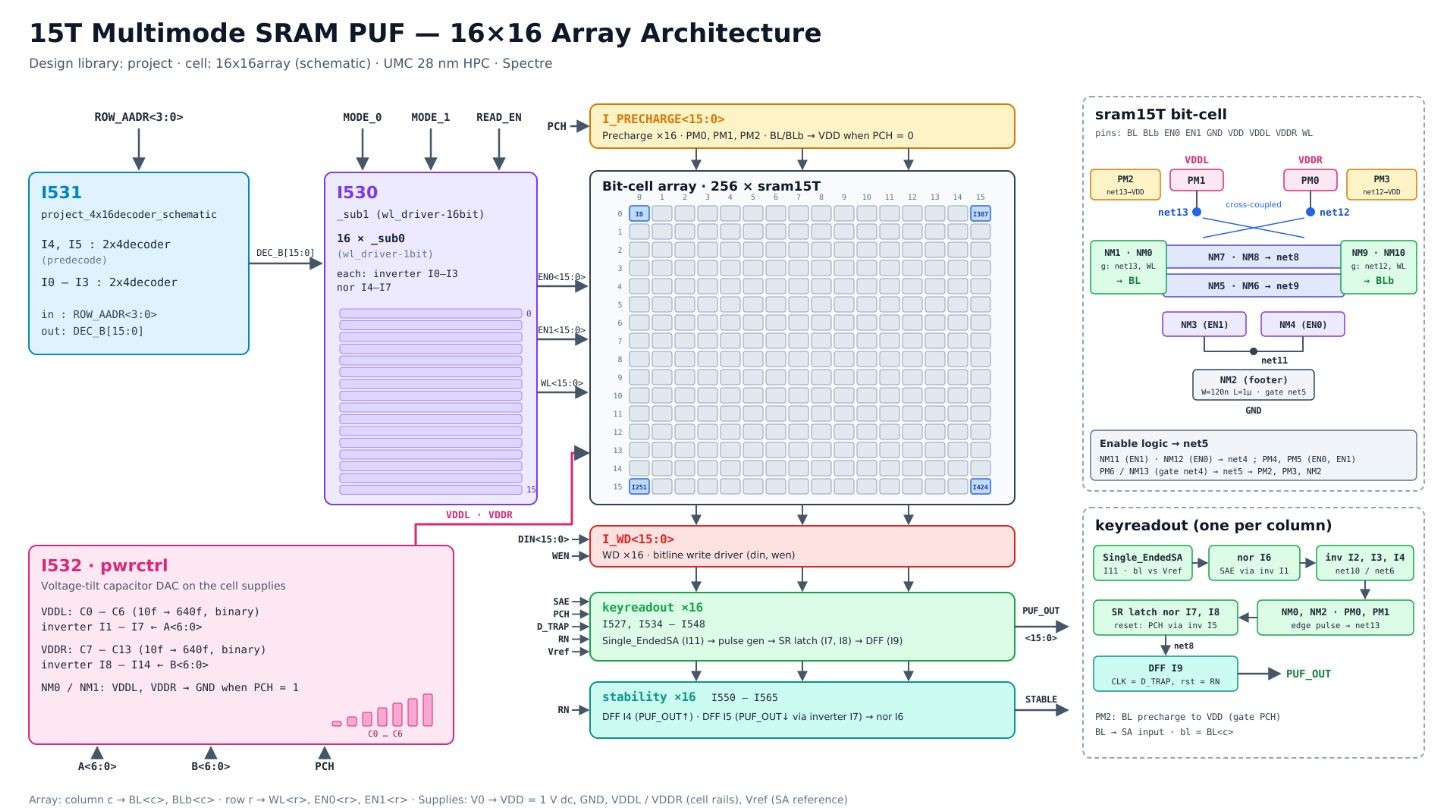
\includegraphics[width=0.94\textwidth]{00_architecture_16x16.jpg}
\caption{Architecture of the implemented 16$\times$16 multimode SRAM PUF (cell \texttt{16x16array}, library \texttt{project}, UMC 28-nm HPC): 4-to-16 decoder (I531), 16-row mode/wordline driver (I530), precharge (I\_PRECHARGE$<$15:0$>$), 256 \texttt{sram15T} cells, write drivers (I\_WD$<$15:0$>$), 16 key-readout circuits, 16 stability-decision circuits and the power-control DAC (I532) generating VDDL/VDDR. Right: bit-cell and key-readout detail.}
\label{fig:arch}
\end{figure*}

\begin{figure*}[!t]
\centering
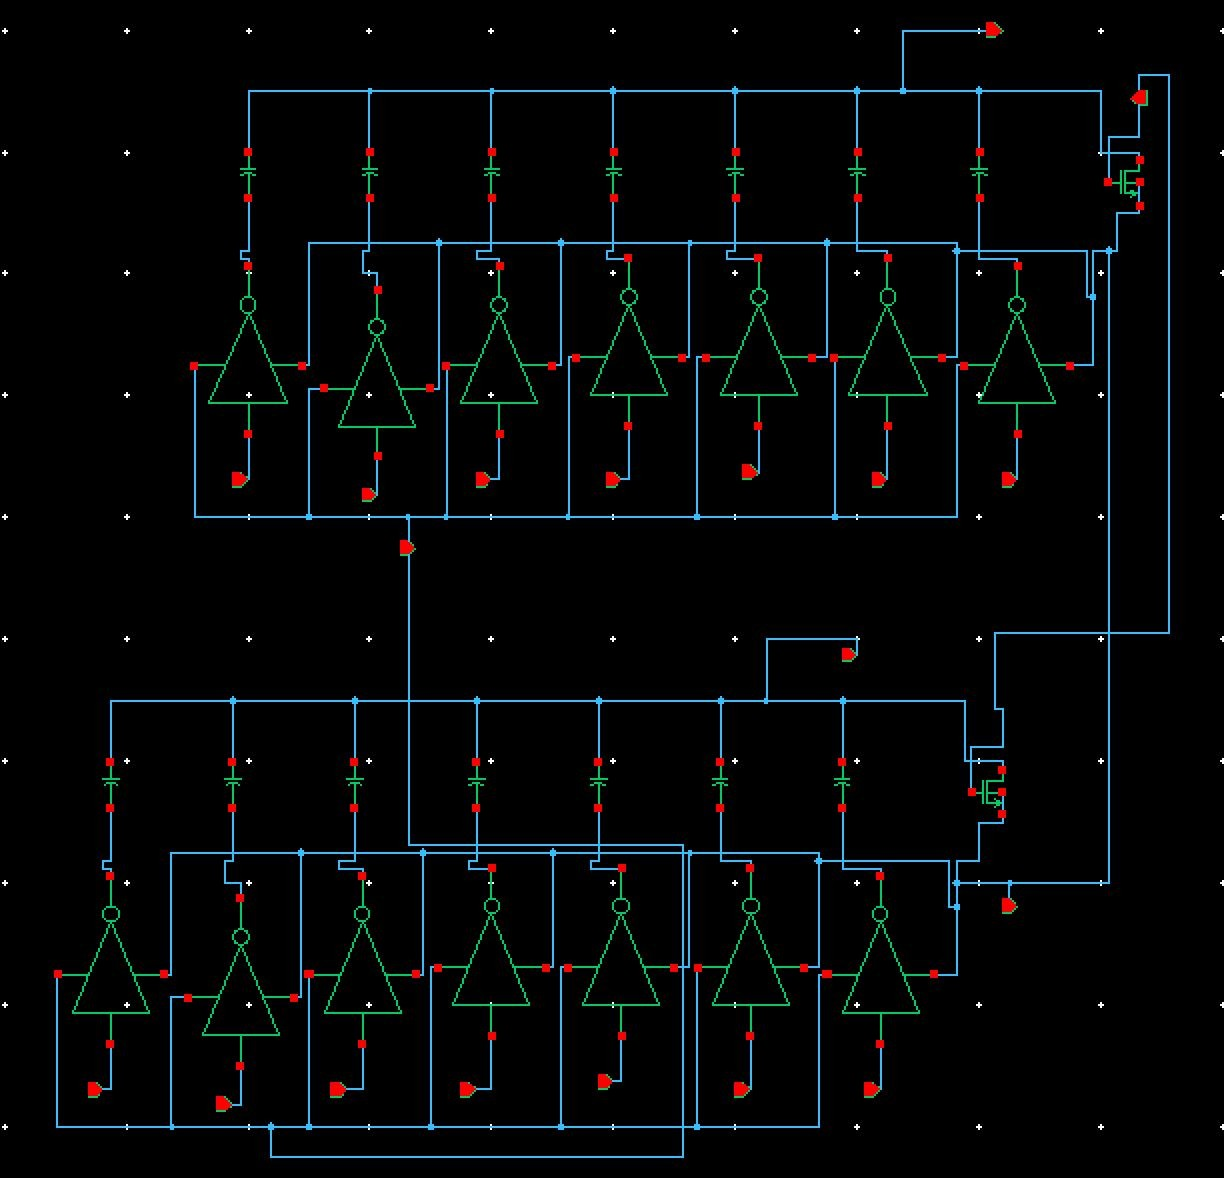
\includegraphics[width=0.56\textwidth]{01_power_control_dac_VDDL_VDDR.jpg}\hfill
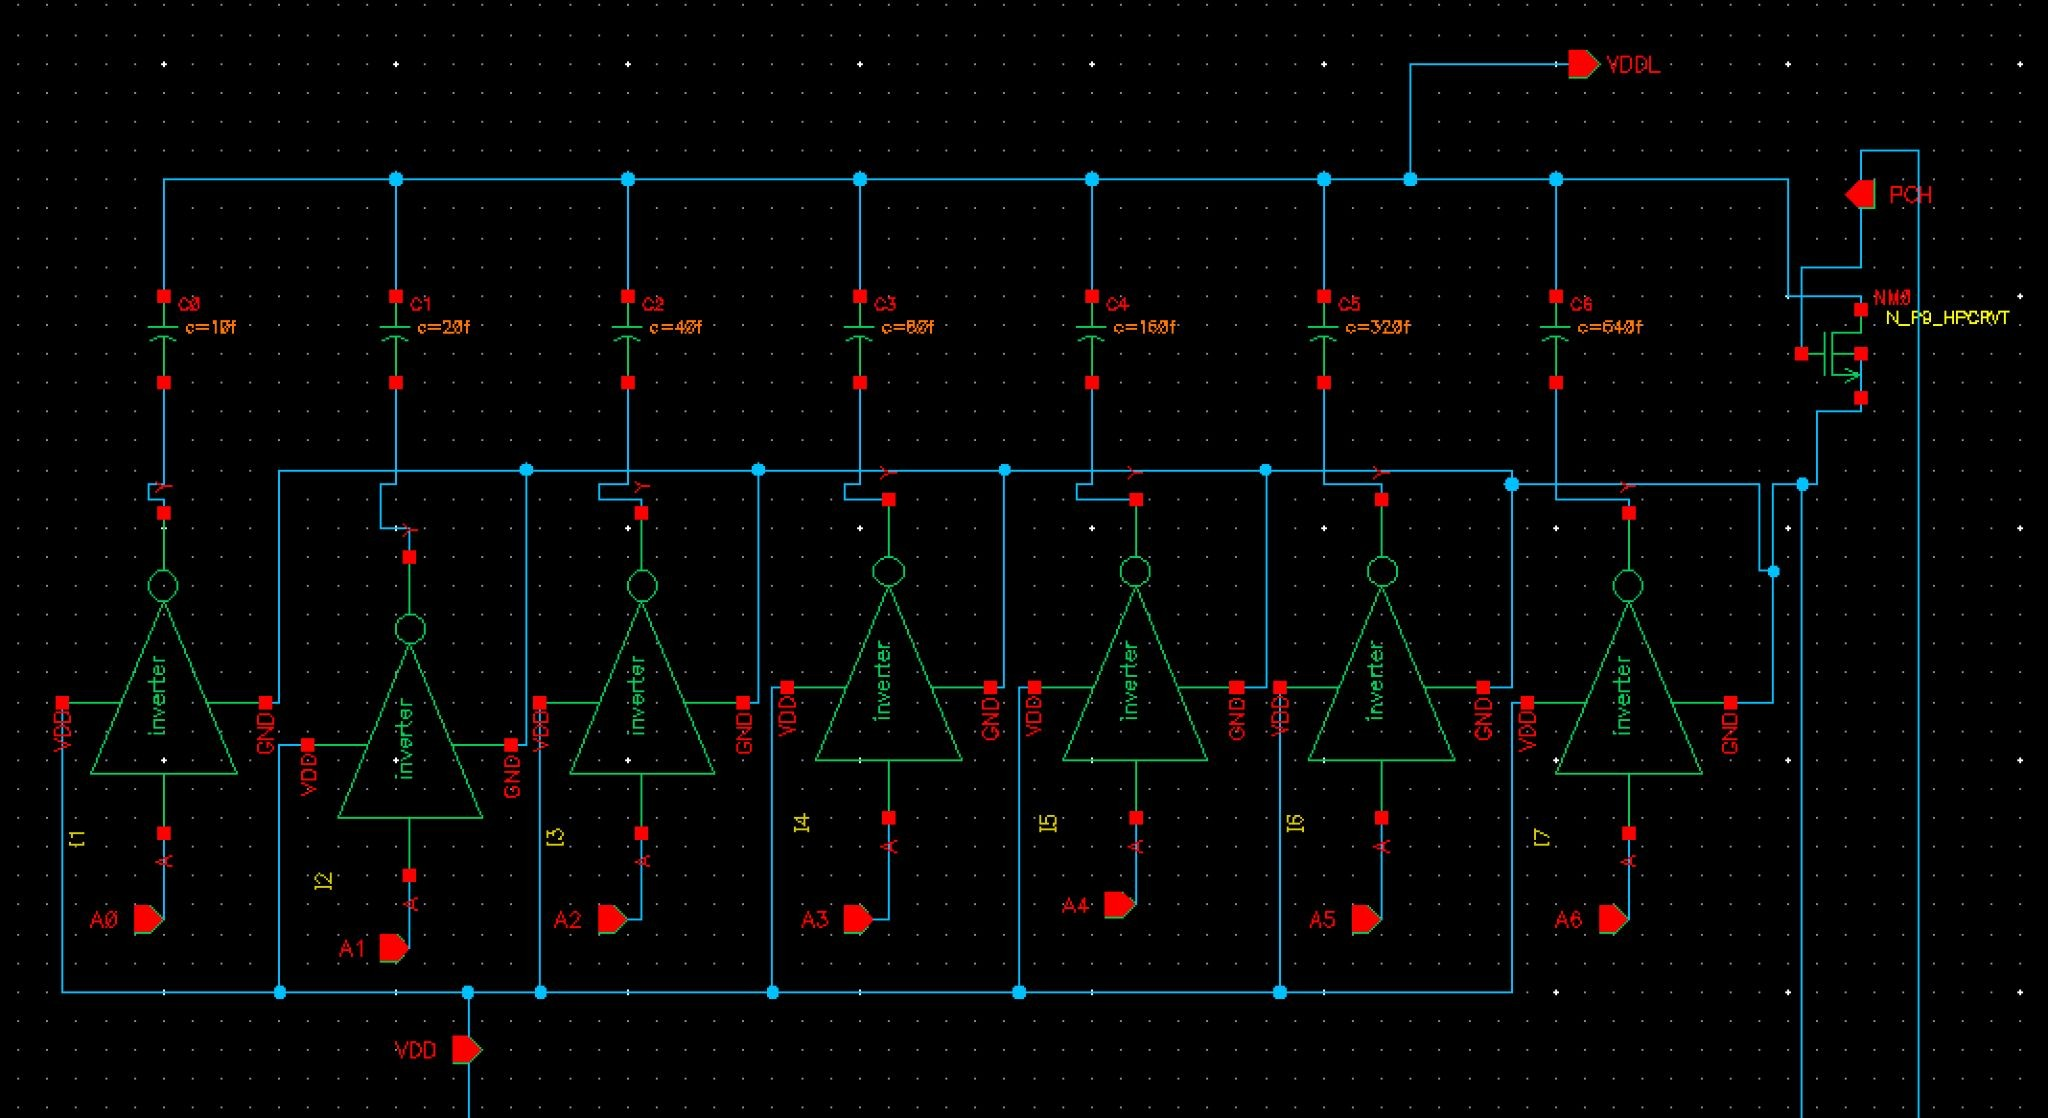
\includegraphics[width=0.42\textwidth]{02_power_control_dac_one_half.jpg}
\caption{Power-control circuit (\texttt{pwrctrl}). Left: complete circuit with two identical 7-bit capacitive DACs; the top half produces VDDL from code A$<$6:0$>$ and the bottom half VDDR from code B$<$6:0$>$. Right: one half, with the binary-weighted capacitors, the inverter switches driving their bottom plates and the PCH-controlled reset transistor.}
\label{fig:dac}
\end{figure*}

\section{Introduction}
\IEEEPARstart{S}{ecure} devices such as satellites need a secret key to prove that they are genuine, but a key stored in non-volatile memory can be read out or copied. A physical unclonable function (PUF) avoids storage altogether: it derives the key each time from the small random differences introduced during manufacturing, which differ from chip to chip and act as a fingerprint \cite{chen2024,phase0}. An SRAM PUF uses a pair of cross-coupled inverters; when both sides start from the same voltage, mismatch between the transistors decides whether the cell settles to 0 or 1, and an array of cells forms the key.

The weakness is reliability. Cells whose two halves are nearly matched settle differently with noise, supply voltage, temperature and radiation, so the key drifts and the bit error rate (BER) rises; two commercial SRAM PUFs exceeded 15\% BER after 100\,krad(Si) \cite{chen2024}. Existing remedies all have a cost \cite{chen2024,phase0}: error-correcting codes add area; temporal majority voting adds power and latency; hot-carrier burn-in accelerates ageing; unstable-bit masking \cite{liu2020} and dark-bit detection \cite{shifman2018} need test time, stored masks and discarded cells; self-checking and healing \cite{he2023} has not been shown under radiation; and a radiation-hardened 8T cell still reaches 2.68\% BER.

Chen \emph{et al.} \cite{chen2024} proposed a 15-transistor multimode SRAM PUF in which each cell produces two independent bits through two separate pull-down pairs. An on-chip voltage-tilt test finds unstable bits, which are then replaced by the cell's second response; only cells unstable in both modes are discarded. Their 55-nm, 4-kb chip reaches 0.0183\% BER after 100\,krad(Si) with self-healing and pre-irradiation masks, 345$\times$ below the raw value.

This project implements that design in UMC 28-nm CMOS \cite{phase2}. Our contributions are:
\begin{enumerate}
\item the 15T cell and a complete 16$\times$16 array in Cadence Virtuoso, with a capacitive power-control DAC, row decoder, mode and wordline drivers, precharge and write drivers, sense-amplifier key readout and stability-decision circuit (Section~III);
\item functional verification of each block, a 2$\times$2 test array and the full array (Section~IV);
\item Monte Carlo characterisation of the 16$\times$16 and 32$\times$64 arrays across supply tilt, supply voltage and temperature (Sections~V--VI); and
\item a comparison of the results within this work and with the silicon results of \cite{chen2024} (Section~VII).
\end{enumerate}

\section{Background: Reference Design}
\subsection{Multimode Cell}
The cell of \cite{chen2024} (Fig.~\ref{fig:paperCell}) has five blocks: a cross-coupled core (M1--M4) whose pMOS pair is shared by both modes; a second nMOS pull-down pair (M11/M12) on the same storage nodes Q/QB; readout transistors (M5, M6, M9, M10) that connect the nodes to BL/BLb through WL without loading them; precharge transistors (M7/M8); and a mode switch (an OR gate and M13--M15). EN1 enables the M3/M4 pair through M13, EN0 the M11/M12 pair through M14, and OR(EN0, EN1) drives the footer M15 and the precharge devices. Table~\ref{tab:modes} lists the modes.

\begin{figure}[!t]
\centering
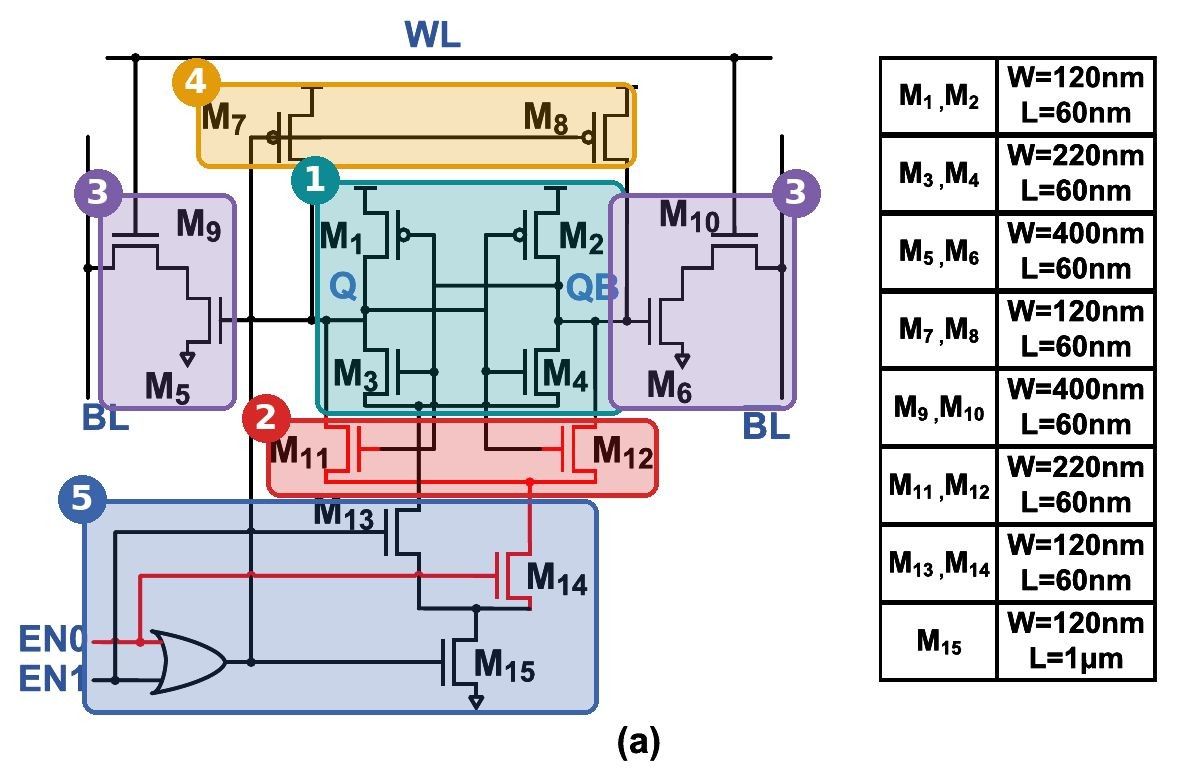
\includegraphics[width=\columnwidth]{paper_15T_cell_annotated_phase0.jpg}
\caption{Reference 15T multimode cell and transistor sizes, from \cite[Fig.~2(a)]{chen2024}, with the block colouring of \cite{phase0}: (1) core, (2) Mode~2 pull-downs, (3) readout, (4) precharge, (5) mode switch.}
\label{fig:paperCell}
\end{figure}

\begin{table}[!t]
\caption{Mode Control \cite{chen2024}}
\label{tab:modes}
\centering
\footnotesize
\begin{tabular}{@{}lccl@{}}
\toprule
Mode & EN0 & EN1 & Discharge path \\
\midrule
Mode 1 & 0 & 1 & Q/QB $\rightarrow$ M3/M4 $\rightarrow$ M13 $\rightarrow$ M15 \\
Mode 2 & 1 & 0 & Q/QB $\rightarrow$ M11/M12 $\rightarrow$ M14 $\rightarrow$ M15 \\
Sleep / precharge & 0 & 0 & none; Q = QB = $\VDD$ \\
\bottomrule
\end{tabular}
\end{table}

One evaluation has four phases \cite{phase2}. In precharge (EN0\,=\,EN1\,=\,0) the precharge transistors hold Q\,=\,QB\,=\,$\VDD$ and there is no path to ground. When one enable rises, the precharge devices turn off and both nodes discharge through the selected pair. In the race that follows, a perfectly matched cell would settle near $\VDD/2$, but mismatch makes one node fall faster. Once $|V_Q-V_{QB}|$ exceeds the separation voltage, positive feedback drives one node to 0 and the other to 1; that is the PUF bit. WL then connects the cell to the bitline for readout, and returning both enables low puts the cell to sleep with no current path.

\subsection{Voltage-Tilt Preselection and Self-Healing}
The two inverters are supplied from separate rails, VDDL and VDDR. Raising one rail and lowering the other by $\Vd$ shifts the inverter trip points apart, so the inverter on the higher supply tends to output 1 \cite{chen2024}. The cell is read with VDDL\,=\,$\VDD+\Vd$, VDDR\,=\,$\VDD-\Vd$ and again with the tilt reversed (Fig.~\ref{fig:paperTilt}). If both reads agree, the cell's mismatch is larger than the tilt and the bit is stable; otherwise it is unstable in that mode and the test is repeated in the other mode.

\begin{figure}[!t]
\centering
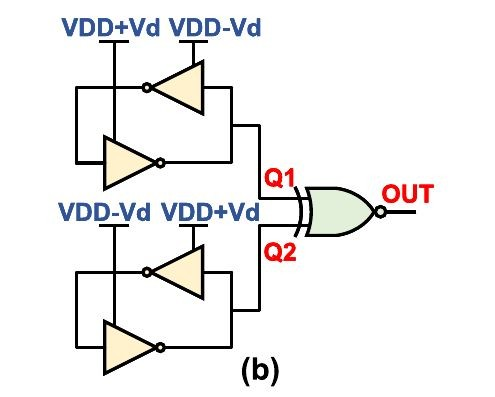
\includegraphics[width=0.62\columnwidth]{paper_voltage_tilt_procedure.jpg}
\caption{Voltage-tilt preselection: the cell is evaluated under both tilt polarities and the two bits Q1, Q2 are compared, from \cite[Fig.~3(b)]{chen2024}.}
\label{fig:paperTilt}
\end{figure}

Fig.~\ref{fig:flow} shows the resulting decision. A cell is \emph{stable} if its Mode~1 bit never flips, \emph{repaired} if Mode~1 flips but Mode~2 does not (the Mode~2 bit is then used), and \emph{discarded} if both modes flip. Valid-bit yield is (stable\,+\,repaired)/$N$ and healing efficiency is repaired/(unstable in Mode~1). Preselection runs once, at enrollment.

\begin{figure}[!t]
\centering
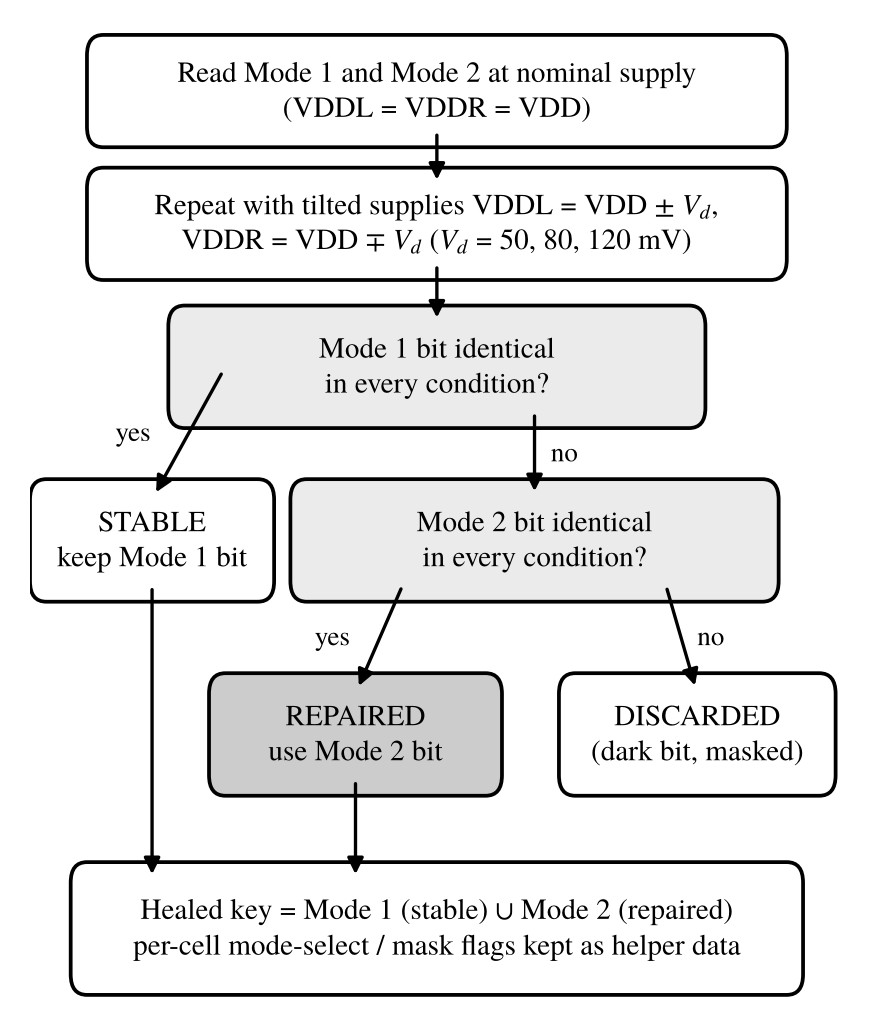
\includegraphics[width=0.80\columnwidth]{selfhealing_flow.jpg}
\caption{Enrollment-time preselection and self-healing decision flow used in this work.}
\label{fig:flow}
\end{figure}

\section{Circuit Implementation in UMC 28\,nm}
\subsection{Array Architecture}
Fig.~\ref{fig:arch} shows the implemented architecture. A 4-bit row address ROW\_ADDR$<$3:0$>$ is decoded into sixteen active-low row selects DEC\_B$<$15:0$>$. The mode and wordline driver combines these with MODE\_0, MODE\_1 and READ\_EN to produce EN0, EN1 and WL for each row. Each of the sixteen columns has a precharge circuit, a write driver, a key-readout circuit and a stability-decision circuit, and the power-control DAC supplies the tilted rails VDDL and VDDR to the cells. Column $c$ connects to BL$<c>$/BLb$<c>$ and row $r$ to WL$<r>$, EN0$<r>$ and EN1$<r>$. Rows are evaluated and read one at a time, so only sixteen cells draw current at once and unselected cells do not load the bitlines.

\subsection{15T Bit-Cell}
Fig.~\ref{fig:cell} is the Cadence schematic of the cell (\texttt{sram15T}; pins BL, BLb, EN0, EN1, GND, VDD, VDDL, VDDR, WL). The cross-coupled pMOS pair PM0/PM1 is supplied from VDDR and VDDL; the two nMOS pull-down pairs NM7/NM8 and NM5/NM6 give the two modes and are selected by NM3 (EN1) and NM4 (EN0). NM2 is the footer (W/L\,=\,120\,nm/1\,$\mu$m, as in \cite{chen2024}), kept weak so that the race is decided by the core rather than by the footer \cite{phase0}. PM2/PM3 precharge the storage nodes, NM0/NM1 and NM9/NM10 form the WL-gated readout to BL and BLb, and the OR of EN0 and EN1 is built from NM11, NM12, PM4, PM5 (NOR) followed by PM6/NM13 (inverter) driving net5, which controls the precharge devices and the footer.

\begin{figure}[!t]
\centering
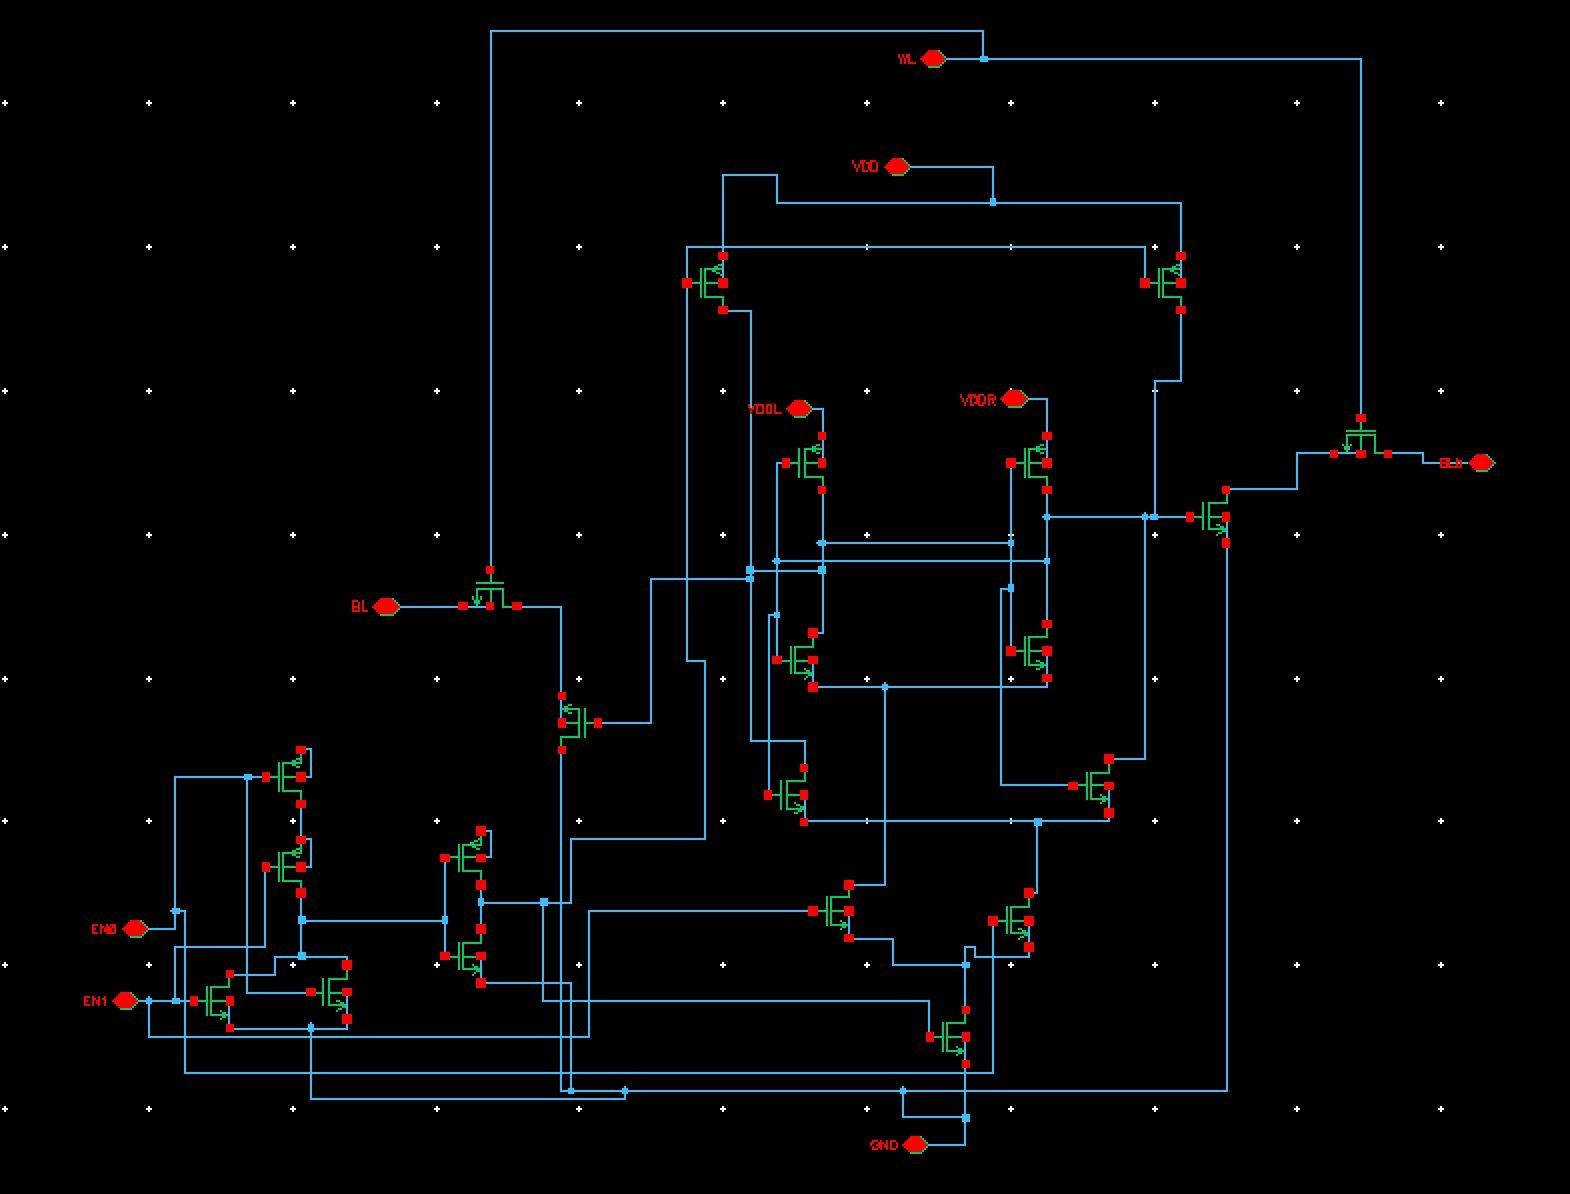
\includegraphics[width=\columnwidth]{01_sram15T_bitcell.jpg}
\caption{Cadence schematic of the 15T multimode bit-cell with the EN0/EN1 OR gate.}
\label{fig:cell}
\end{figure}

\subsection{Power-Control DAC}
The power-control circuit (Fig.~\ref{fig:dac}) generates VDDL and VDDR for the tilt test. It has two identical halves; each is a 7-bit charge-redistribution DAC with binary-weighted capacitors (10\,fF to 640\,fF) whose top plates form the output node. Each bottom plate is driven by a CMOS inverter acting as a two-way switch: input 0 ties the plate to VDD, input 1 to VSS. In operation \cite{phase2}: (1) PCH turns on an nMOS that discharges the output to 0\,V; (2) the 7-bit code connects selected bottom plates to VDD and the rest to VSS; (3) charge redistributes and the output settles at $V_{\mathrm{out}}=\VDD\times\mathrm{code}/127$, a step of about 7--8\,mV. The VDD/VSS buses and PCH are shared, while each half has its own code (A$<$6:0$>$ for VDDL, B$<$6:0$>$ for VDDR), so the two rails can be set independently. A capacitive DAC draws almost no static power, is programmable and is compact.

\subsection{Row Control: Decoder, Wordline and Mode Drivers}
The 4-to-16 decoder (Fig.~\ref{fig:dec}) is built from two 2-to-4 decoders used as predecoders and four 2-to-4 decoders for the final selection, producing DEC\_B$<$15:0$>$. The one-bit wordline driver (Fig.~\ref{fig:wl}, left) generates WL, EN0 and EN1 for one row; each output is a NOR gate with active-low inputs, with inverters on the active-high inputs. Only the selected row receives WL and an enable; unselected rows keep WL\,=\,EN0\,=\,EN1\,=\,0 and stay in sleep. The sixteen-bit driver (Fig.~\ref{fig:wl}, right) instantiates sixteen of these. The complete row-control block (Fig.~\ref{fig:modewl}) works as follows: ROW\_ADDR\,=\,$k$ sets DEC\_B$<k>$\,=\,0; MODE\_0 or MODE\_1 then raises only EN0$<k>$ or EN1$<k>$ so that row $k$ evaluates in the chosen mode; READ\_EN raises WL$<k>$ and the row's sixteen bits go to the sixteen readout circuits. Repeating for $k=0$ to 15 scans all 256 bits.

\begin{figure}[!t]
\centering
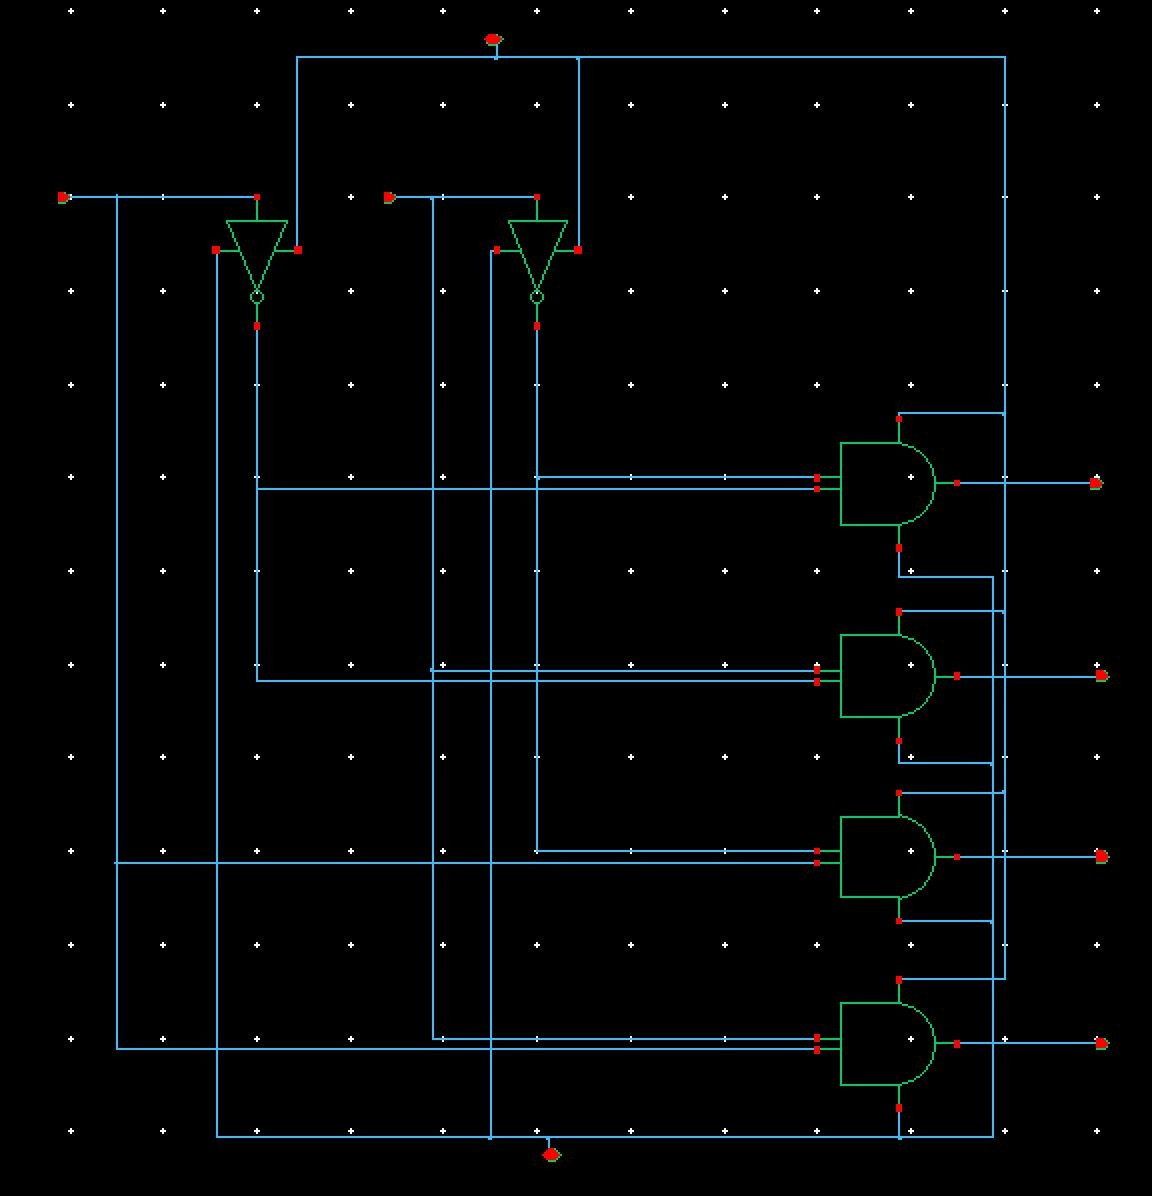
\includegraphics[width=0.49\columnwidth]{08_decoder_2x4.jpg}\hfill
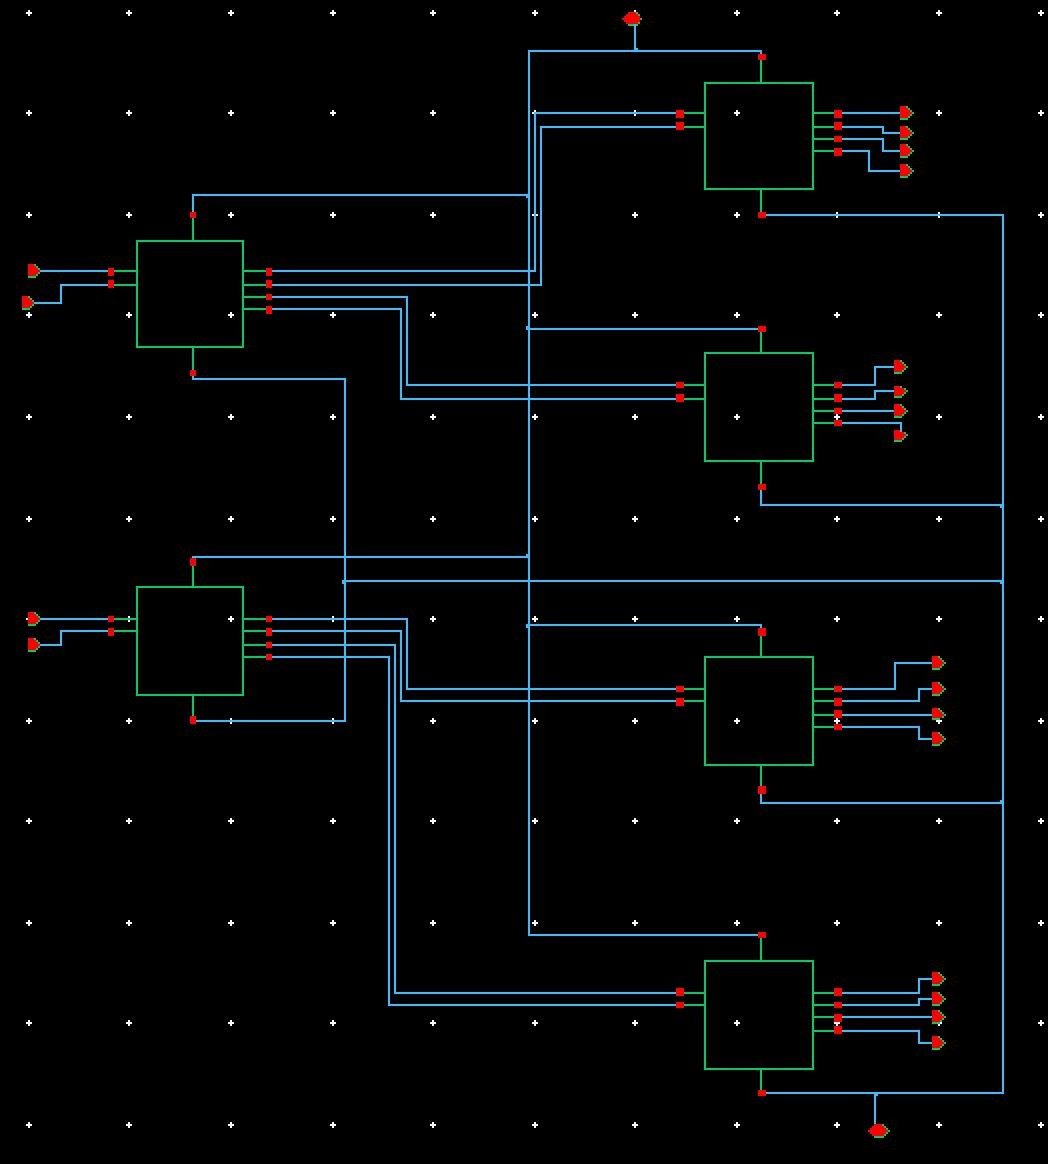
\includegraphics[width=0.49\columnwidth]{09_decoder_4x16.jpg}
\caption{Row decoder: 2-to-4 decoder (left) and the 4-to-16 decoder built from it (right).}
\label{fig:dec}
\end{figure}

\begin{figure}[!t]
\centering
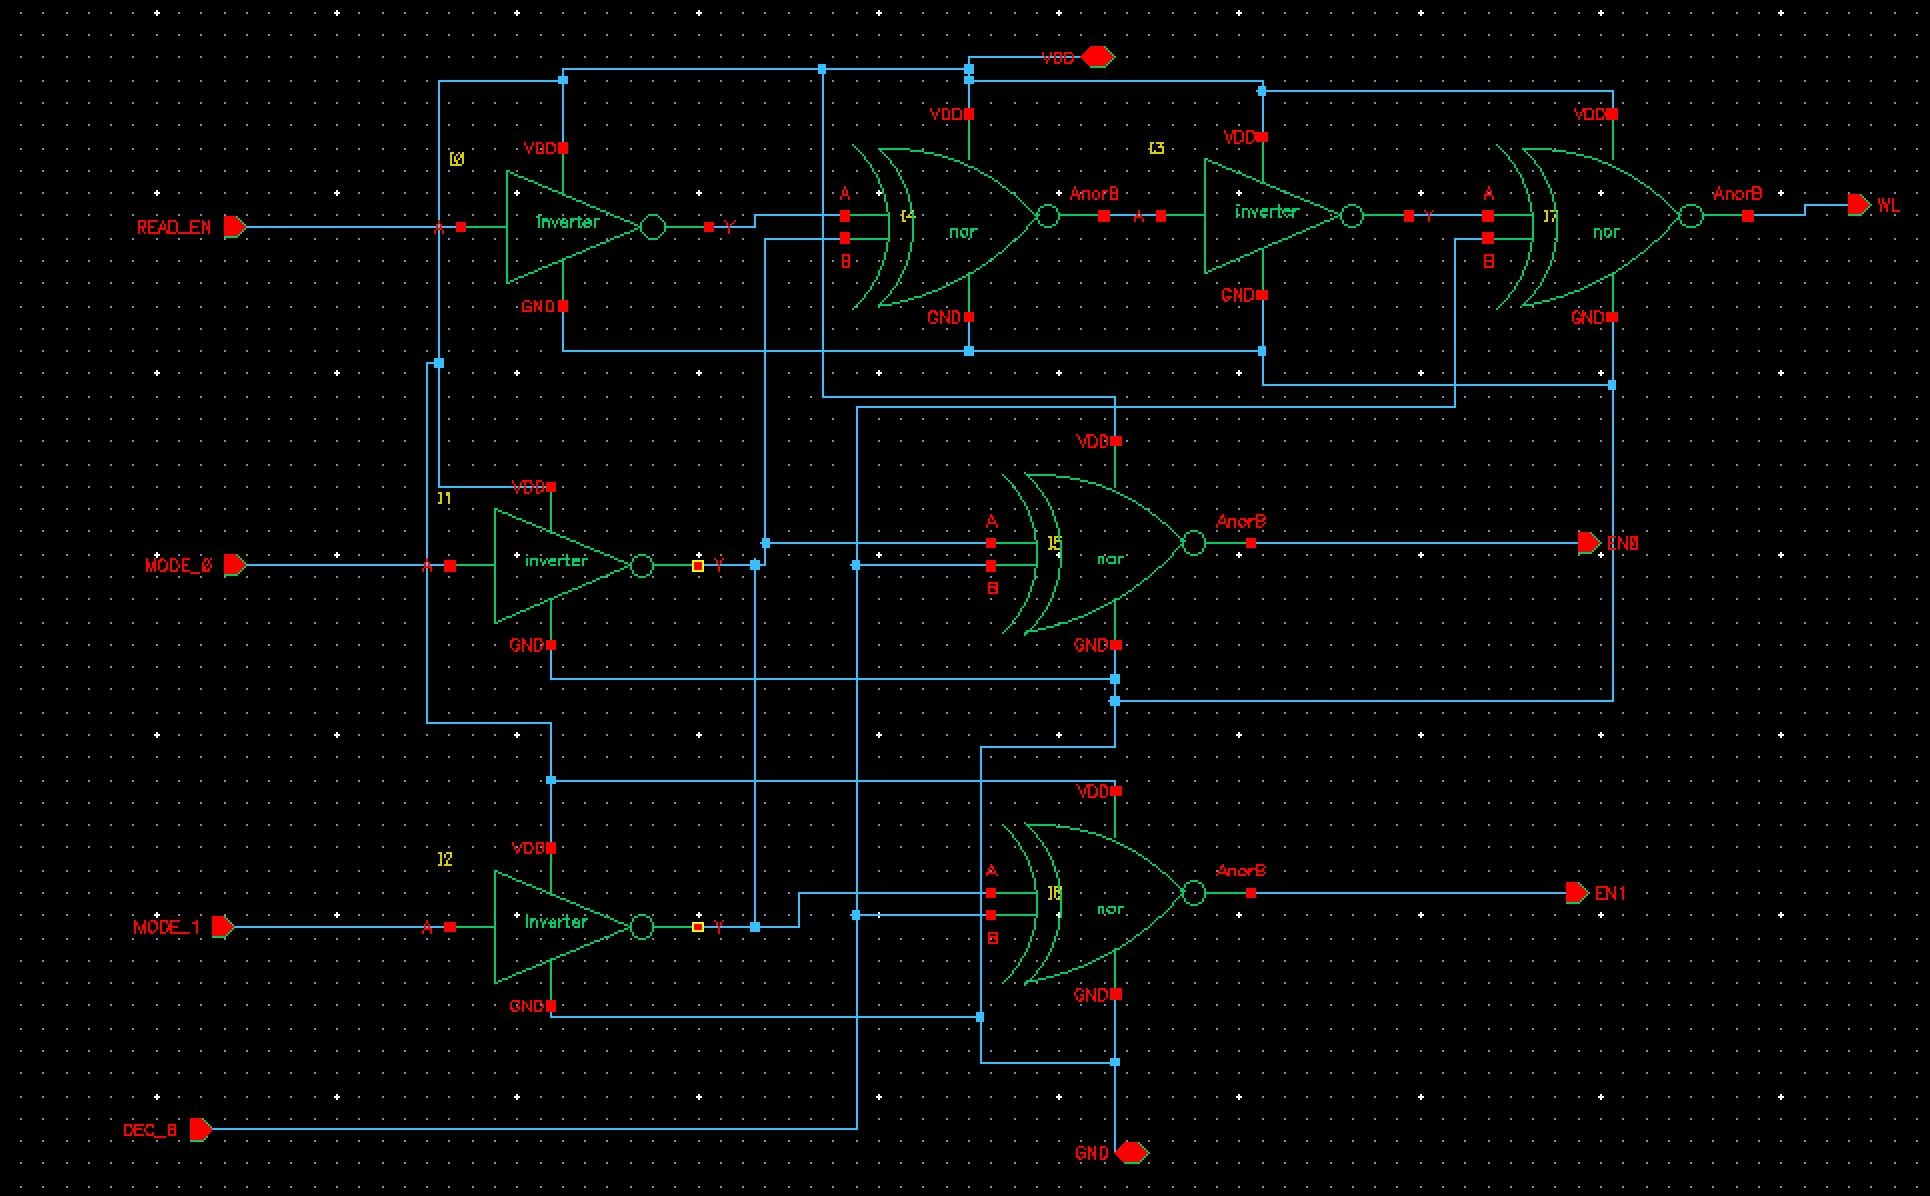
\includegraphics[width=0.56\columnwidth]{06_wl_driver_1bit.jpg}\hfill
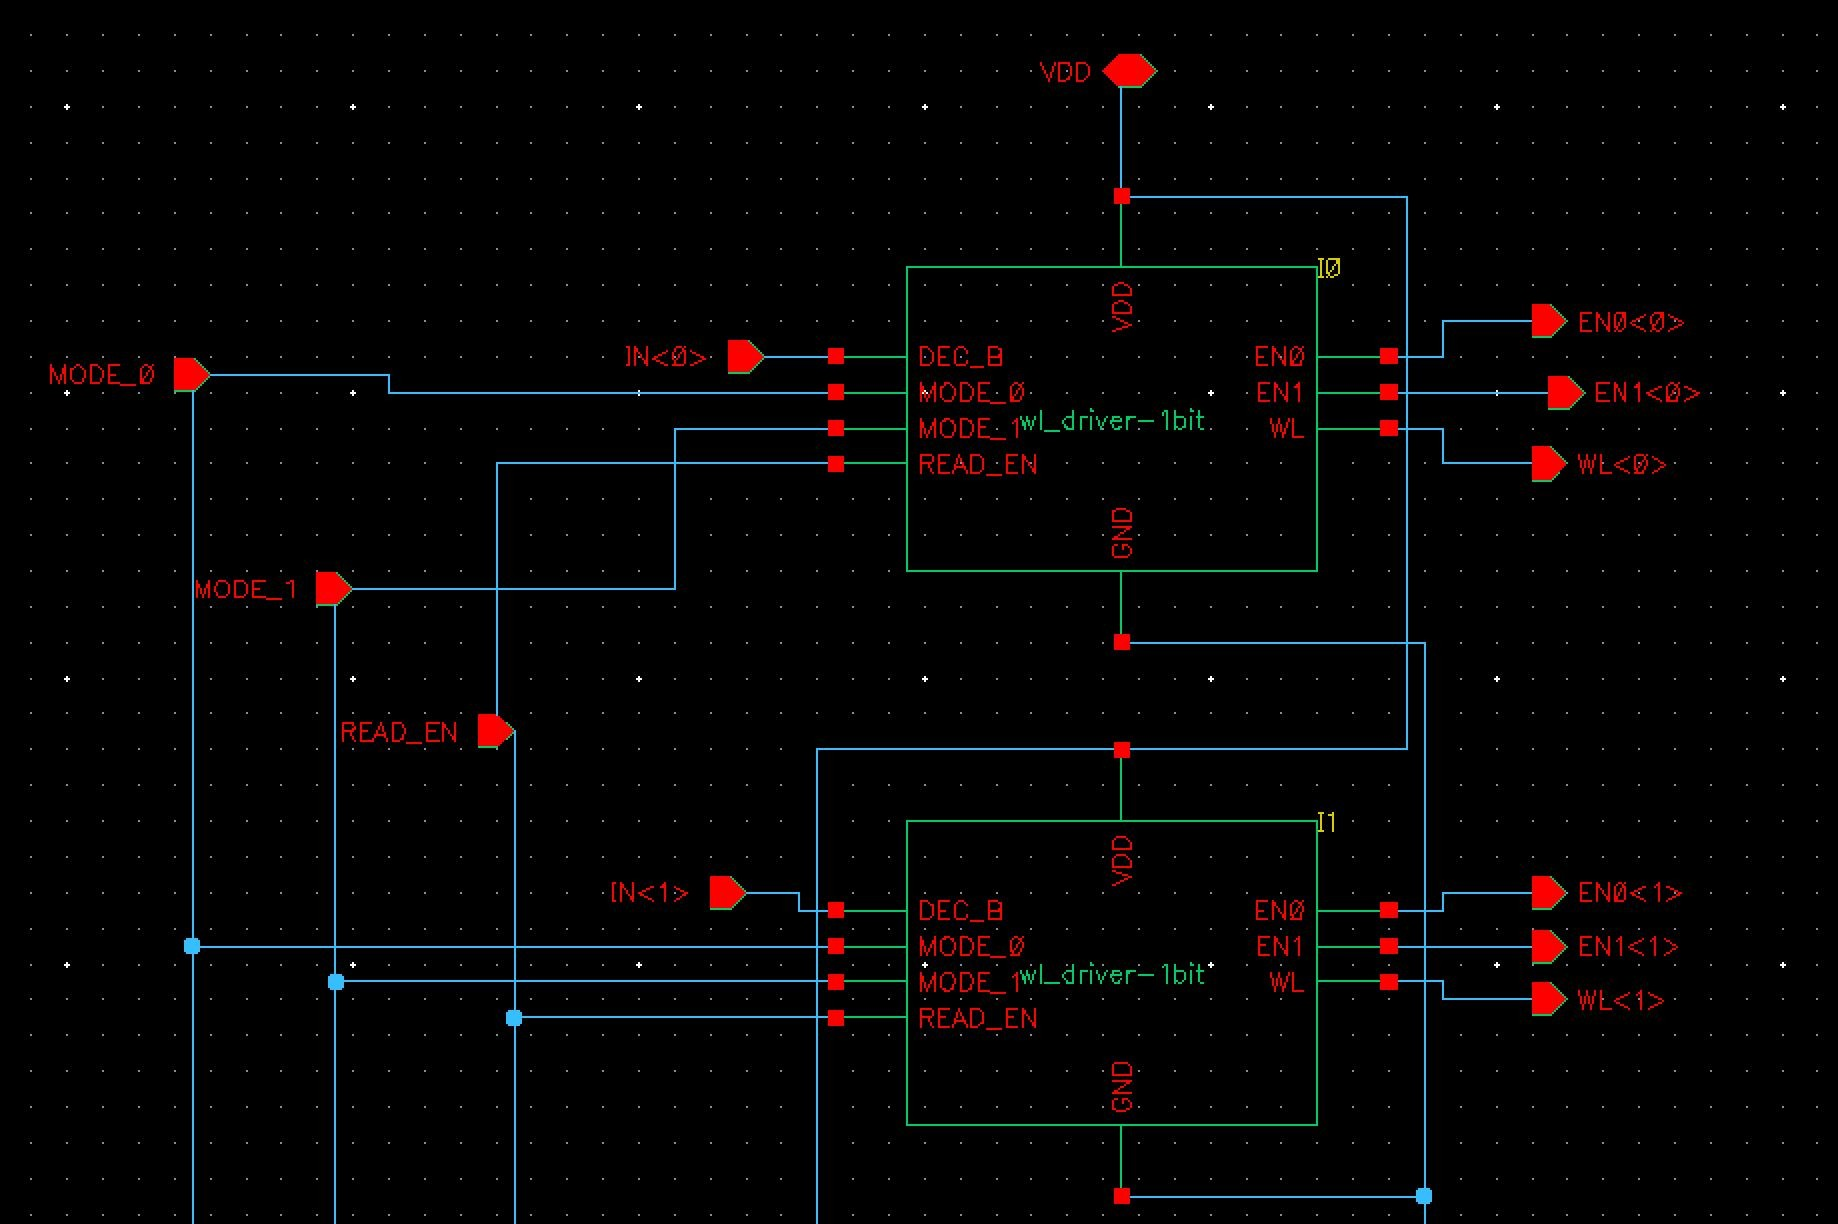
\includegraphics[width=0.42\columnwidth]{07_wl_driver_16bit.jpg}
\caption{Wordline/mode driver for one row (left) and the sixteen-row driver (right).}
\label{fig:wl}
\end{figure}

\begin{figure}[!t]
\centering
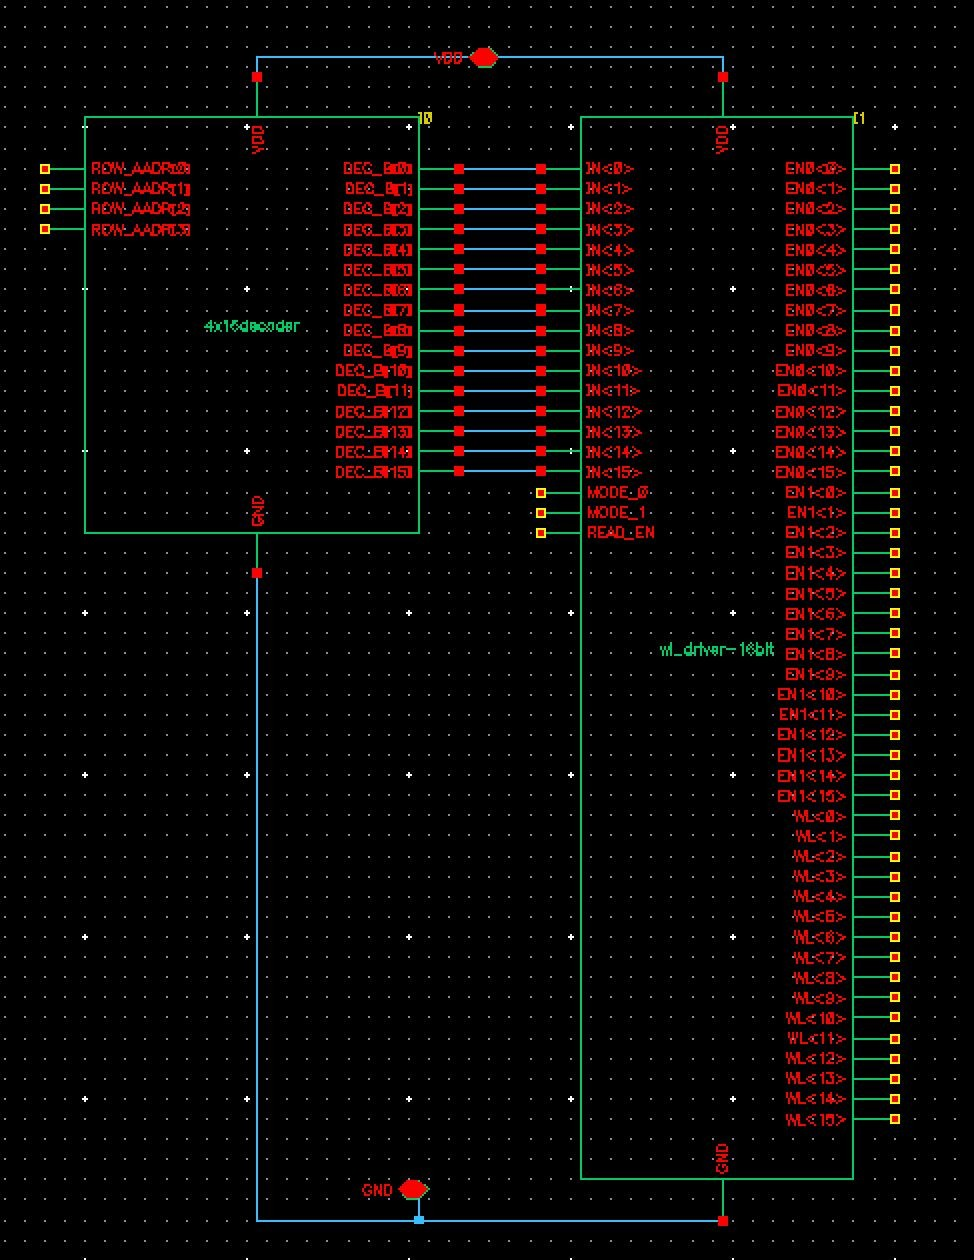
\includegraphics[width=0.62\columnwidth]{13_mode_wl_driver.jpg}
\caption{Row-control block (\texttt{mode\_wl\_driver}): 4-bit row address to WL, EN0 and EN1 for all sixteen rows.}
\label{fig:modewl}
\end{figure}

\subsection{Bitline Precharge and Write Driver}
The precharge circuit (Fig.~\ref{fig:pchwd}, left) pulls BL and BLb to VDD when PCH is low. The write driver (Fig.~\ref{fig:pchwd}, right) forces BL\,=\,din and BLb\,=\,$\overline{\mathrm{din}}$ strongly enough to overwrite a cell when write is enabled, and disconnects (high impedance) when write is disabled, leaving the bitlines free for reading. The write driver, sense amplifier and flip-flop are adapted from cells provided by the course teaching assistants \cite{phase2}.

\begin{figure}[!t]
\centering
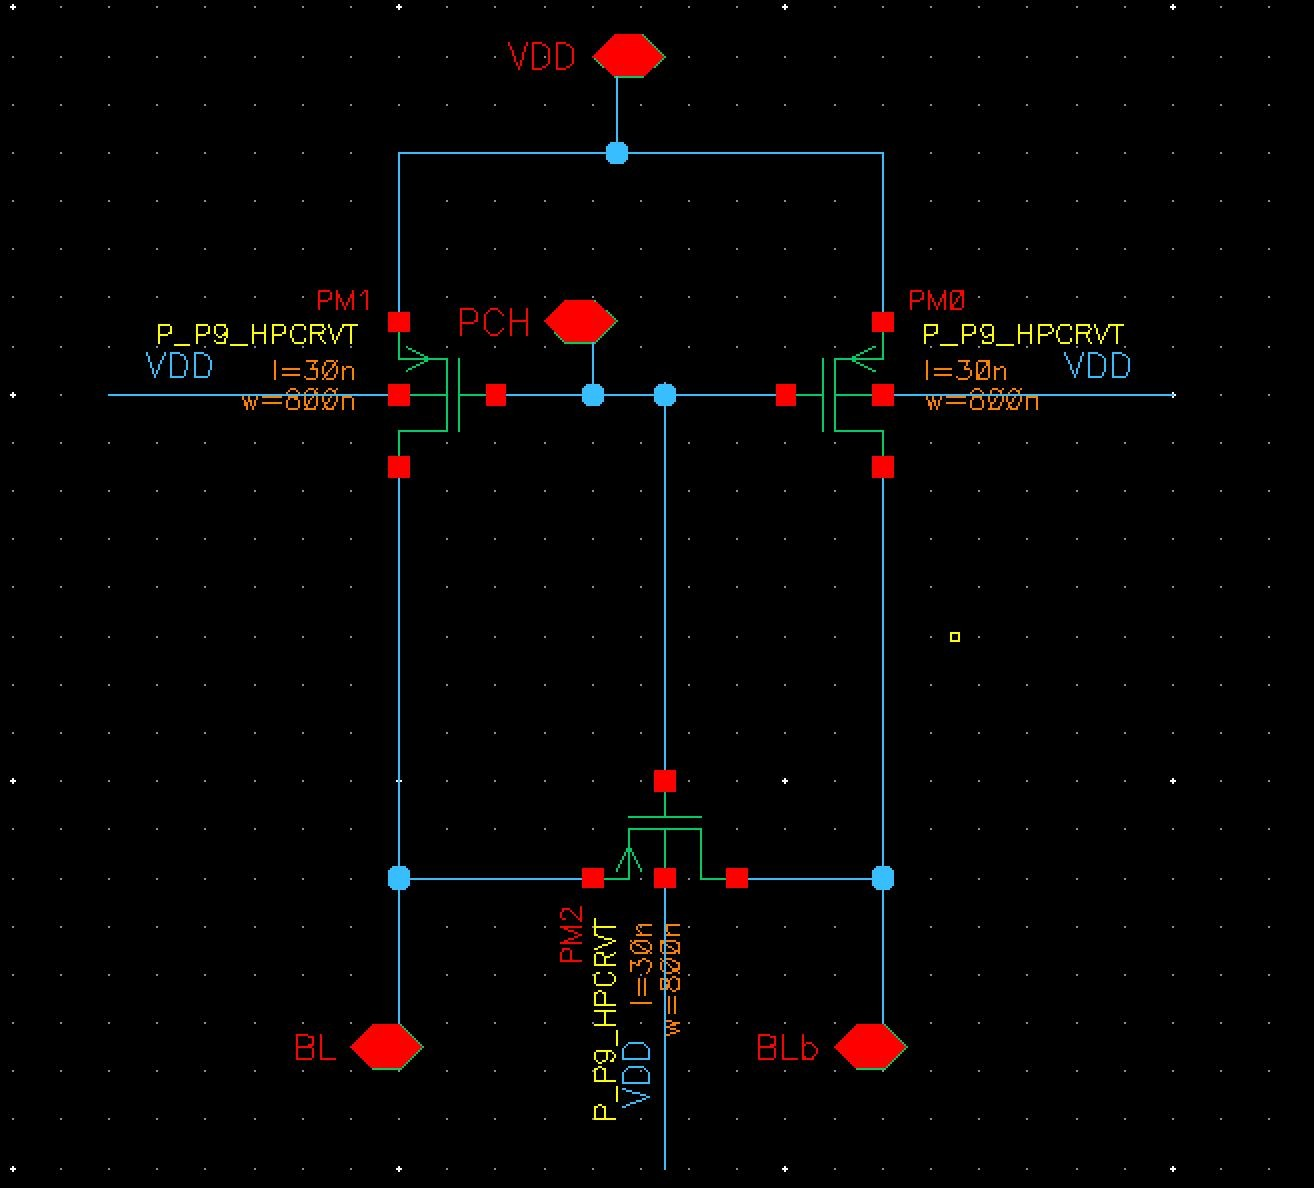
\includegraphics[width=0.40\columnwidth]{10_precharge.jpg}\hfill
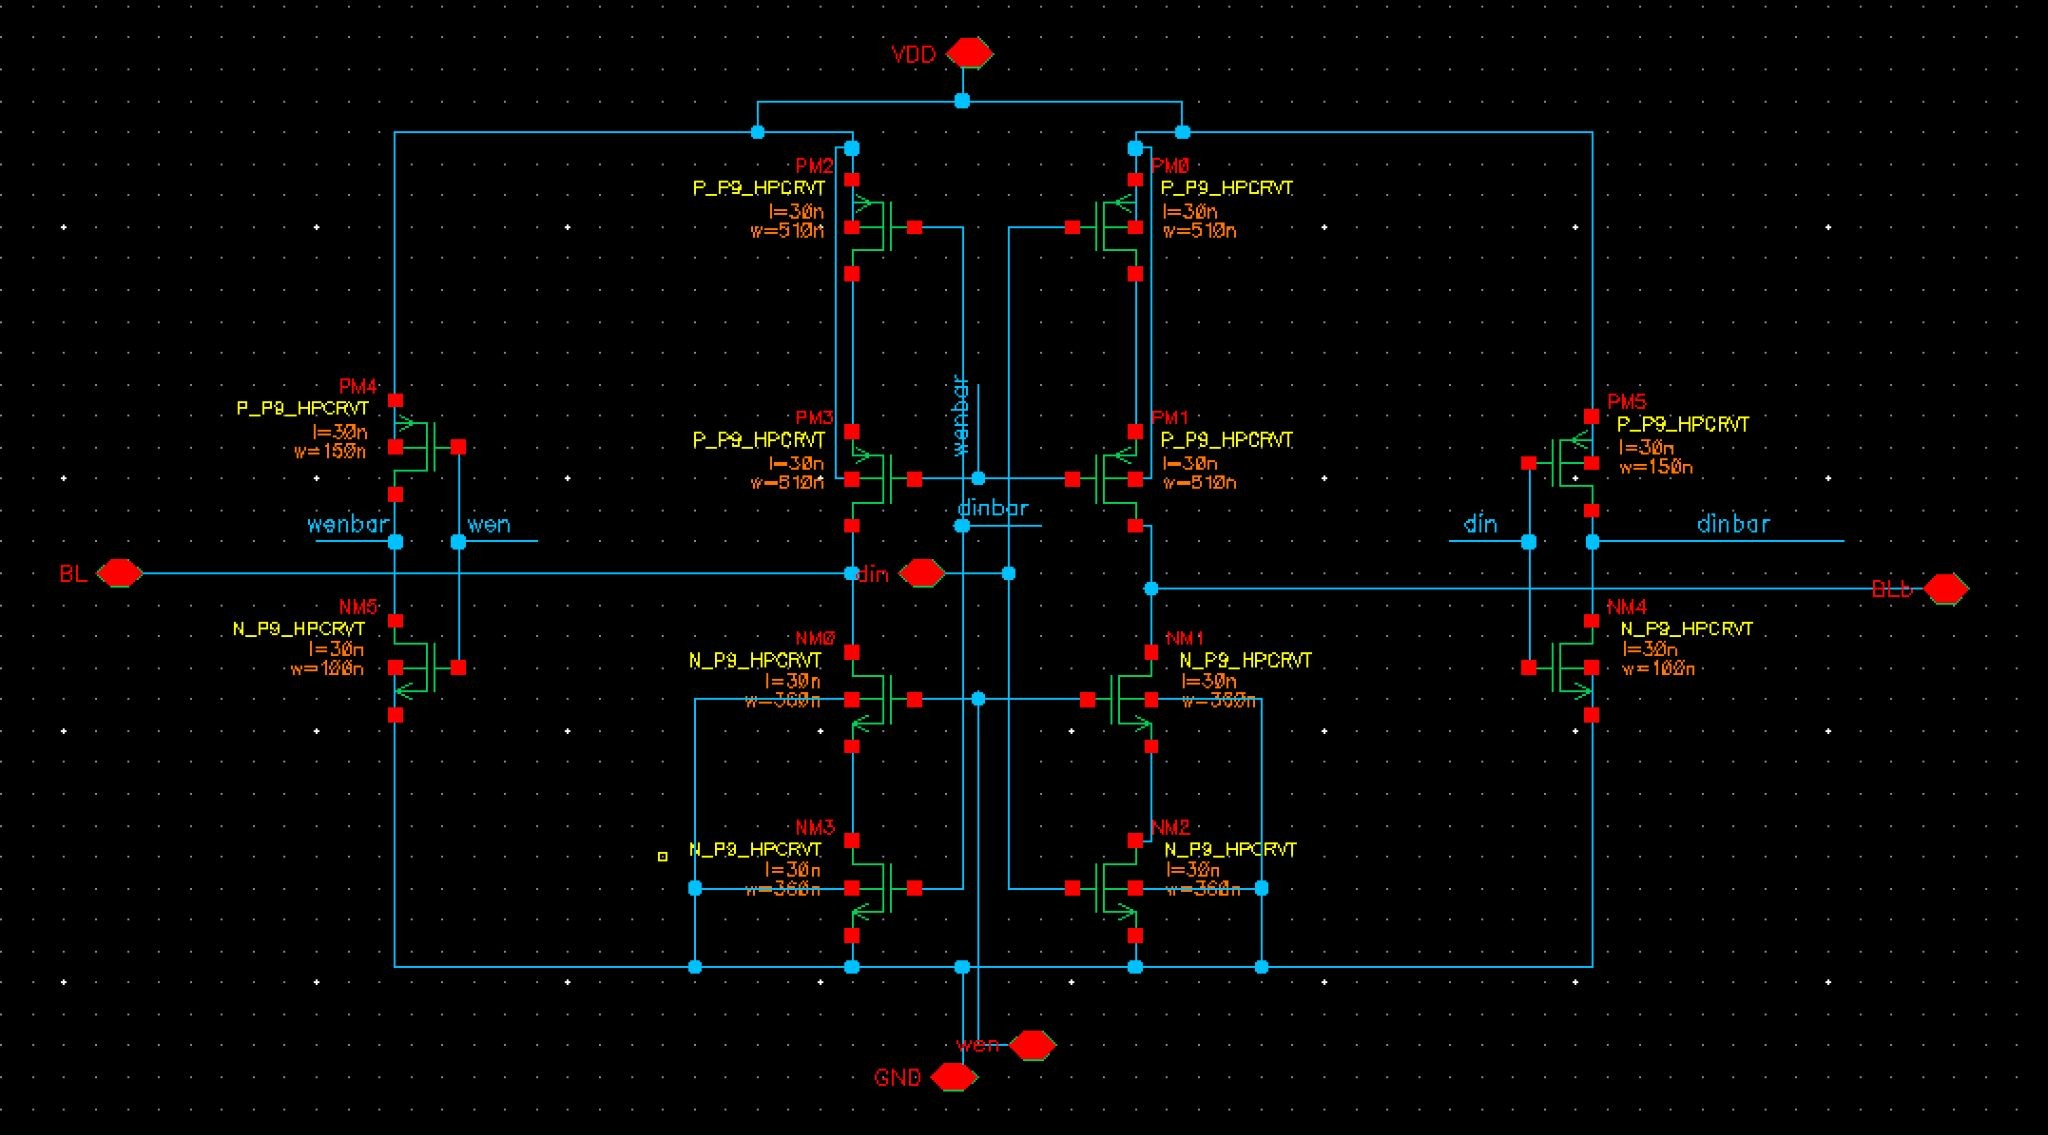
\includegraphics[width=0.58\columnwidth]{12_write_driver.jpg}
\caption{Bitline precharge (left) and write driver (right).}
\label{fig:pchwd}
\end{figure}

\subsection{Key Readout and Sense Amplifier}
The key-readout circuit (Fig.~\ref{fig:readout}) turns the slow analog bitline into a clean, glitch-free PUF OUT \cite{phase2}. During precharge (PCH\,=\,0) BL is charged to VDD and the sense amplifier is off. When WL rises the cell is connected to BL: a stored 0 discharges BL slowly while a stored 1 leaves it high. After BL has settled, SAE fires and the single-ended sense amplifier (Fig.~\ref{fig:sa}) compares BL with VREF, using positive feedback to produce a full-swing output. The direct output and a delayed copy (through a two-inverter buffer and one more inverter) drive a four-transistor stack, so the output flips only if a new value persists longer than the delay; this rejects race-condition glitches. An SR latch (NOR pair, reset by PCH) holds the value, and the D\_TRAP edge clocks it into a D flip-flop whose output is PUF OUT.

\begin{figure}[!t]
\centering
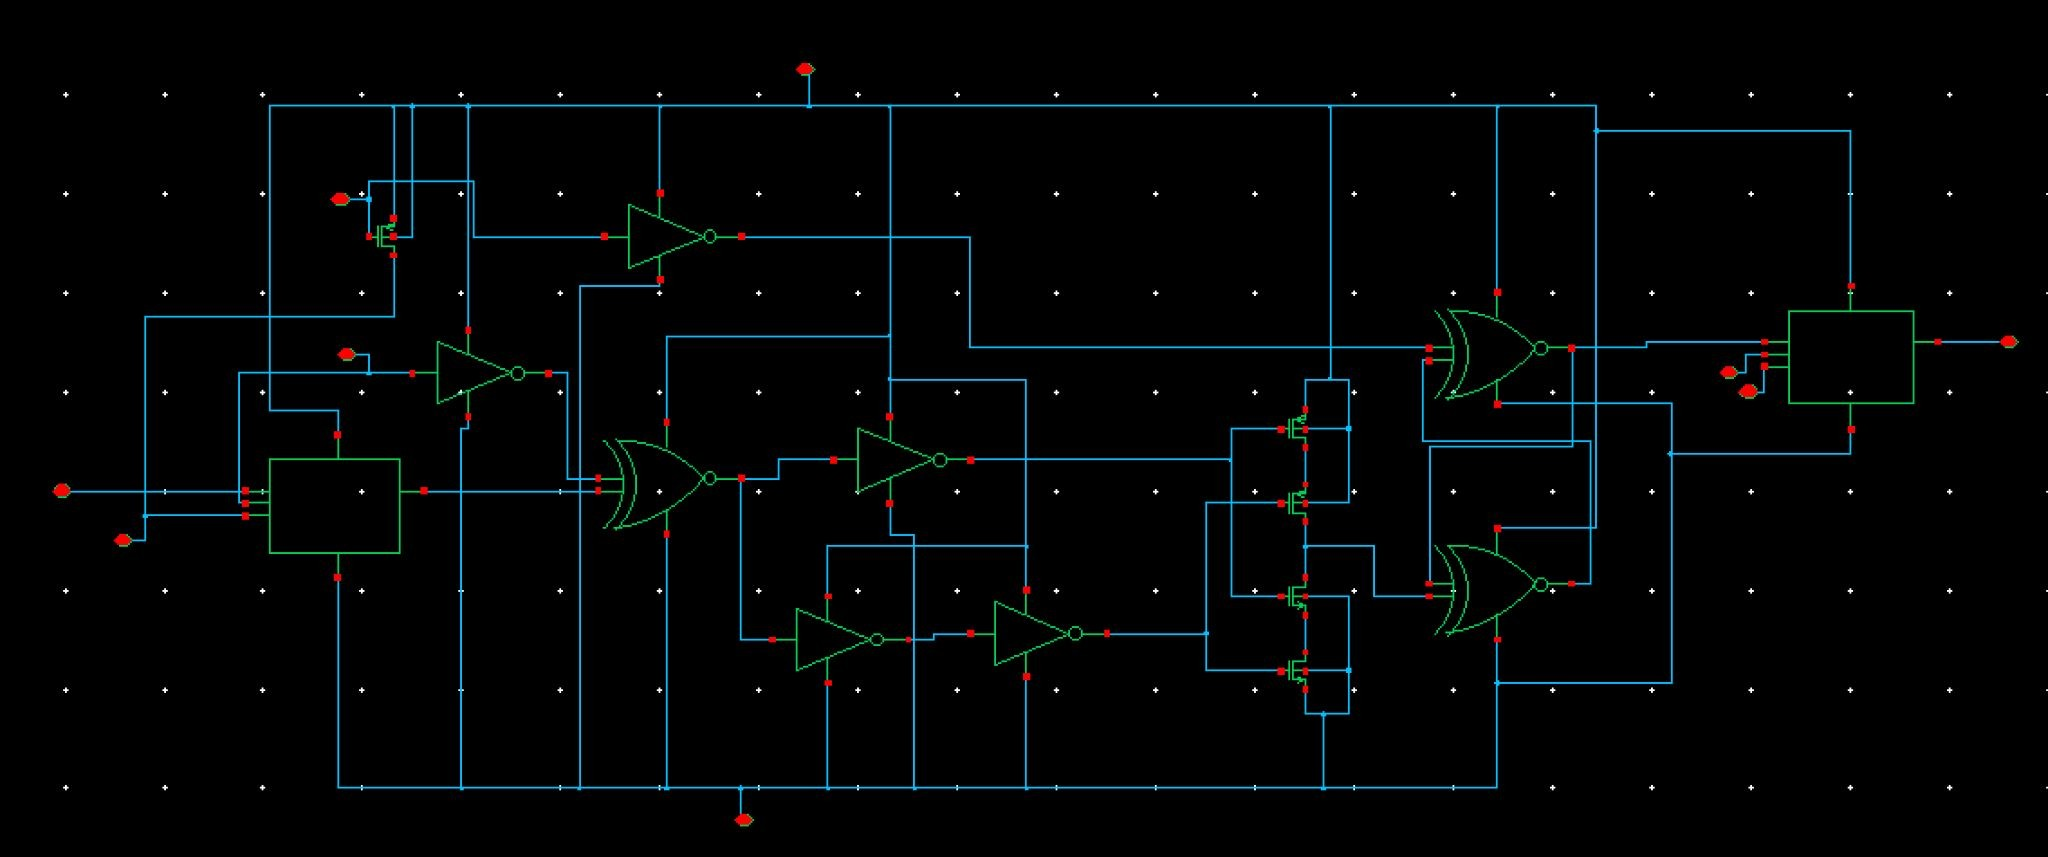
\includegraphics[width=\columnwidth]{03_key_readout.jpg}
\caption{Key-readout circuit: single-ended sense amplifier, glitch filter, SR latch and output flip-flop.}
\label{fig:readout}
\end{figure}

\begin{figure}[!t]
\centering
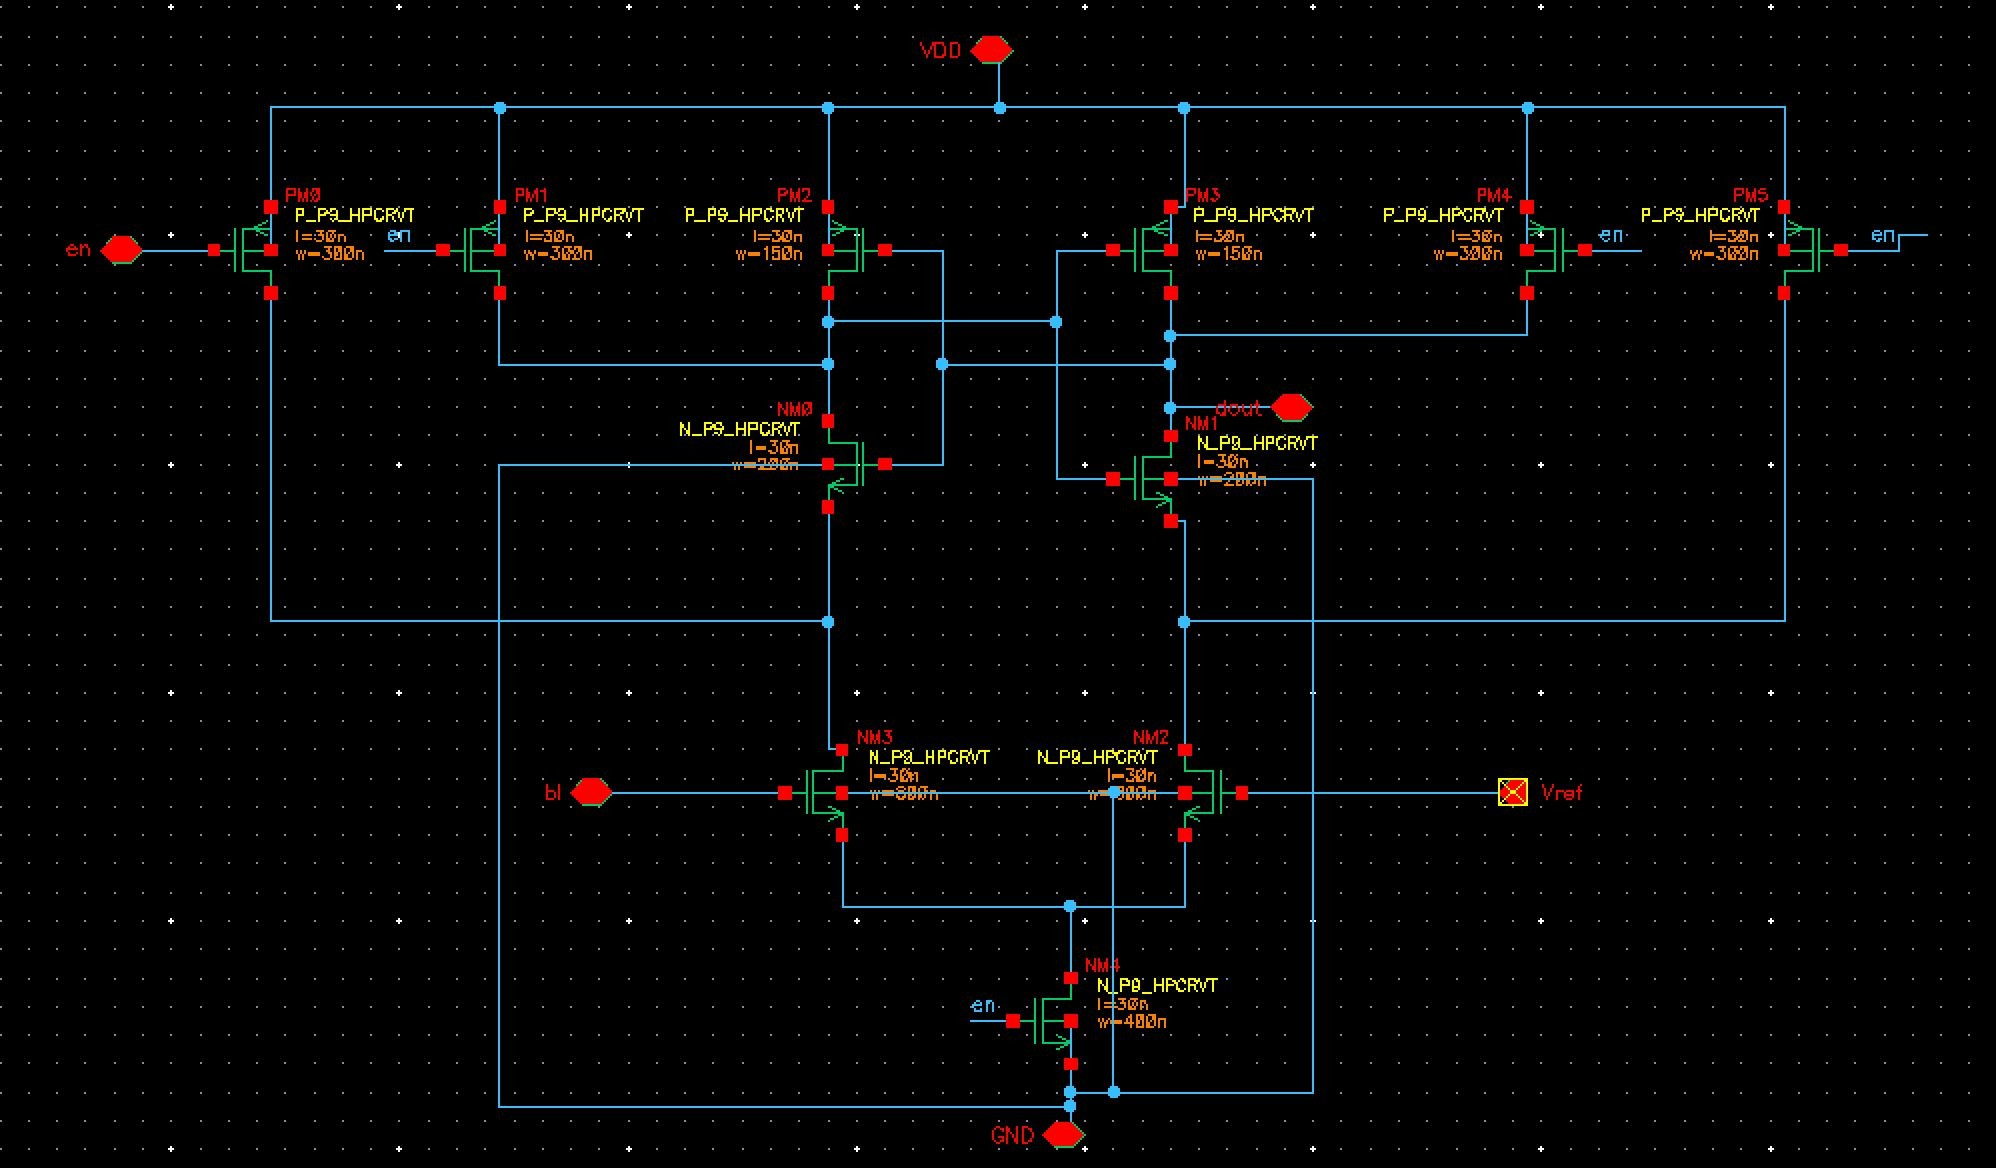
\includegraphics[width=0.92\columnwidth]{11_single_ended_sense_amplifier.jpg}
\caption{Single-ended sense amplifier comparing BL with VREF.}
\label{fig:sa}
\end{figure}

\subsection{Stability Decision}
The stability-decision circuit (Fig.~\ref{fig:stab}) checks whether a cell gave the same bit in both tilt tests \cite{phase2}. Pulsing RN resets both D flip-flops (D tied to 1), so the NOR output STABLE is 1. In stage 1 (tilt A, VDDL high) the readout places the bit on PUF\_OUT; in stage 2 (tilt B, VDDR high) the cell is re-evaluated and PUF\_OUT updates. If the bit is unchanged there is no edge and STABLE stays 1. A 0$\rightarrow$1 change clocks DFF1 directly; a 1$\rightarrow$0 change becomes a rising edge after an inverter and clocks DFF2; either way STABLE falls to 0 and the cell is healed or masked. A flip-flop with D\,=\,1 acts as an edge detector with memory, so even a short flip stays flagged until the next reset. The flip-flop (Fig.~\ref{fig:dff}) was given a reset pin for the active-low RN.

\begin{figure}[!t]
\centering
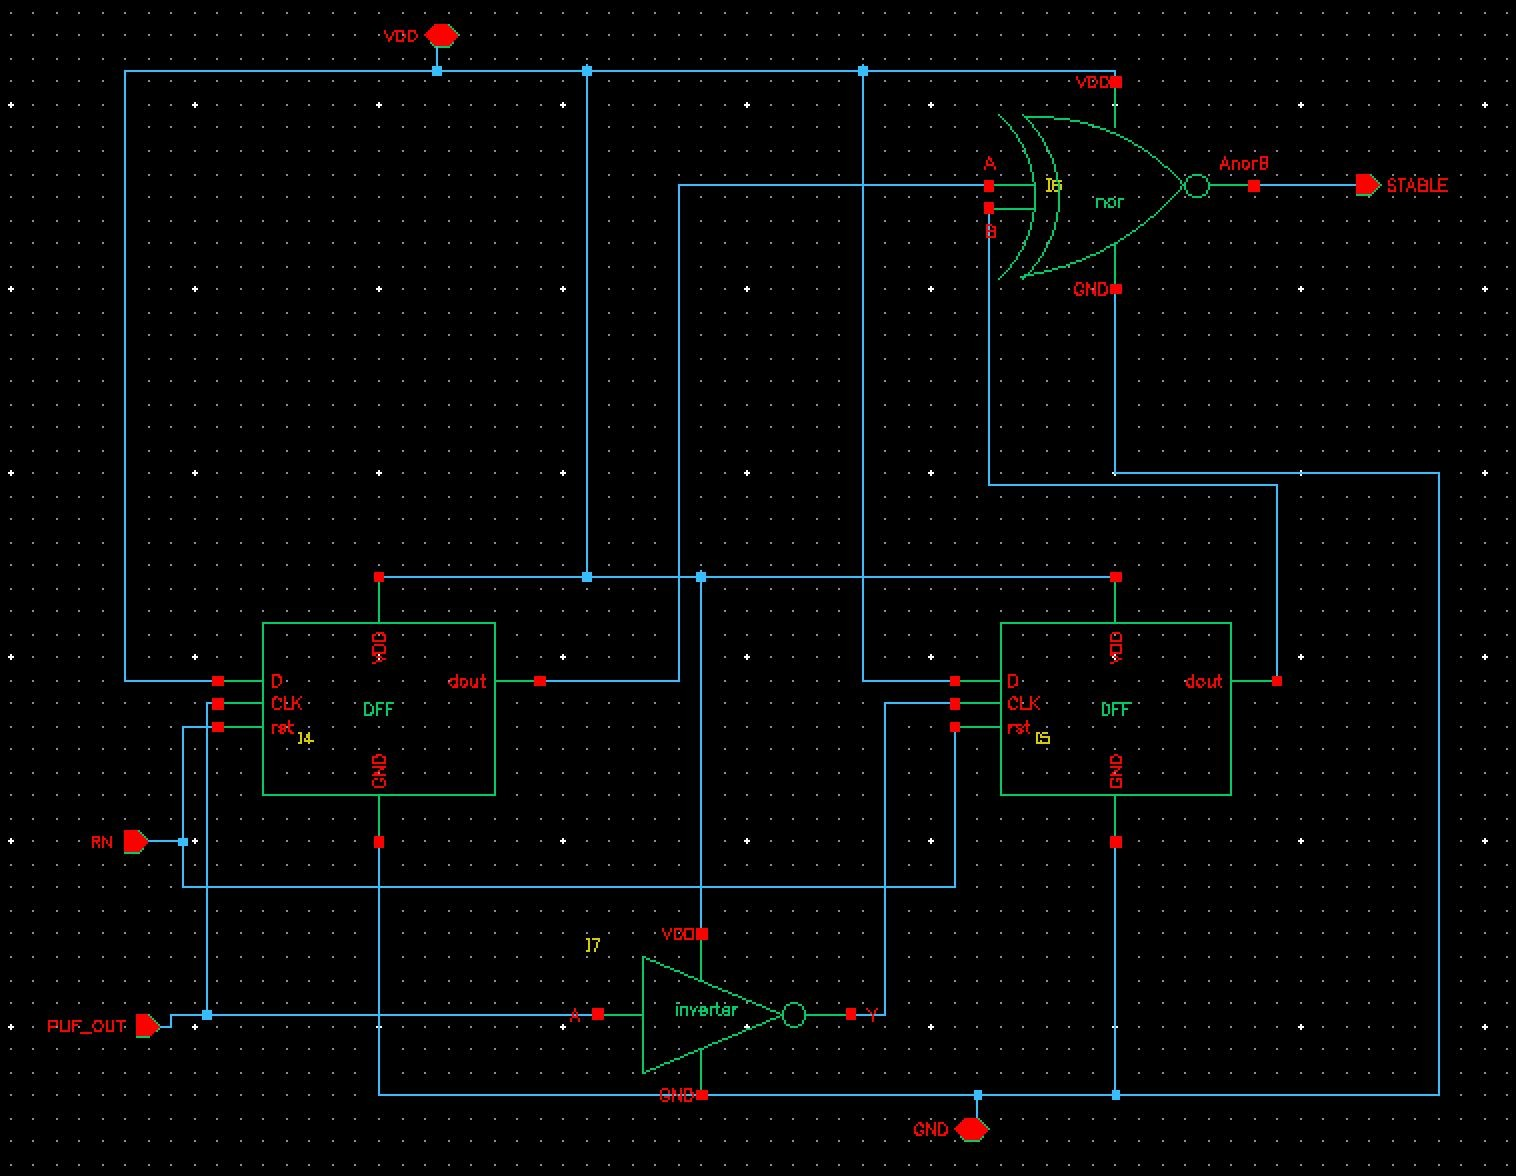
\includegraphics[width=0.92\columnwidth]{04_stability_detection.jpg}
\caption{Stability-decision circuit: two reset-able D flip-flops, an inverter and a NOR producing STABLE.}
\label{fig:stab}
\end{figure}

\begin{figure}[!t]
\centering
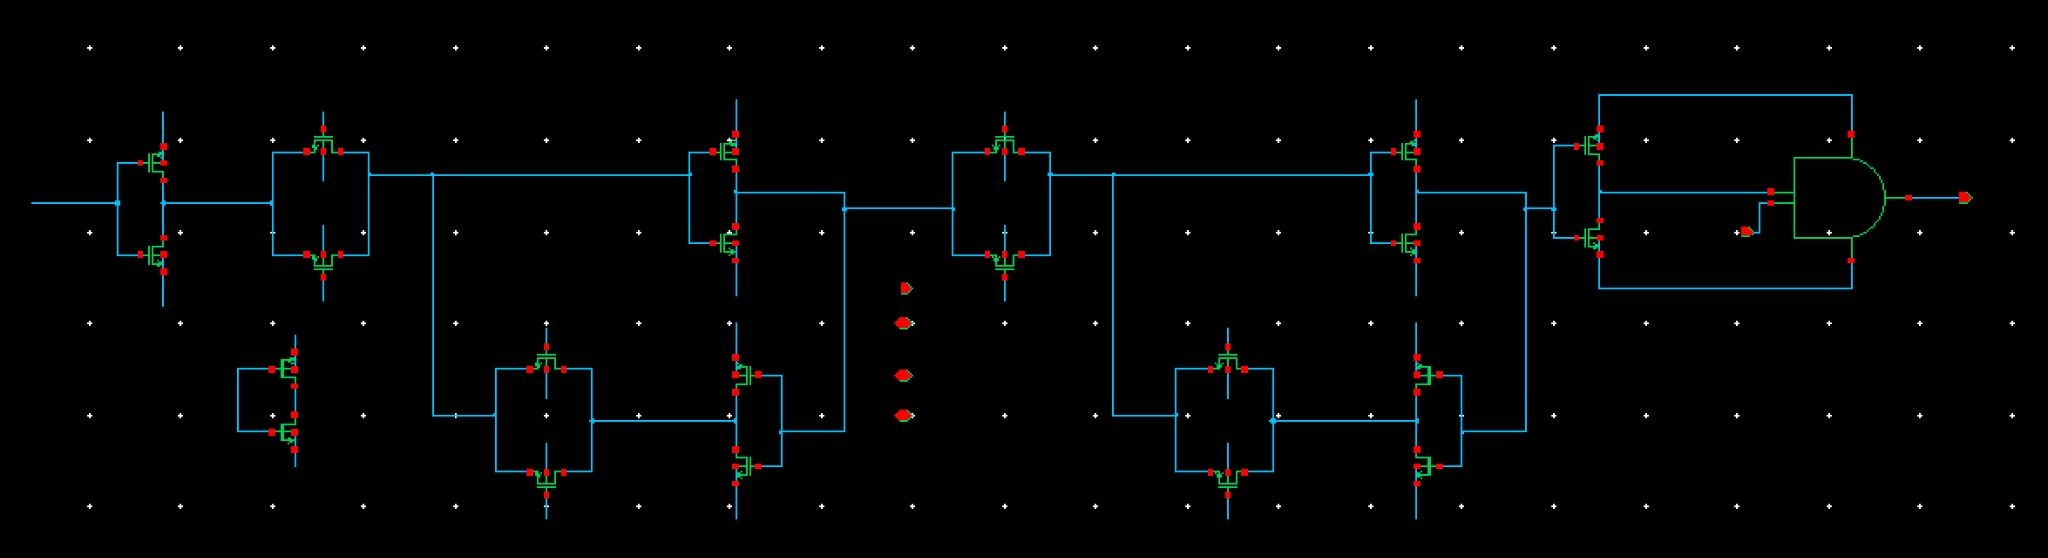
\includegraphics[width=\columnwidth]{05_dff_with_reset.jpg}
\caption{D flip-flop with active-low reset used in the readout and stability circuits.}
\label{fig:dff}
\end{figure}

\subsection{Full Array}
Fig.~\ref{fig:array} shows the complete 16$\times$16 array schematic and four zoomed regions.

\begin{figure*}[!t]
\centering
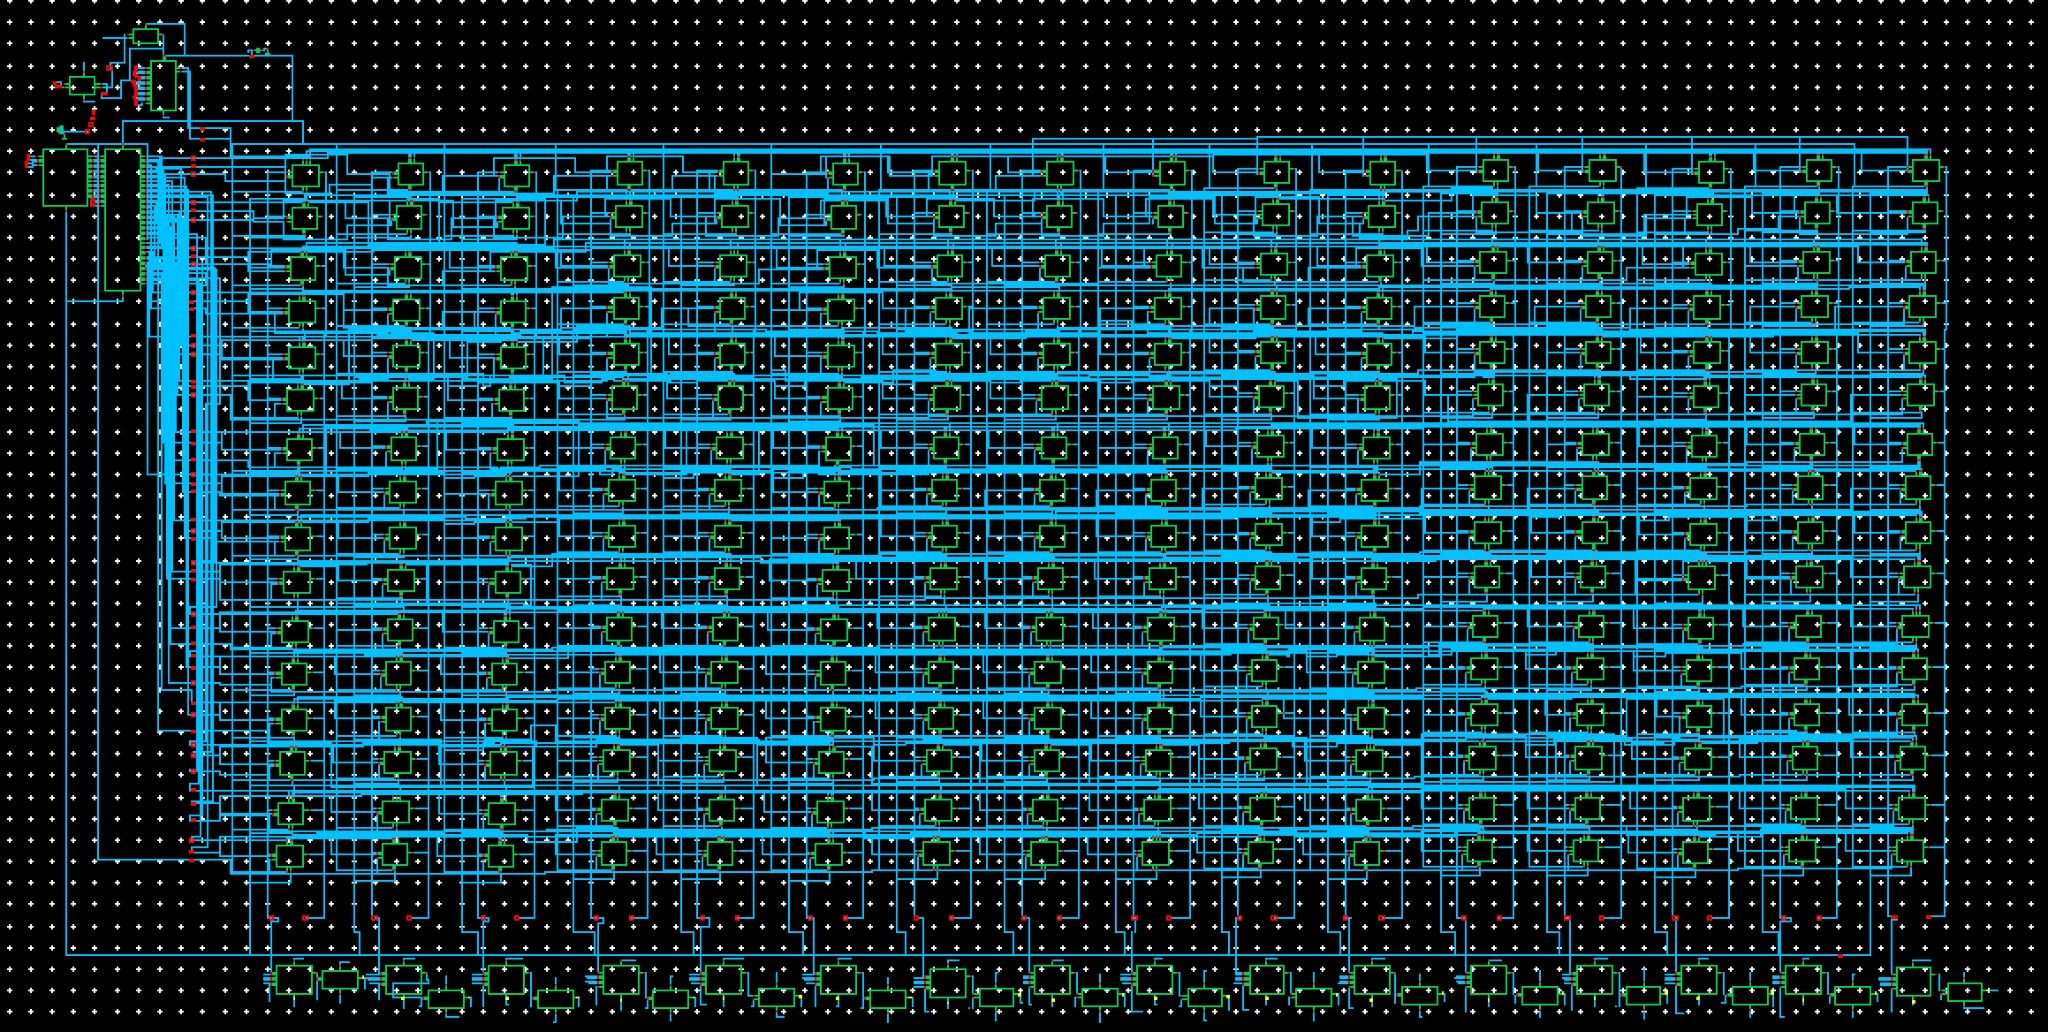
\includegraphics[width=0.62\textwidth]{02_array_16x16_full.jpg}\\[3pt]
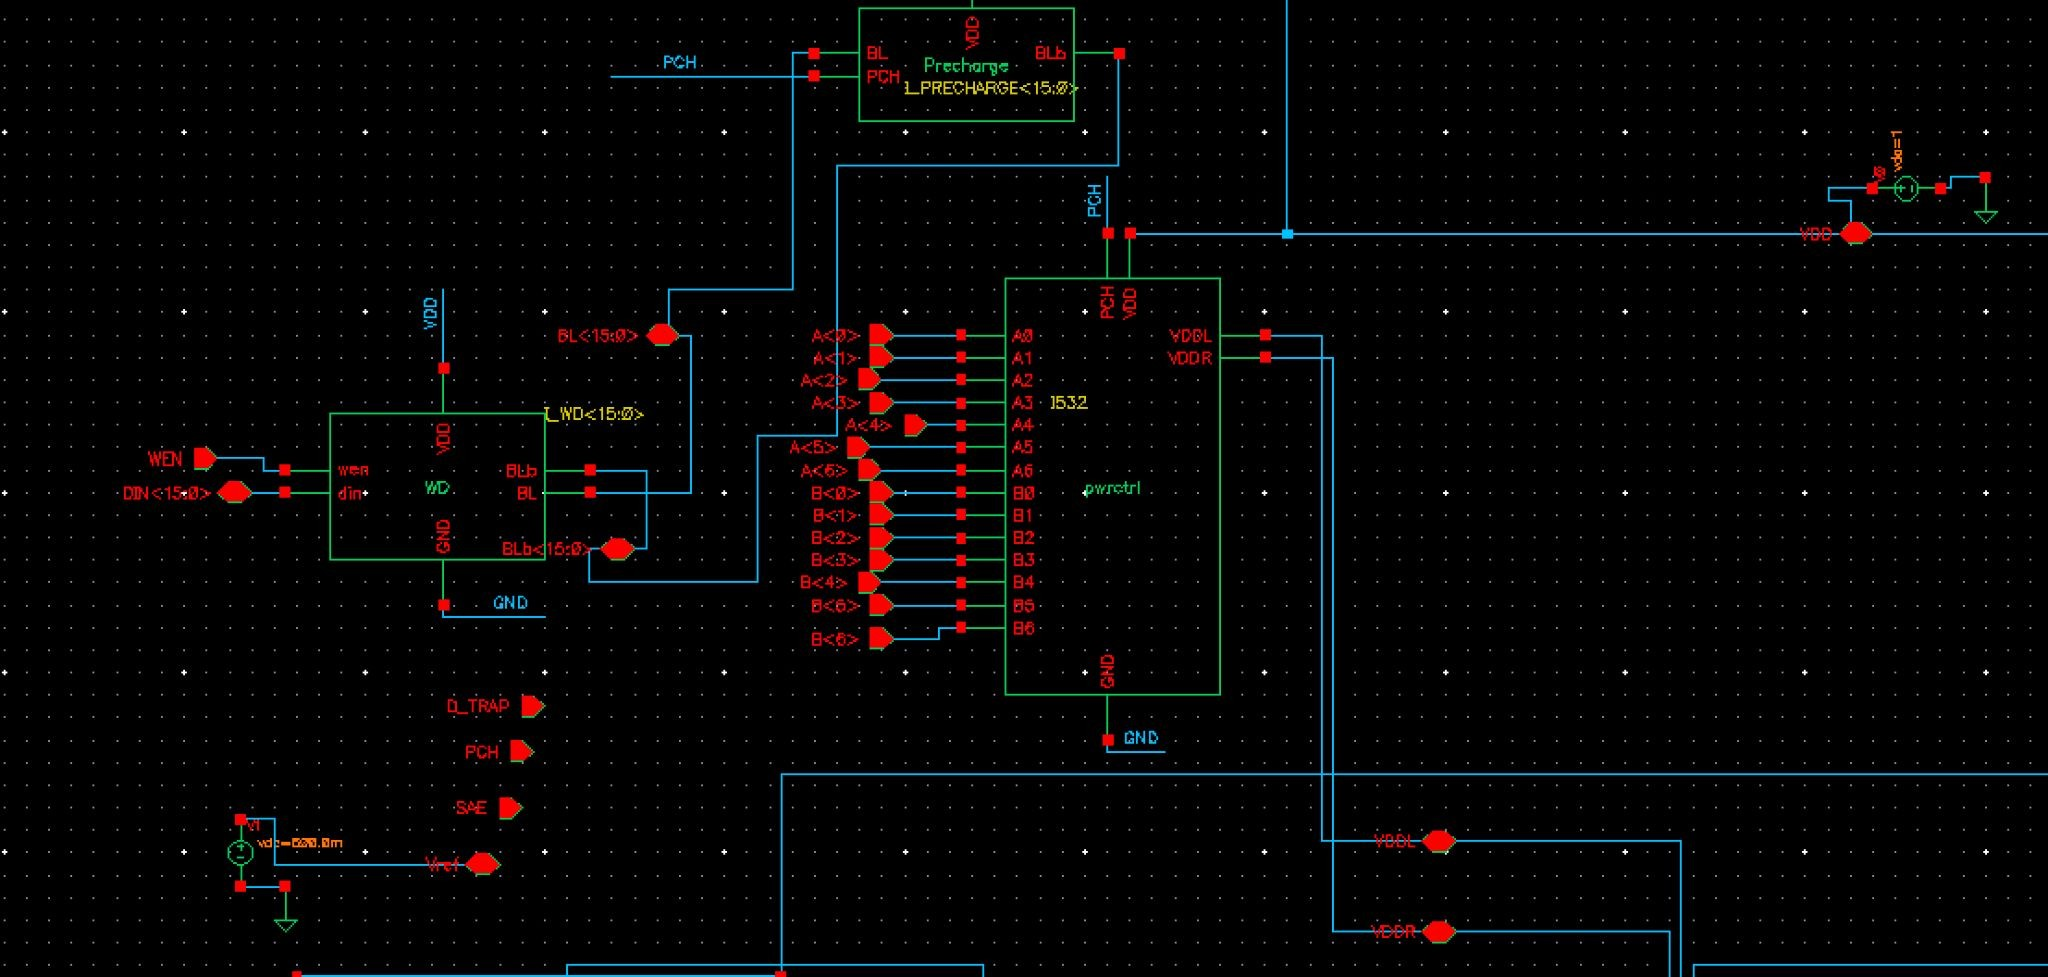
\includegraphics[width=0.24\textwidth]{03_array_16x16_zoom1.jpg}\hfill
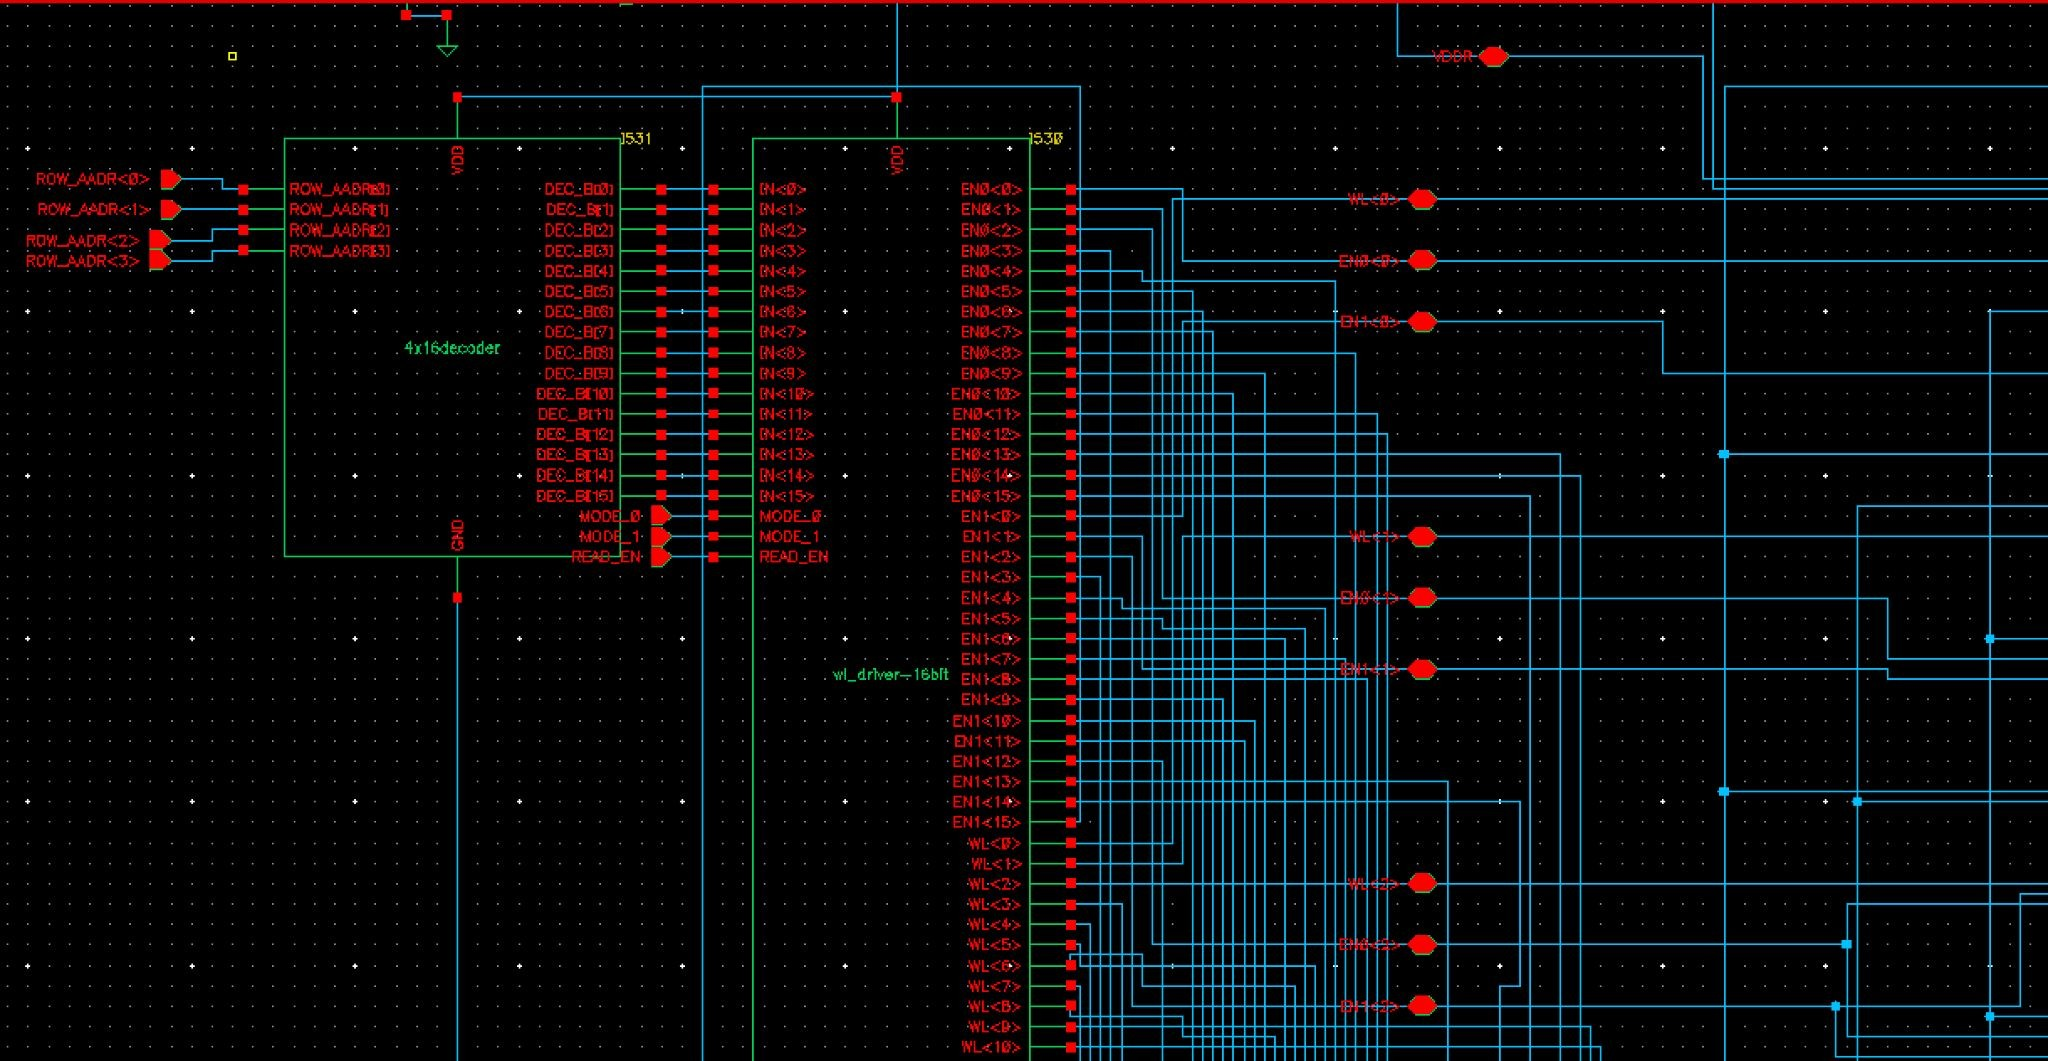
\includegraphics[width=0.24\textwidth]{04_array_16x16_zoom2.jpg}\hfill
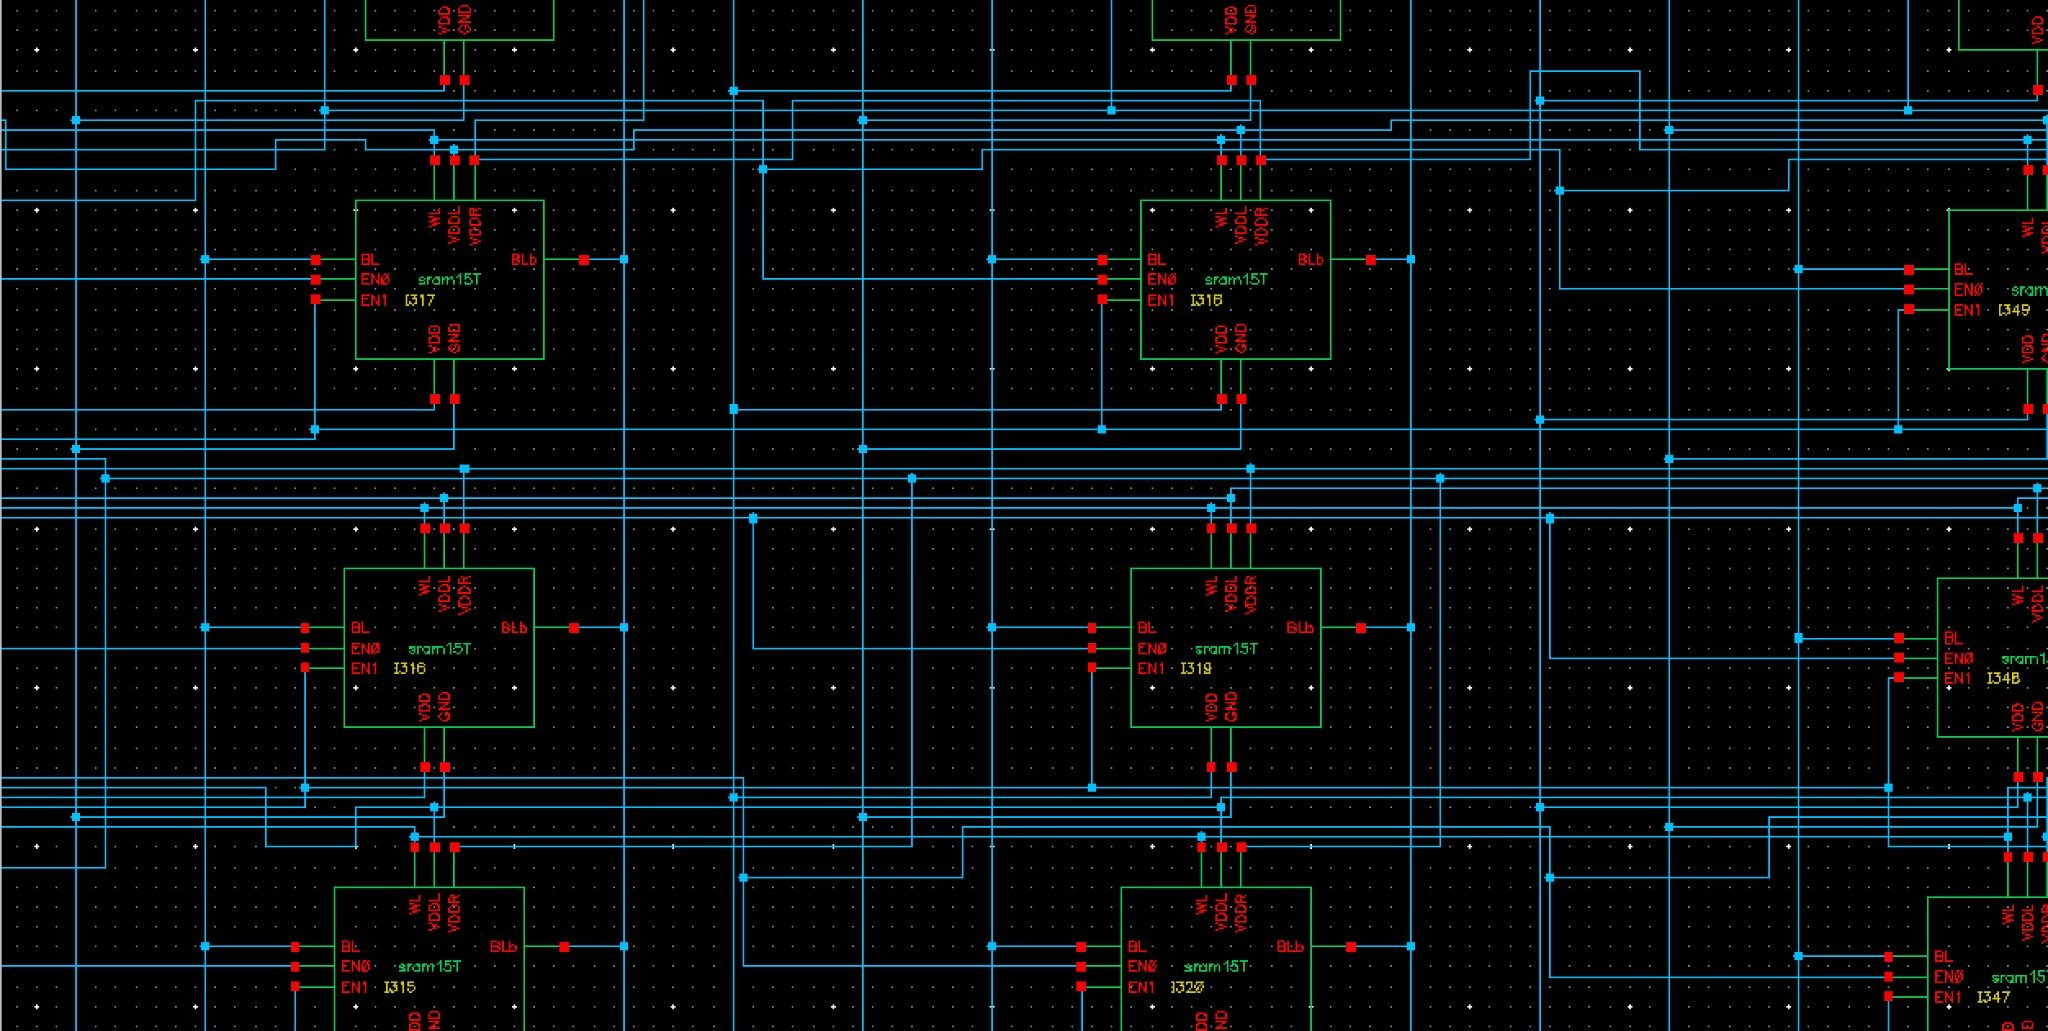
\includegraphics[width=0.24\textwidth]{05_array_16x16_zoom3.jpg}\hfill
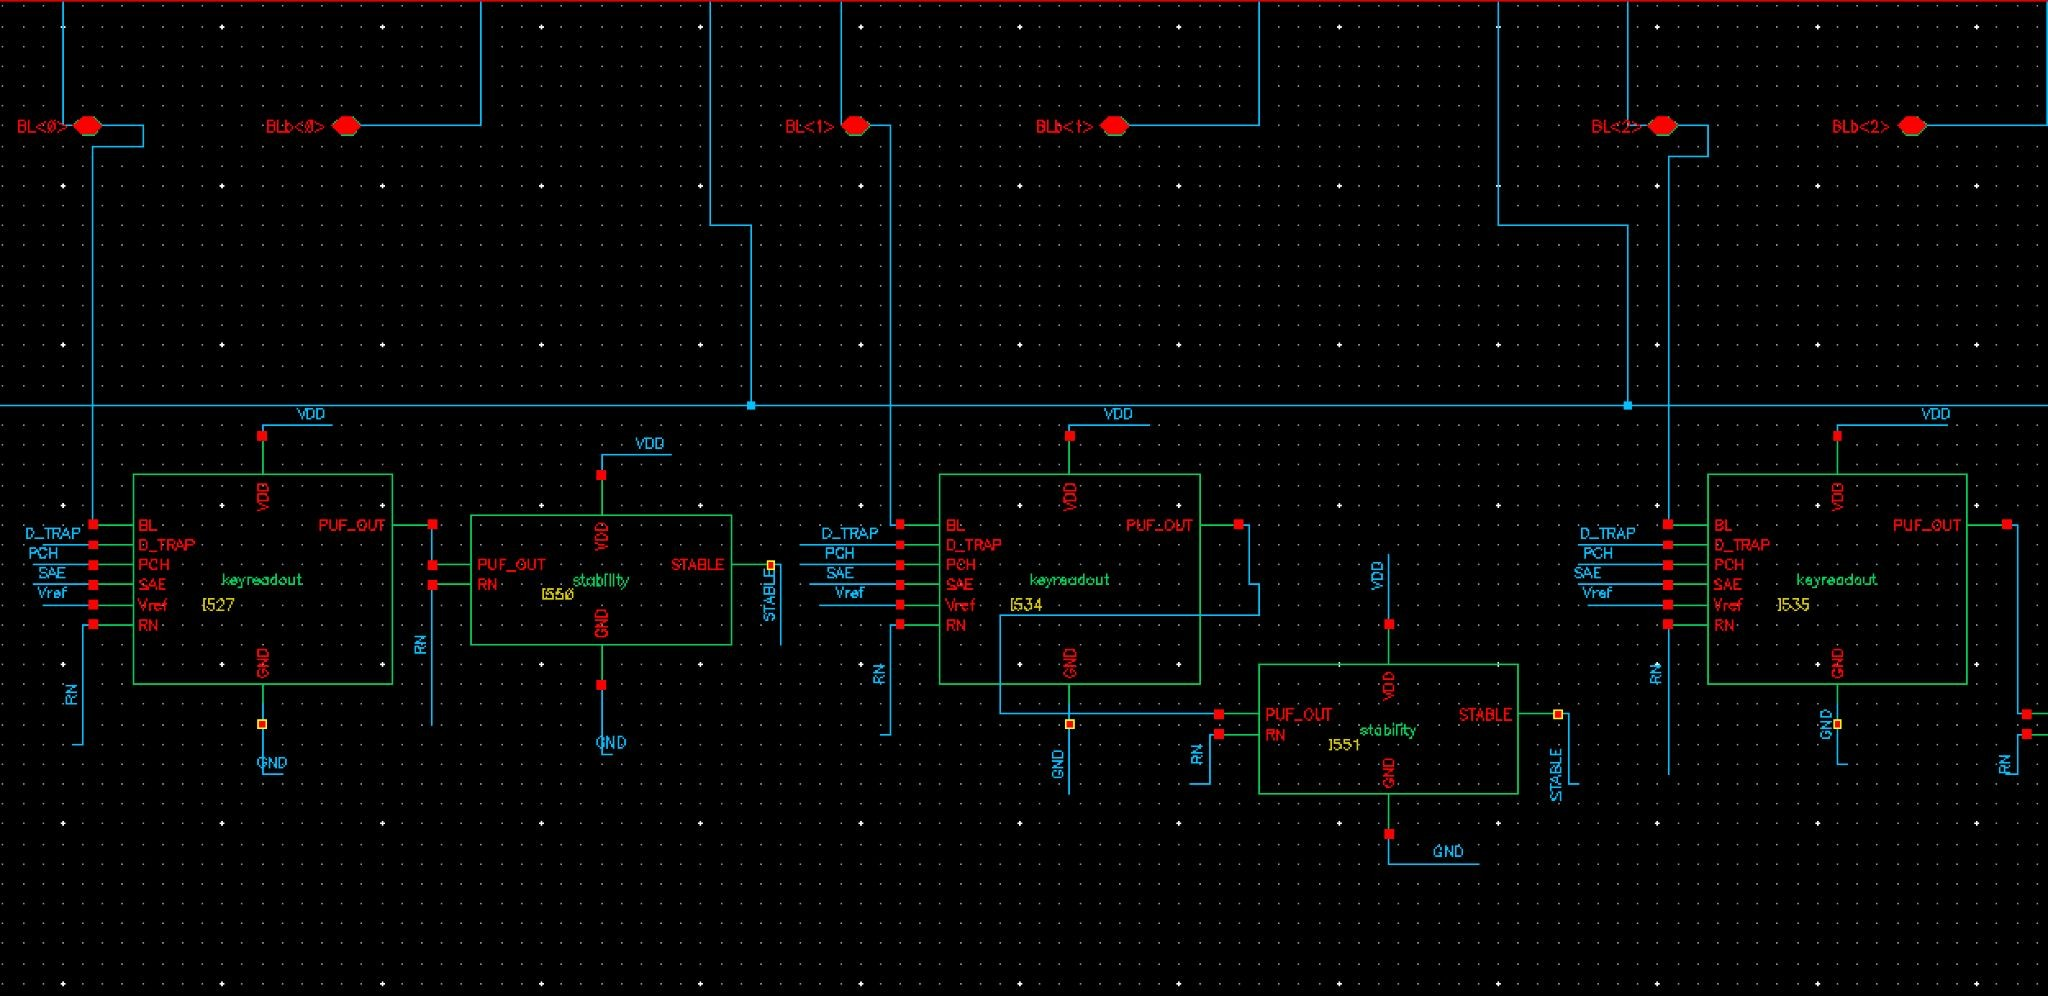
\includegraphics[width=0.24\textwidth]{06_array_16x16_zoom4.jpg}
\caption{Top: complete 16$\times$16 SRAM PUF array schematic. Bottom: zoomed views of the decoder and drivers, the row-control wiring, the cell array and the column peripherals.}
\label{fig:array}
\end{figure*}

\begin{figure*}[!t]
\centering
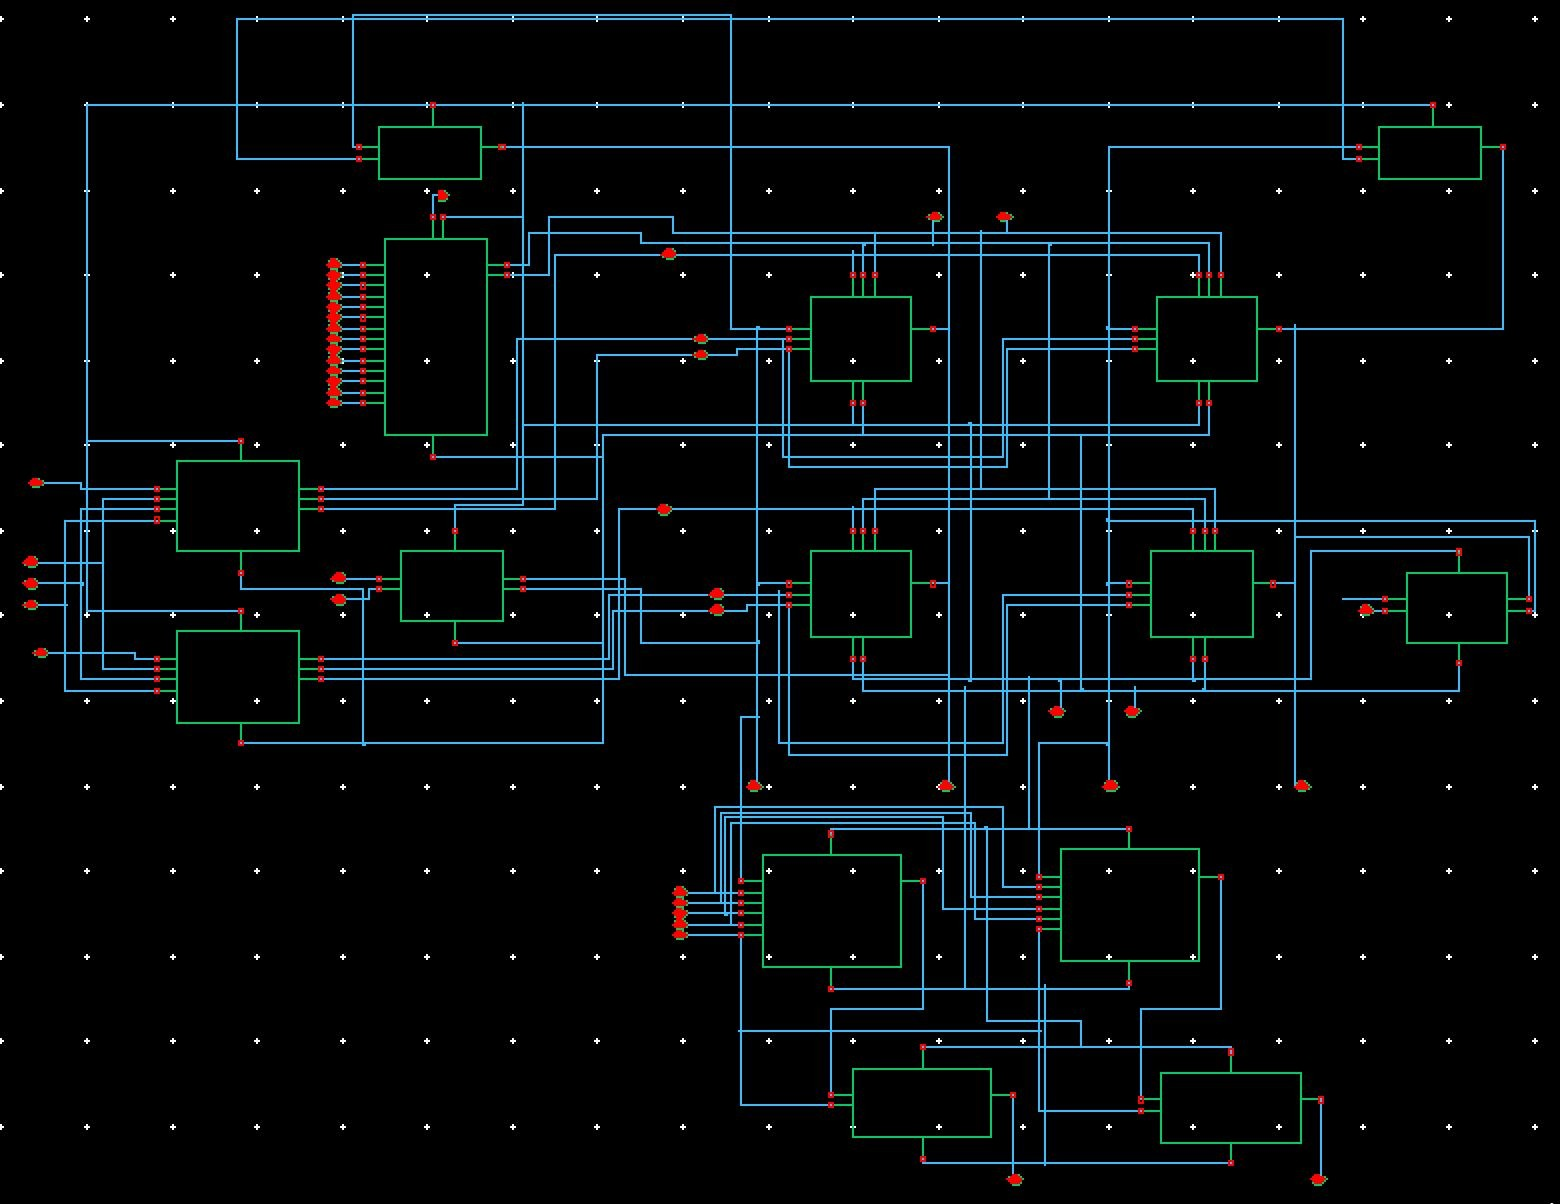
\includegraphics[width=0.40\textwidth]{07_array_2x2_test_a.jpg}\hfill
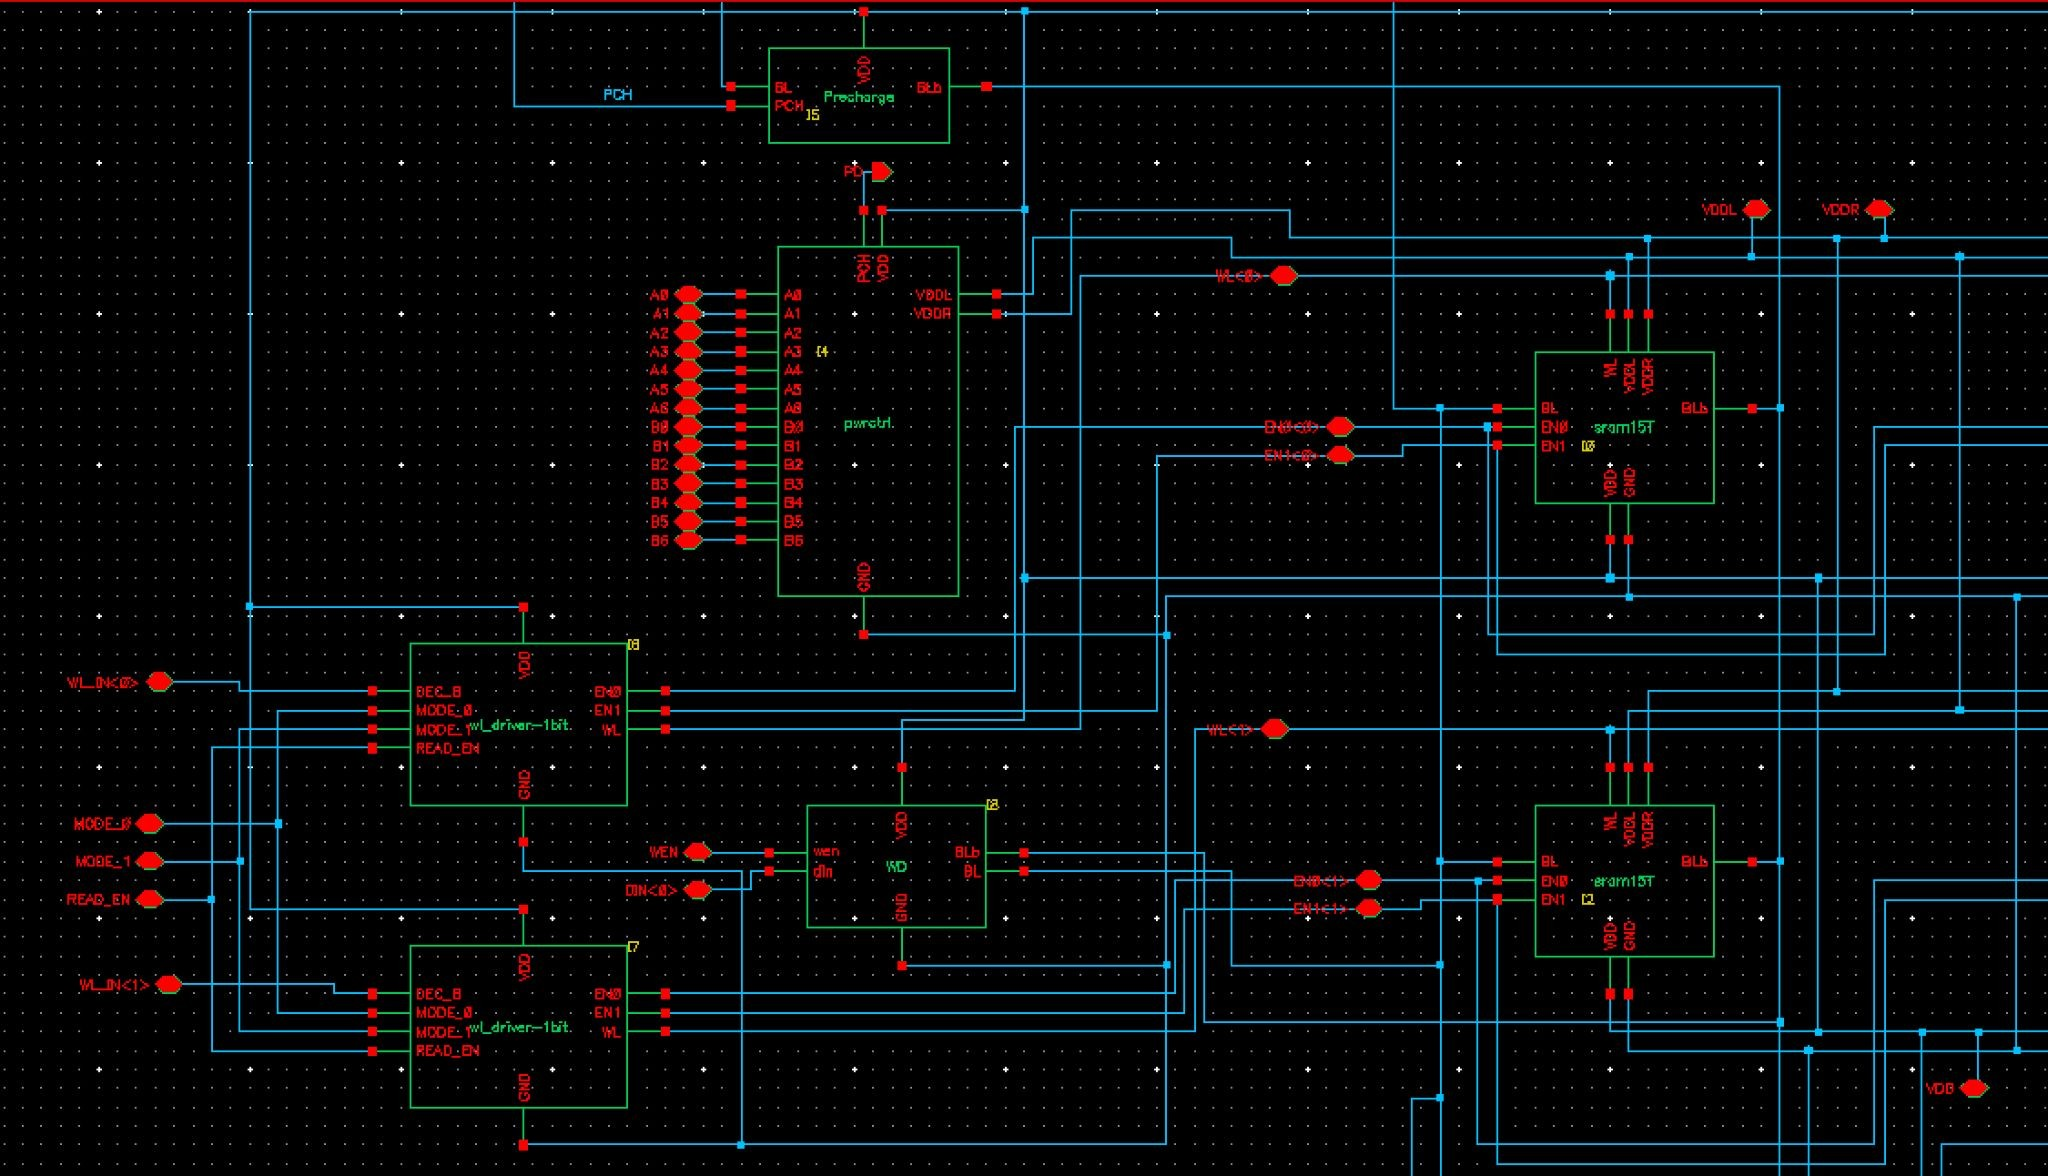
\includegraphics[width=0.27\textwidth]{08_array_2x2_test_b.jpg}\hfill
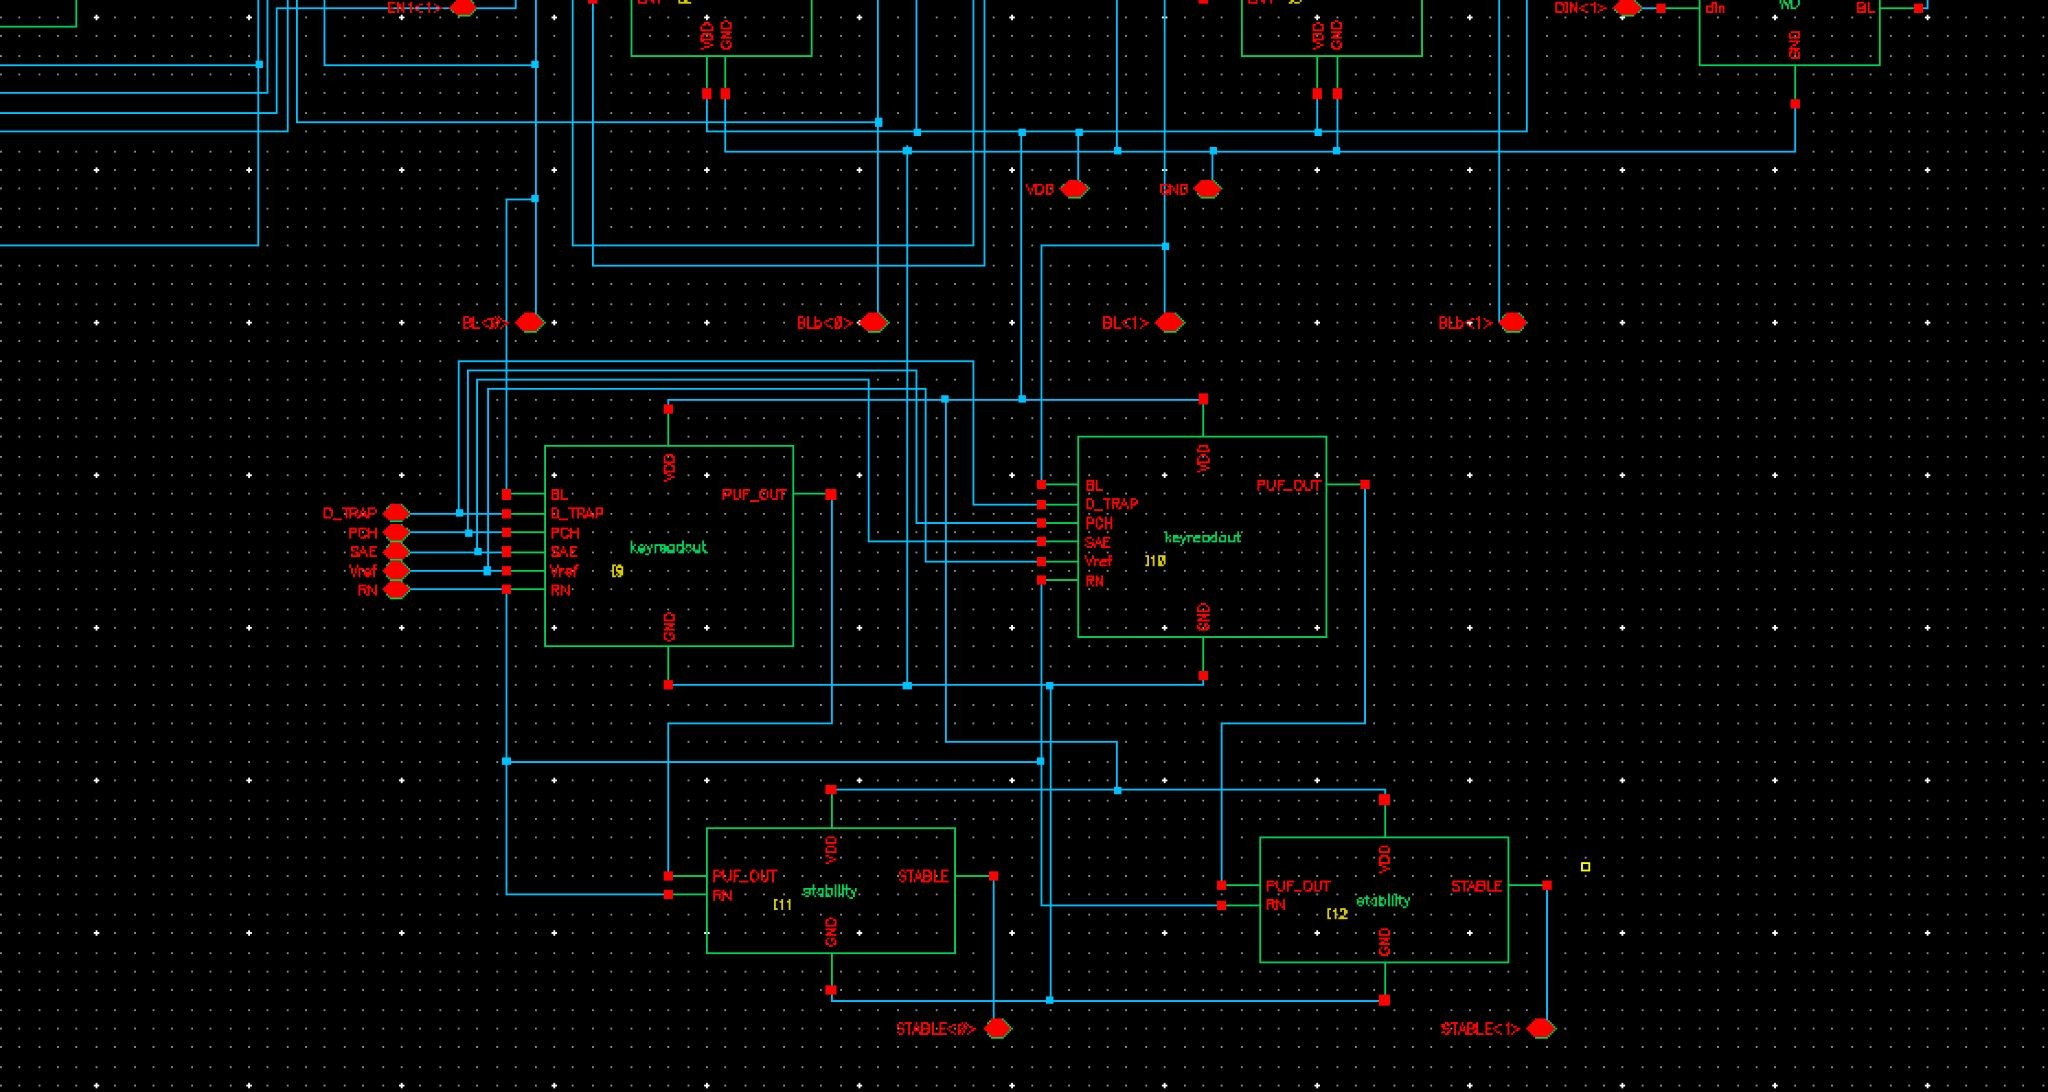
\includegraphics[width=0.27\textwidth]{09_array_2x2_test_c.jpg}\\[3pt]
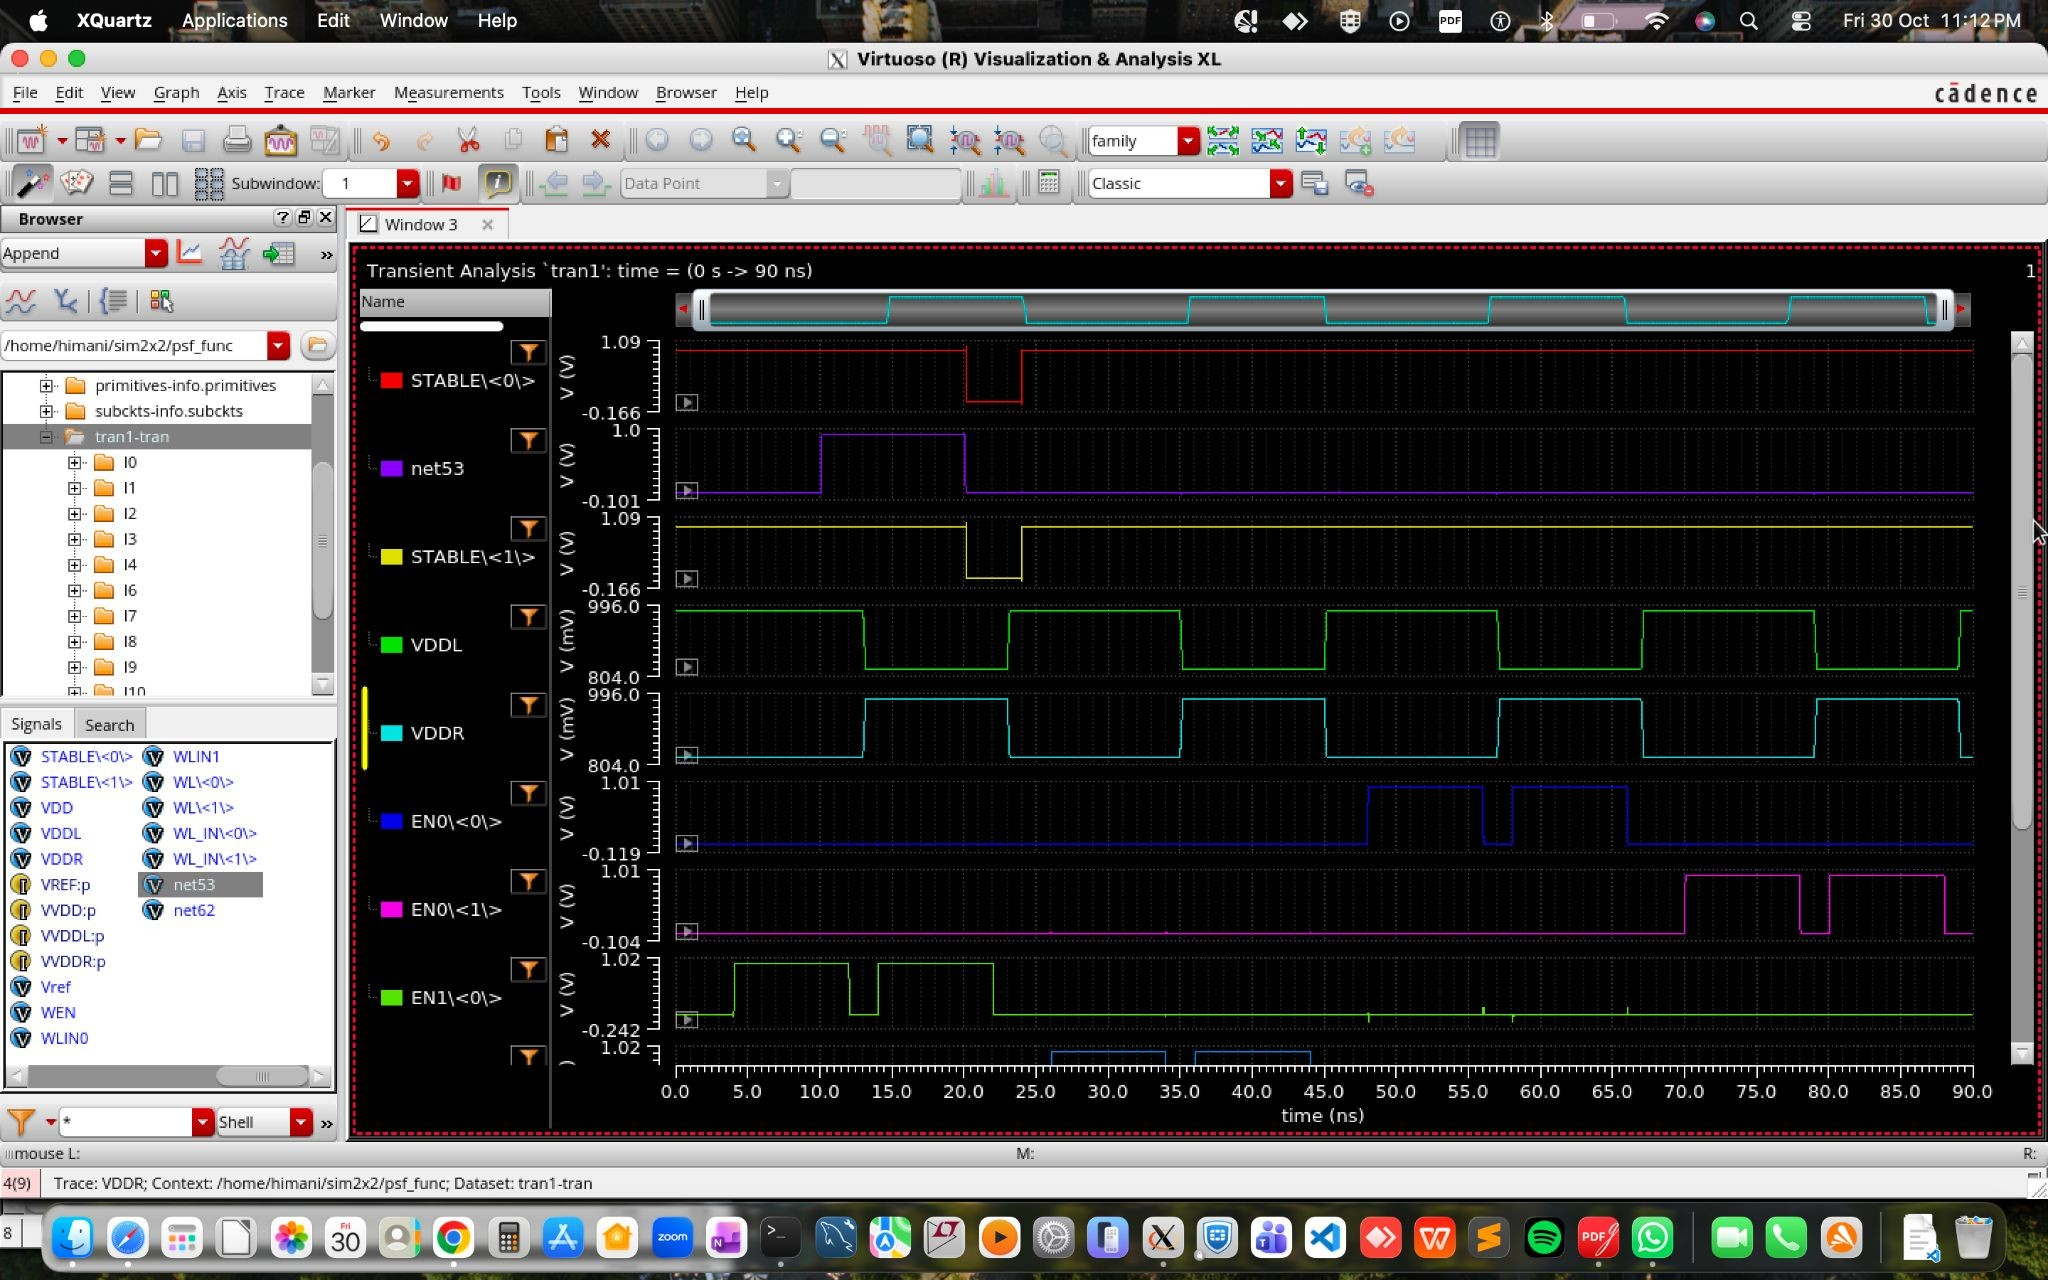
\includegraphics[width=0.49\textwidth]{04_array_2x2_transient_a.jpg}\hfill
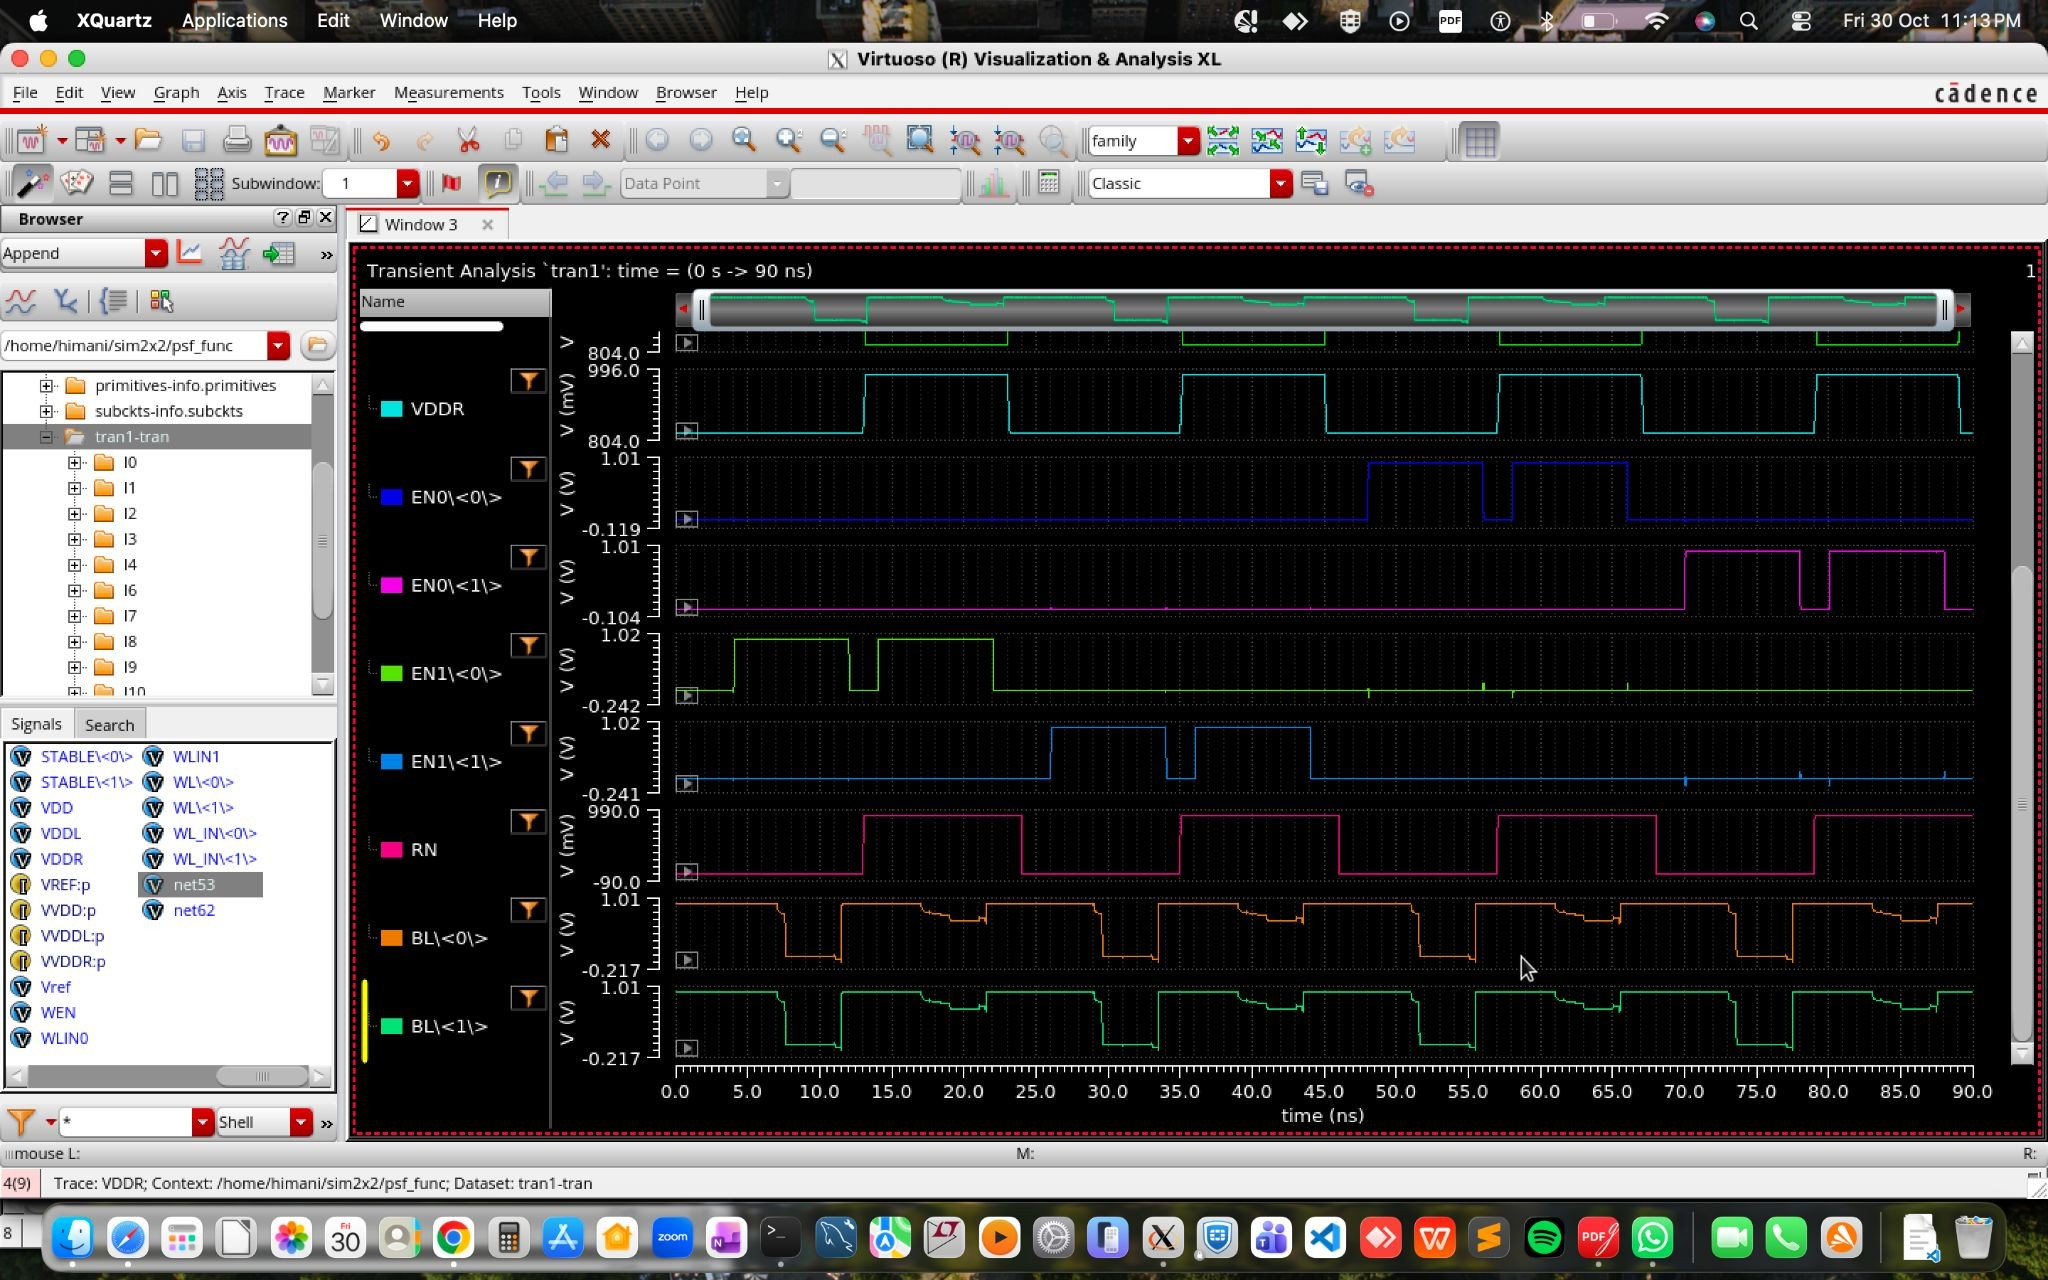
\includegraphics[width=0.49\textwidth]{05_array_2x2_transient_b.jpg}
\caption{2$\times$2 test array used to verify the integrated design. Top: schematic. Bottom: transient simulation (0--90\,ns) showing the supply rails, row enables EN0/EN1, reset RN, bitlines and the per-column STABLE outputs.}
\label{fig:2x2}
\end{figure*}

\begin{figure*}[!t]
\centering
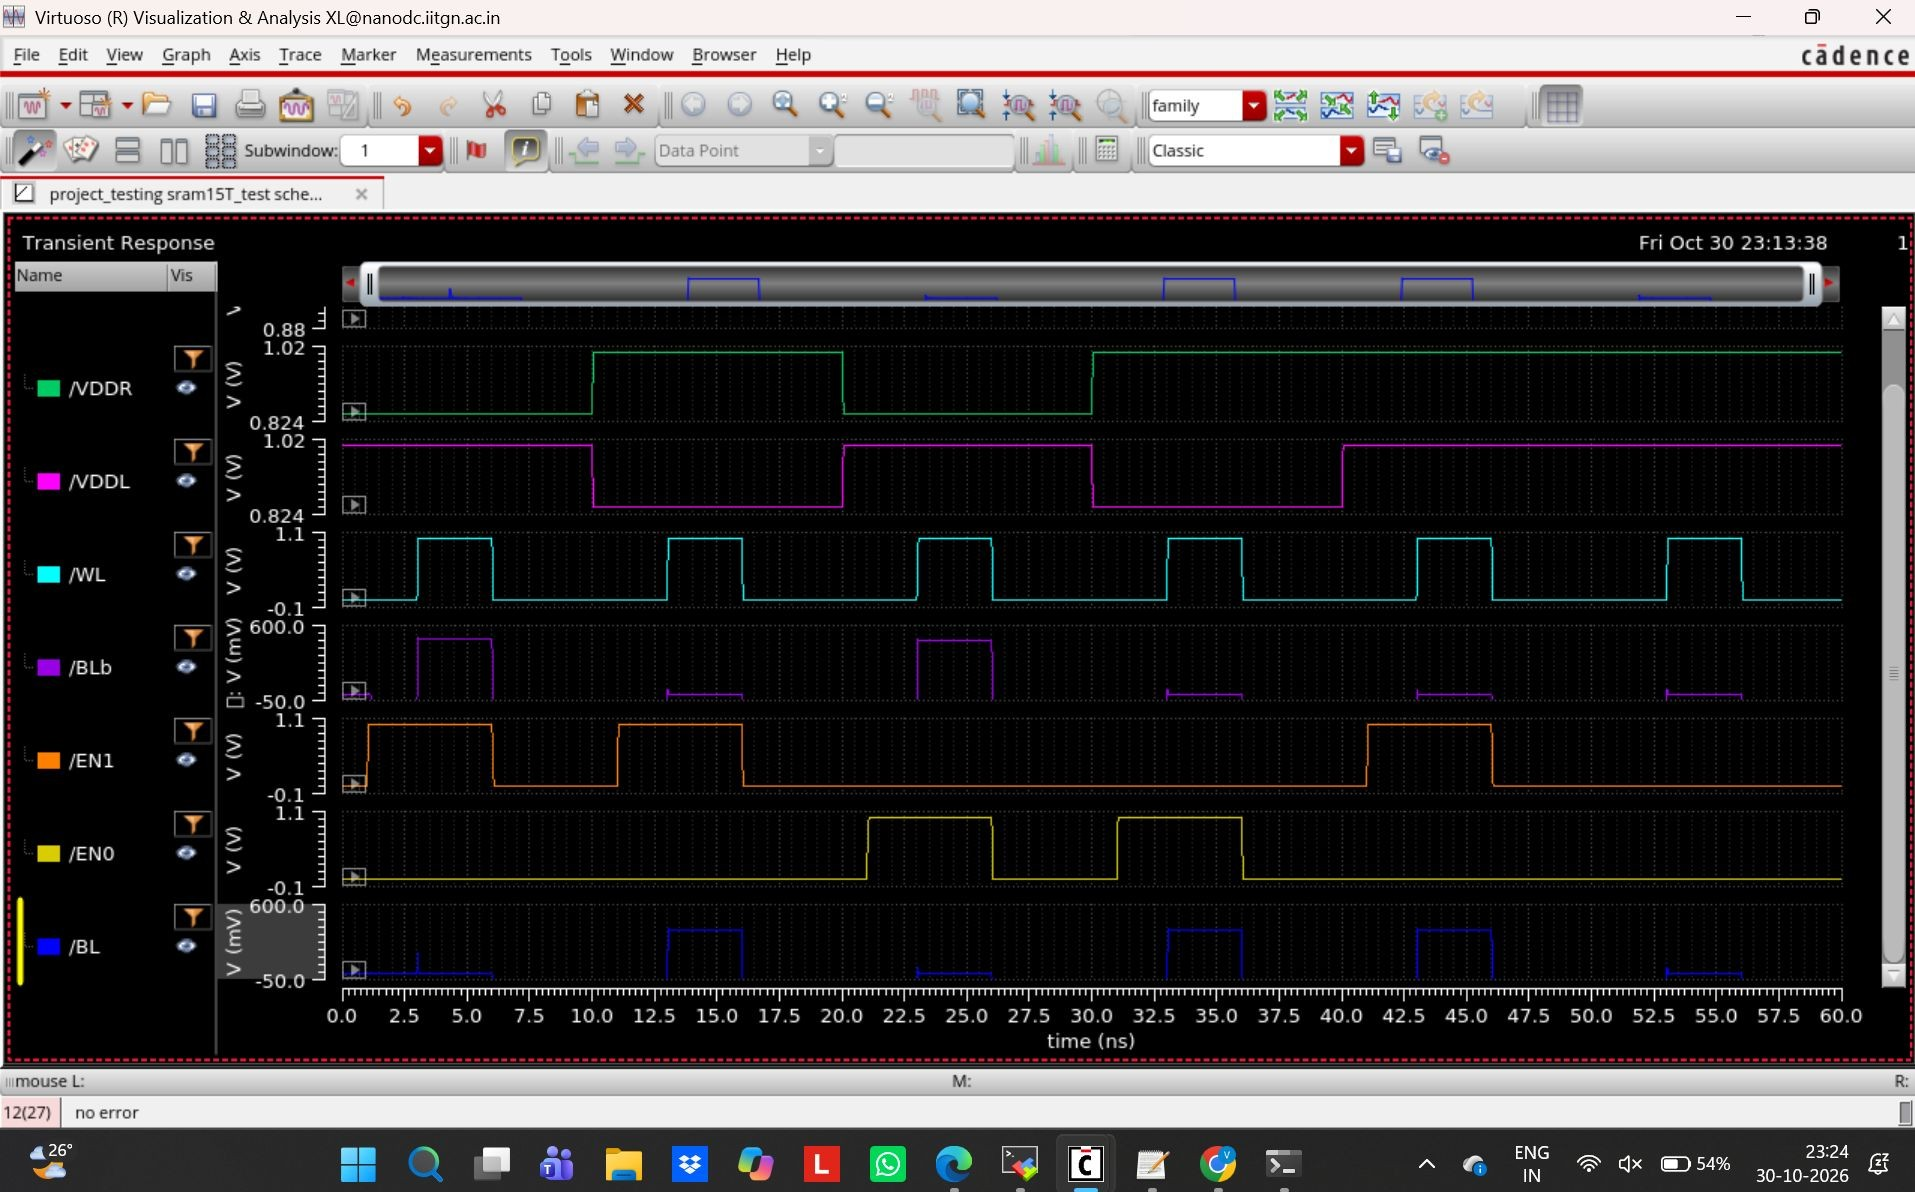
\includegraphics[width=0.49\textwidth]{01_single_cell_tilt_transient.jpg}\hfill
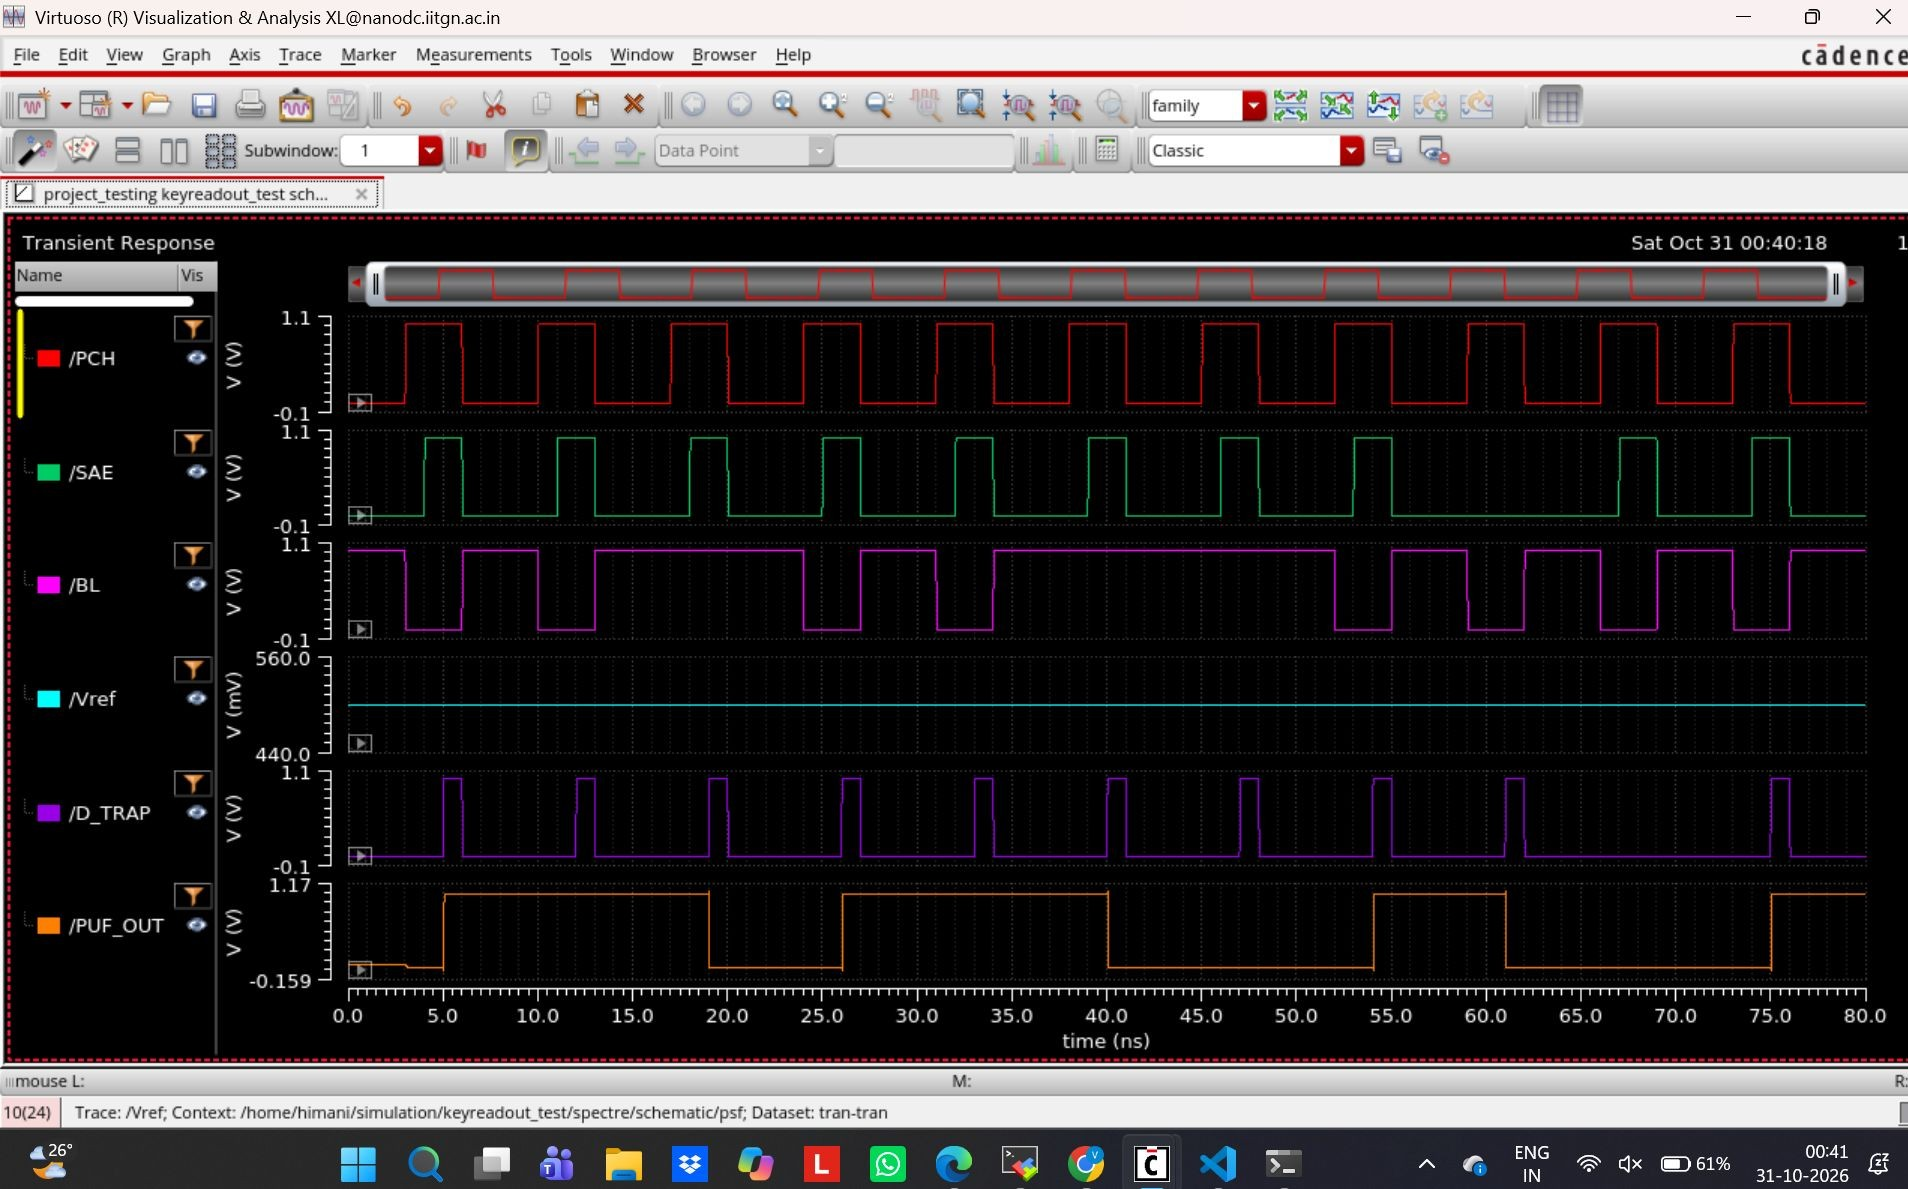
\includegraphics[width=0.49\textwidth]{02_key_readout_transient.jpg}\\[3pt]
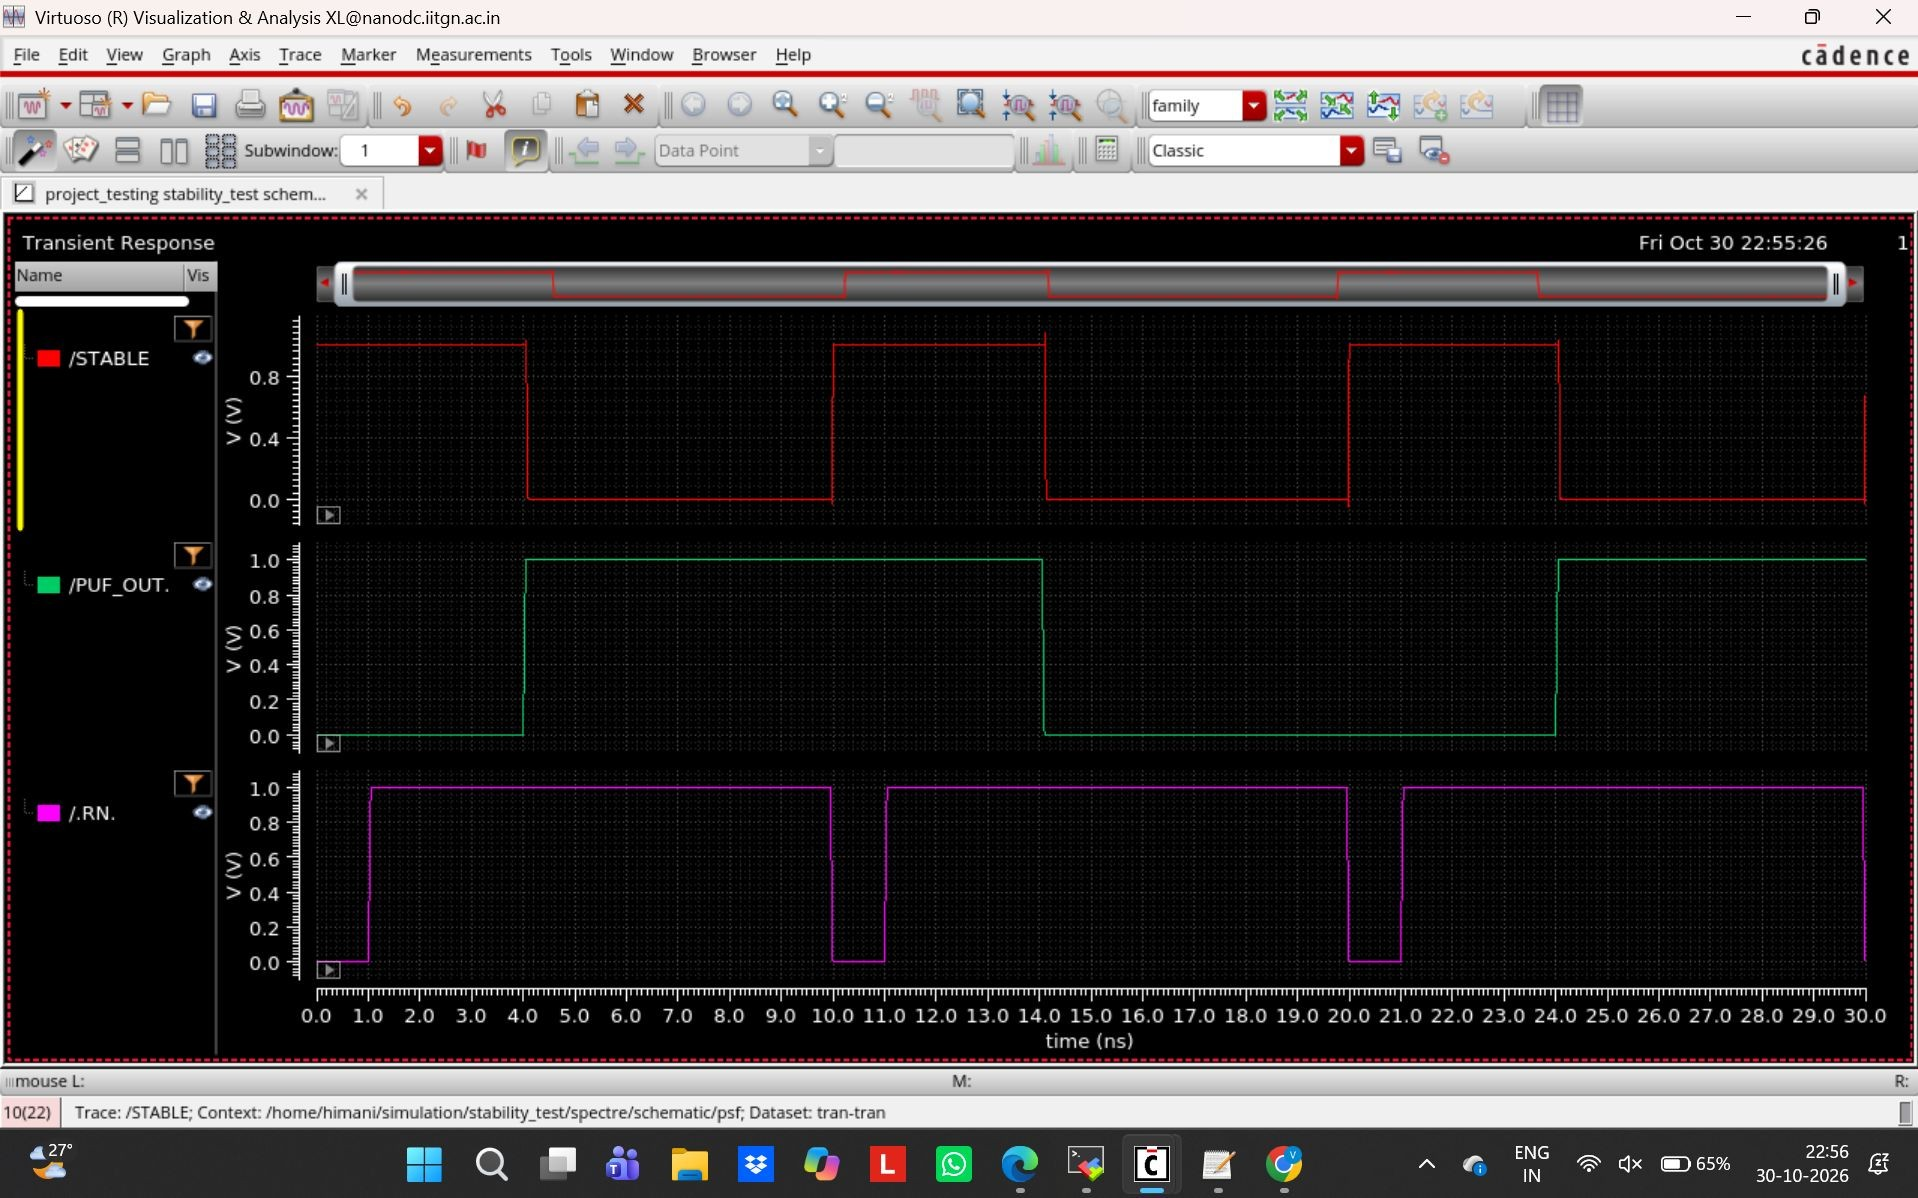
\includegraphics[width=0.49\textwidth]{03_stability_detection_transient.jpg}\hfill
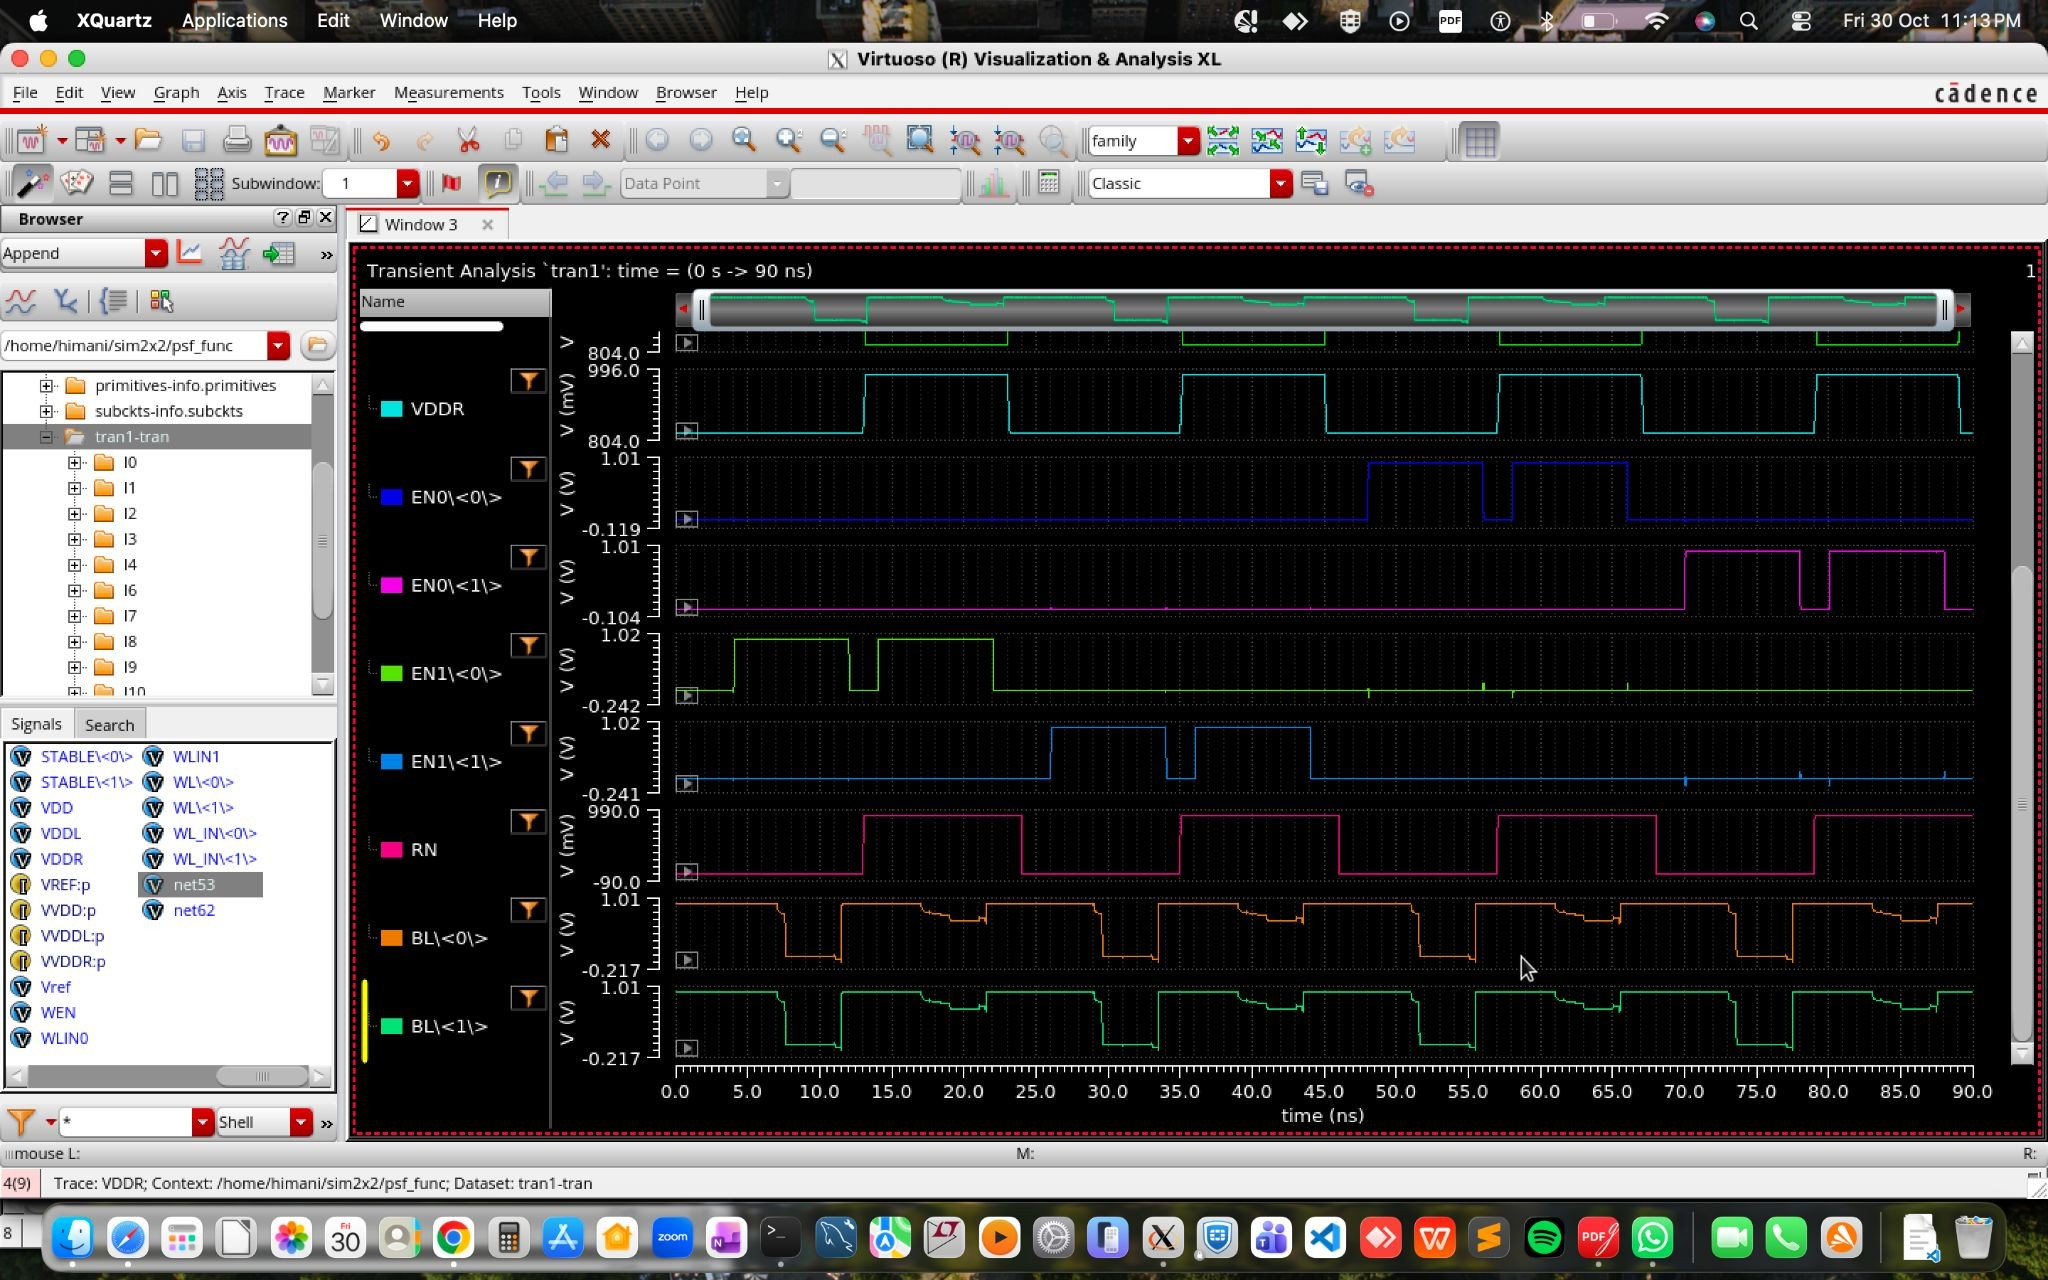
\includegraphics[width=0.49\textwidth]{07_full_circuit_sanity_check.jpg}
\caption{Block-level transient simulations. Top left: single cell under voltage tilt (VDDR, VDDL, WL, BLb, EN1, EN0, BL). Top right: key readout (PCH, SAE, BL, VREF, D\_TRAP, PUF\_OUT). Bottom left: stability decision (STABLE, PUF\_OUT, RN). Bottom right: sanity check of the integrated circuit.}
\label{fig:blocksim}
\end{figure*}

\section{Functional Verification and Simulation Setup}
\subsection{Block, 2$\times$2 and 16$\times$16 Verification}
Each block was simulated on its own before integration (Fig.~\ref{fig:blocksim}). The single-cell testbench applies both tilt polarities on VDDL/VDDR and evaluates in each mode; the key-readout testbench steps through precharge, WL enable and sensing and latches PUF\_OUT on D\_TRAP; the stability testbench shows STABLE falling when PUF\_OUT changes between the two stages and being restored by RN. To test integration, a 2$\times$2 array with all peripherals was built and simulated first (Fig.~\ref{fig:2x2}), and then the full 16$\times$16 array. A nominal run of the full array without mismatch (Fig.~\ref{fig:verify}, left; ten evaluations, temporal majority voting over three repeats) confirms that all 256 cells respond: every cell resolves, no cell is flagged unstable, and, as expected without mismatch, all cells settle to the same value. Monte Carlo analysis of the array was then set up in ADE Explorer (Fig.~\ref{fig:verify}, right), probing PUF\_OUT and STABLE for all sixteen columns.

\begin{figure}[!t]
\centering
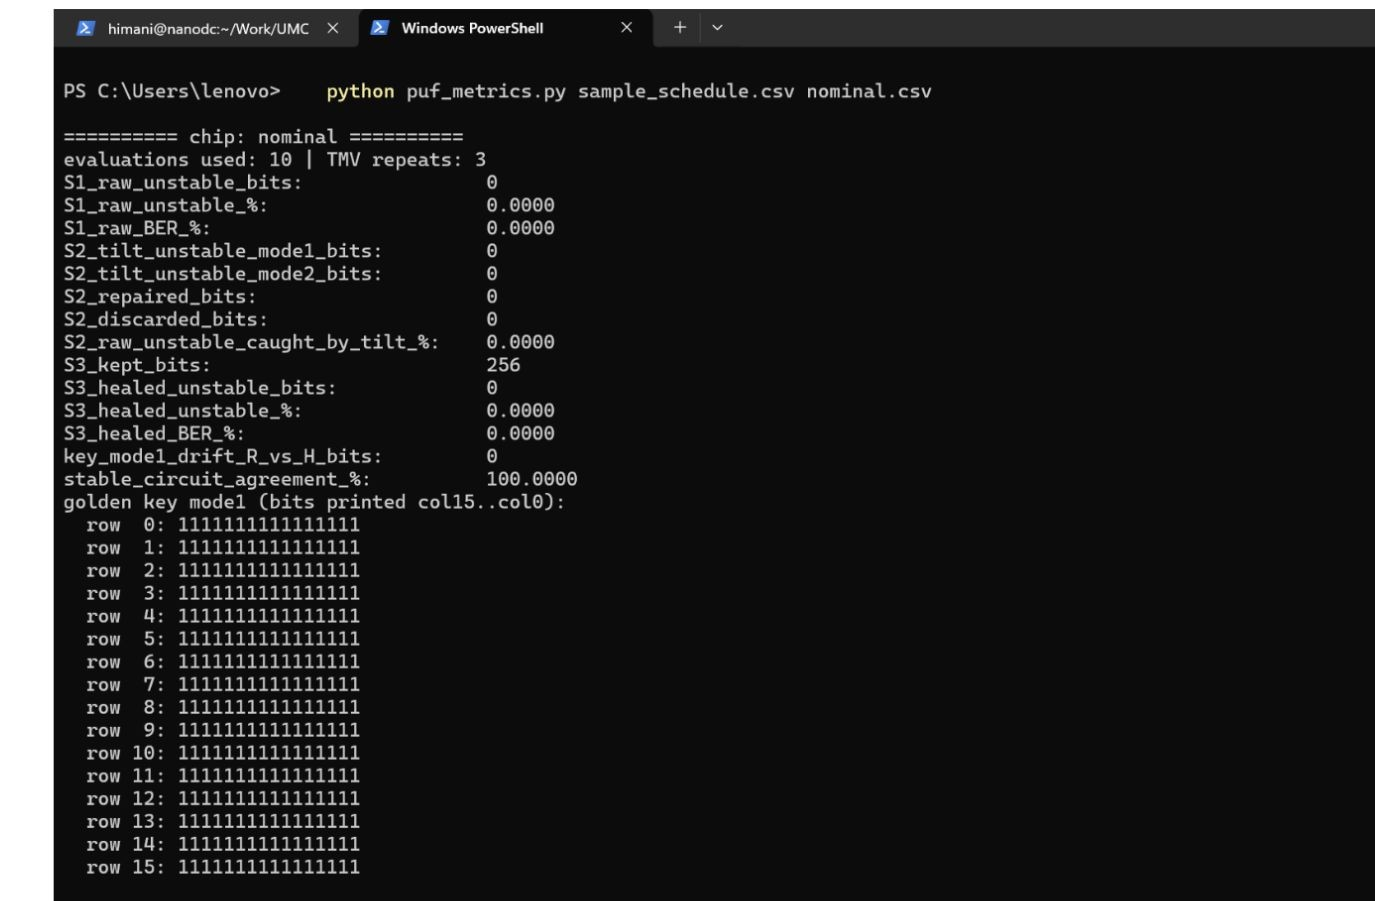
\includegraphics[width=0.49\columnwidth]{06_array_16x16_nominal_verification.jpg}\hfill
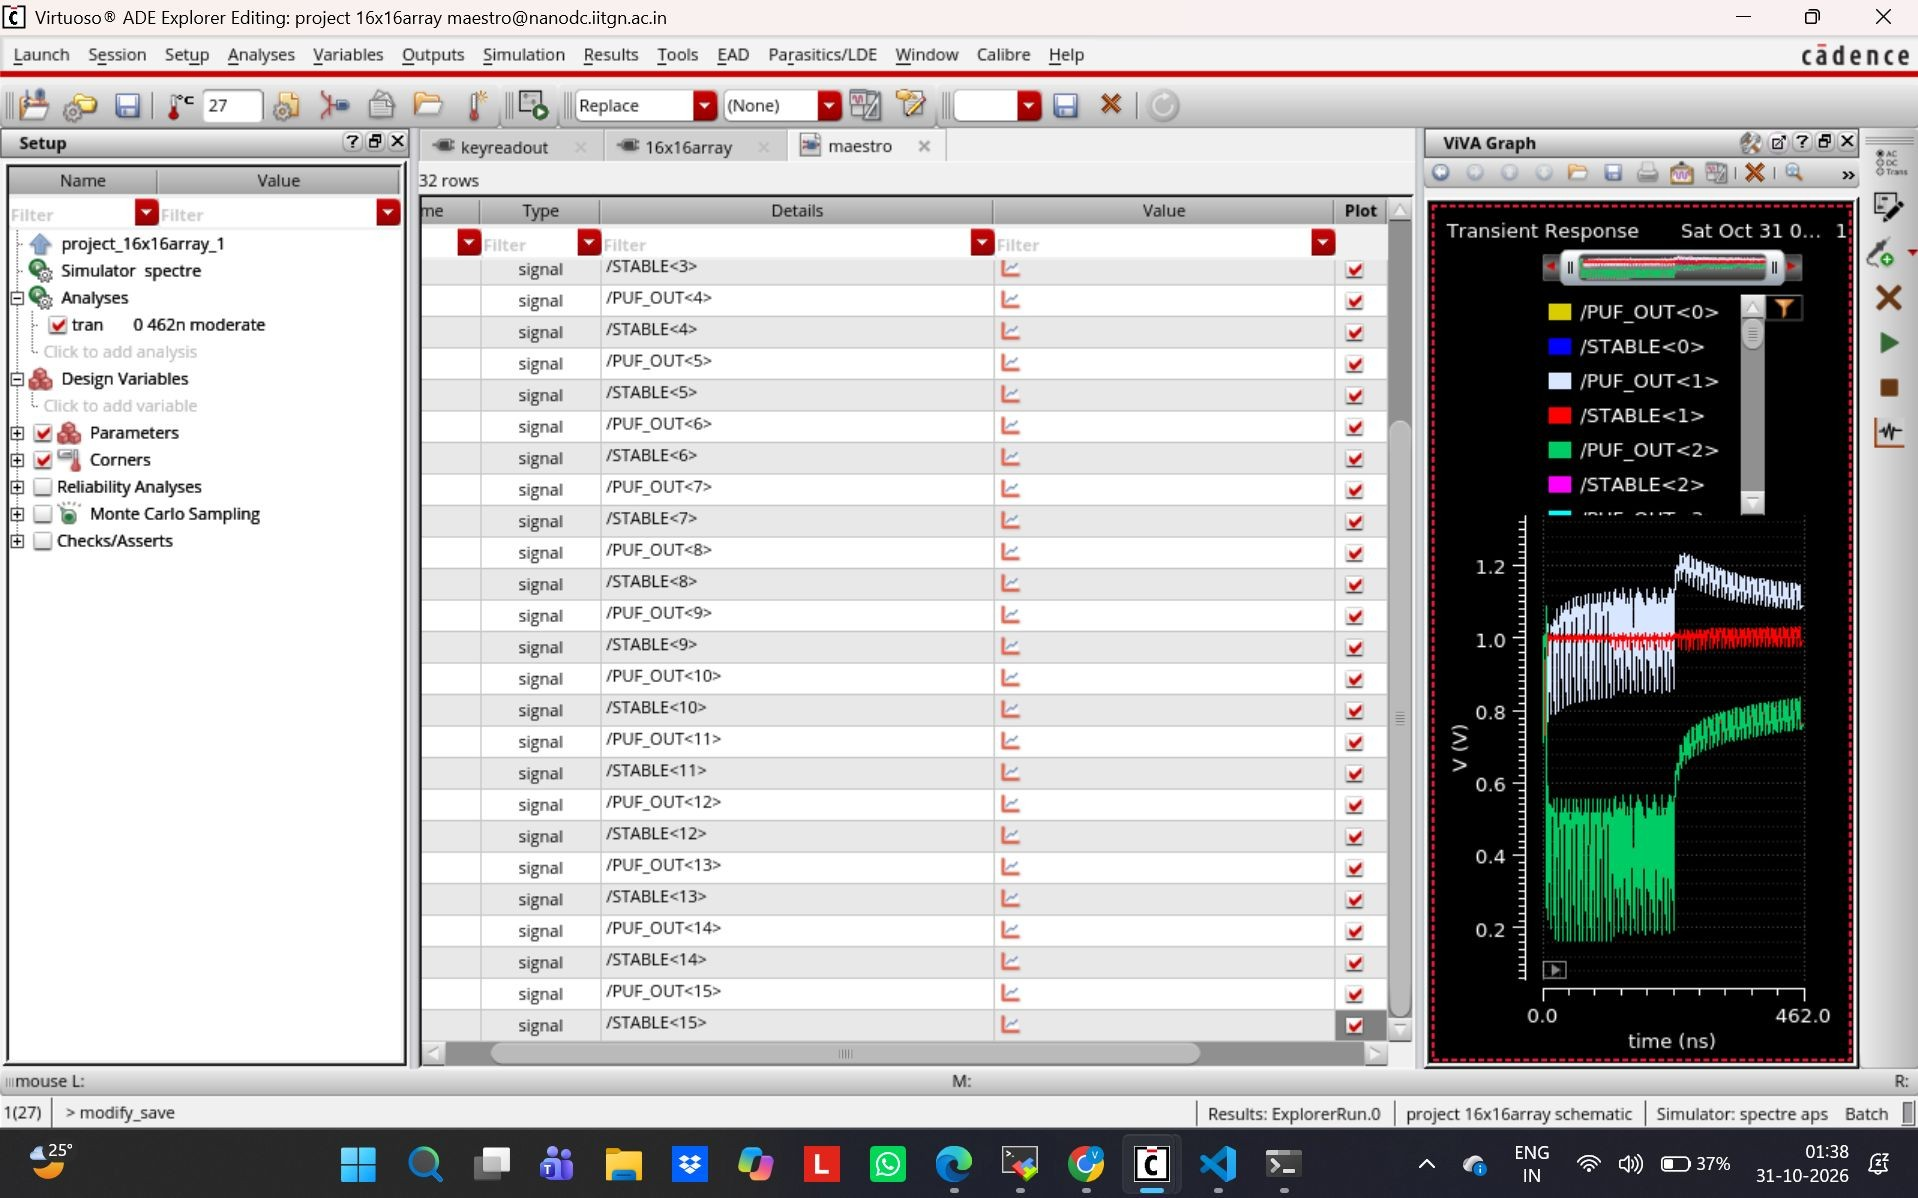
\includegraphics[width=0.49\columnwidth]{08_monte_carlo_setup_maestro.jpg}
\caption{Left: nominal verification of the 16$\times$16 array; all 256 cells respond and none is flagged unstable. Right: Monte Carlo setup in ADE Explorer (Maestro) for the 16$\times$16 array.}
\label{fig:verify}
\end{figure}

\begin{figure*}[!t]
\centering
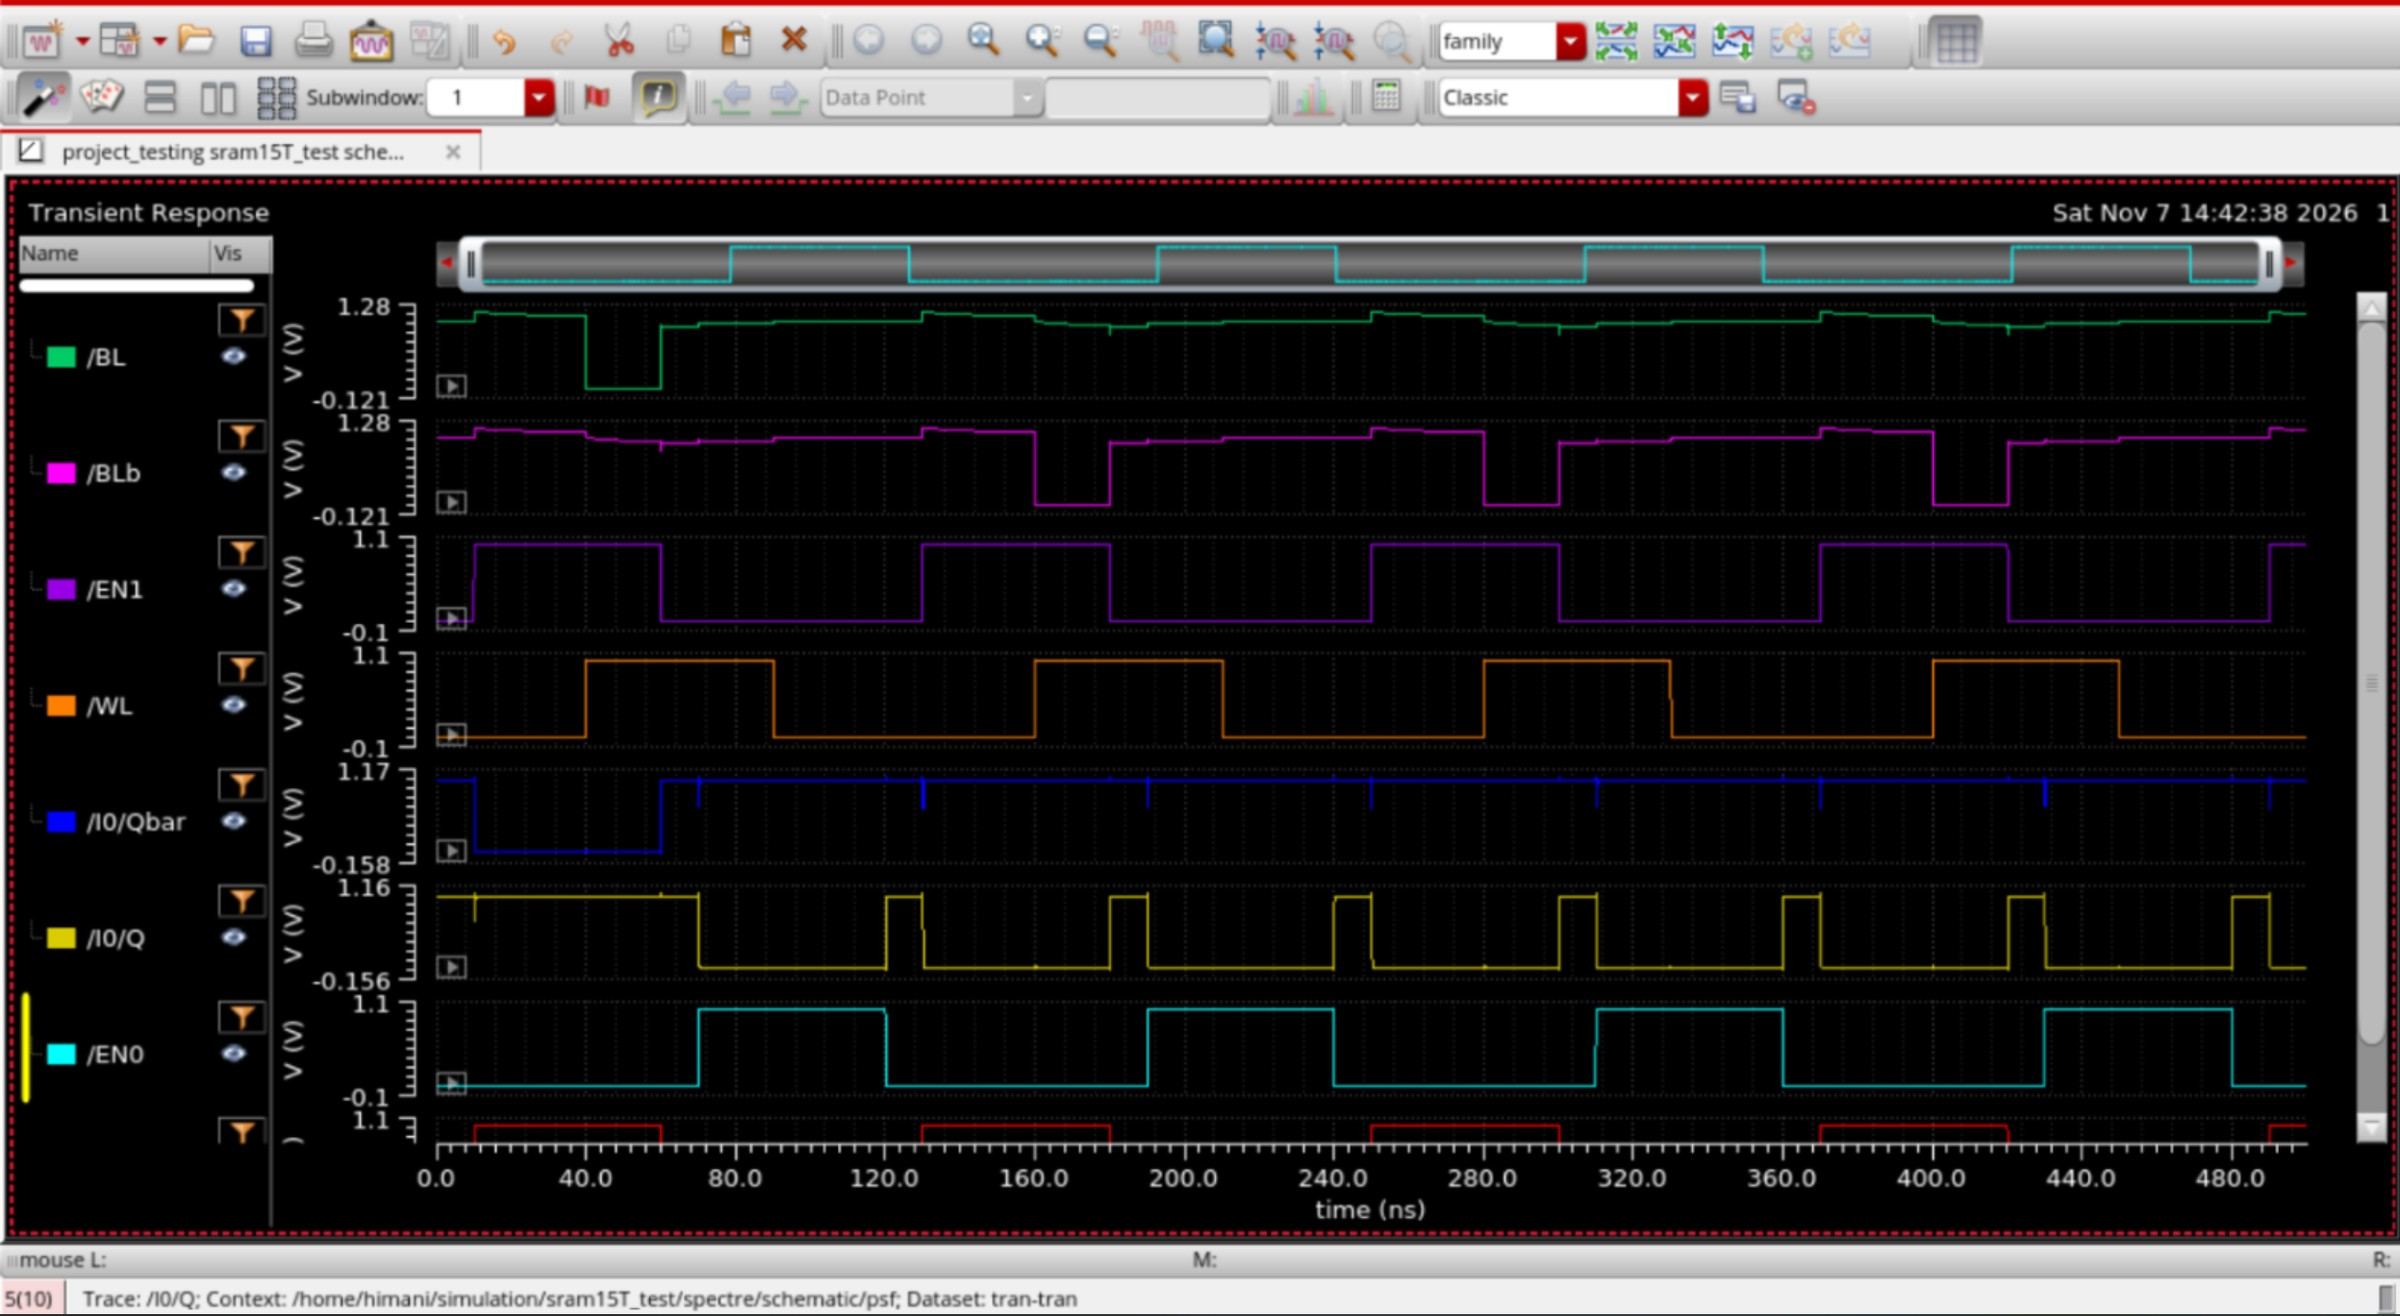
\includegraphics[width=0.90\textwidth]{single_cell_timing_diagram.jpg}
\caption{Single-cell functional transient (Cadence ViVA, 0--500\,ns): \texttt{/BL}, \texttt{/BLb}, \texttt{/EN1}, \texttt{/WL}, \texttt{/I0/Qbar}, \texttt{/I0/Q}, \texttt{/EN0}.}
\label{fig:viva}
\end{figure*}

\subsection{Single-Cell Timing}
Fig.~\ref{fig:viva} shows a single-cell run over 0--500\,ns with a 120-ns period. EN1 is high at about 10--60, 130--180, 250--300 and 370--420\,ns, EN0 at 70--120, 190--240, 310--360 and 430--480\,ns, and WL at 40--90, 160--210, 280--330 and 400--450\,ns. Before 10\,ns both enables are low and Q and Qbar are precharged high. When EN1 rises the latch resolves, with Qbar falling and Q staying high. With WL and EN1 both high (40--60\,ns) \texttt{/BL} discharges. When EN1 falls Qbar is precharged again, and when EN0 rises the cell re-evaluates through the other pull-down pair and Q falls. In later cycles \texttt{/BLb} discharges during the WL--EN1 overlap instead (160--180, 280--300 and 400--420\,ns).

\subsection{Monte Carlo Testbench}
Monte Carlo simulation with local mismatch was run on the 16$\times$16 array (256 cells) and on a 32$\times$64 array (2048 cells). Each run is a 0--125\,ns transient containing two evaluations. The bit is the mean \texttt{/BL} voltage inside a 6-ns window compared with $\VDD/2$\,=\,0.45\,V; the windows are 37--43\,ns for Mode~2 and 97--103\,ns for Mode~1. BLb was exported as a check. Table~\ref{tab:runs} lists the runs.

\begin{table}[!t]
\caption{Monte Carlo Runs}
\label{tab:runs}
\centering
\footnotesize
\begin{tabular}{@{}>{\raggedright\arraybackslash}p{0.27\columnwidth}>{\raggedright\arraybackslash}p{0.50\columnwidth}r@{}}
\toprule
Sweep & Conditions & Cells \\
\midrule
Supply/tilt, 27\,$^\circ$C & $\VDD$\,=\,0.8, 0.9, 1.0\,V; $\Vd$\,=\,0, $\pm$50, $\pm$80, $\pm$120\,mV & 16$\times$16 \\
Temperature, 0.9\,V & $-100$, $-40$, 0, 27, 75\,$^\circ$C; same tilts & 16$\times$16 \\
Large array, 27\,$^\circ$C & 0.9\,V; 0 and $\pm$120\,mV & 32$\times$64 \\
\bottomrule
\end{tabular}
\end{table}

\subsection{Metrics}
The golden key is the response at 27\,$^\circ$C, 0.9\,V and zero tilt. Following \cite{chen2024},
\begin{equation}
\mathrm{BER}=\frac{1}{m}\sum_{i=1}^{m}\frac{\mathrm{HD}\left(R,R_i\right)}{n}\times100\%,
\end{equation}
with $R$ the golden key, $R_i$ the response under condition $i$ and $n$ bits; here $m=2$ (the $+$ and $-$ tilt). ``Unstable bits'' is the fraction of cells whose $+$tilt and $-$tilt responses differ. For an $N$-bit key, assuming independent errors,
\begin{equation}
\mathrm{BLER}_N = 1-(1-\mathrm{BER})^{N},\qquad N\in\{128,256\}.
\end{equation}
A condition used to choose the healing or a mask is in sample: its residual BER is zero by construction and is marked as such.

\subsection{Cadence Server Locations}
Table~\ref{tab:paths} and Fig.~\ref{fig:tree} give the server locations of the design and simulation data. The ViVA window of the single-cell run identifies library \texttt{project\_testing}, cell \texttt{sram15T\_test}, view \texttt{schematic}; the array is cell \texttt{16x16array} in library \texttt{project}.

\begin{table}[!t]
\caption{Server Locations}
\label{tab:paths}
\centering
\footnotesize
\begin{tabular}{@{}>{\raggedright\arraybackslash}p{0.30\columnwidth}>{\raggedright\arraybackslash}p{0.62\columnwidth}@{}}
\toprule
Purpose & Path \\
\midrule
All circuits used in the project & \path{/home/himani/Work/UMC28_test/cds/project/} \\
All testing done on the SRAM cell & \path{/home/himani/Work/UMC28_test/cds/project_testing/sram15T_test/} \\
All CSVs generated for the MC simulations & \path{/home/himani/simulation/project_testing/sram15T_test/} \\
Single-cell transient results (ViVA) & \path{/home/himani/simulation/sram15T_test/spectre/schematic/psf} (dataset \texttt{tran-tran}) \\
\bottomrule
\end{tabular}
\end{table}

\begin{figure}[!t]
\centering
\begin{minipage}{\columnwidth}
\begin{Verbatim}[fontsize=\scriptsize,frame=single]
/home/himani/
|-- Work/UMC28_test/cds/
|   |-- project/          (all project circuits)
|   `-- project_testing/
|       `-- sram15T_test/ (SRAM cell testbench)
`-- simulation/
    |-- project_testing/
    |   `-- sram15T_test/ (MC CSV exports)
    `-- sram15T_test/spectre/schematic/psf/
                          (single-cell tran-tran)
\end{Verbatim}
\end{minipage}
\caption{Server directory tree for design and simulation data.}
\label{fig:tree}
\end{figure}

% ===================== result wide floats =====================
\begin{figure*}[!t]
\centering
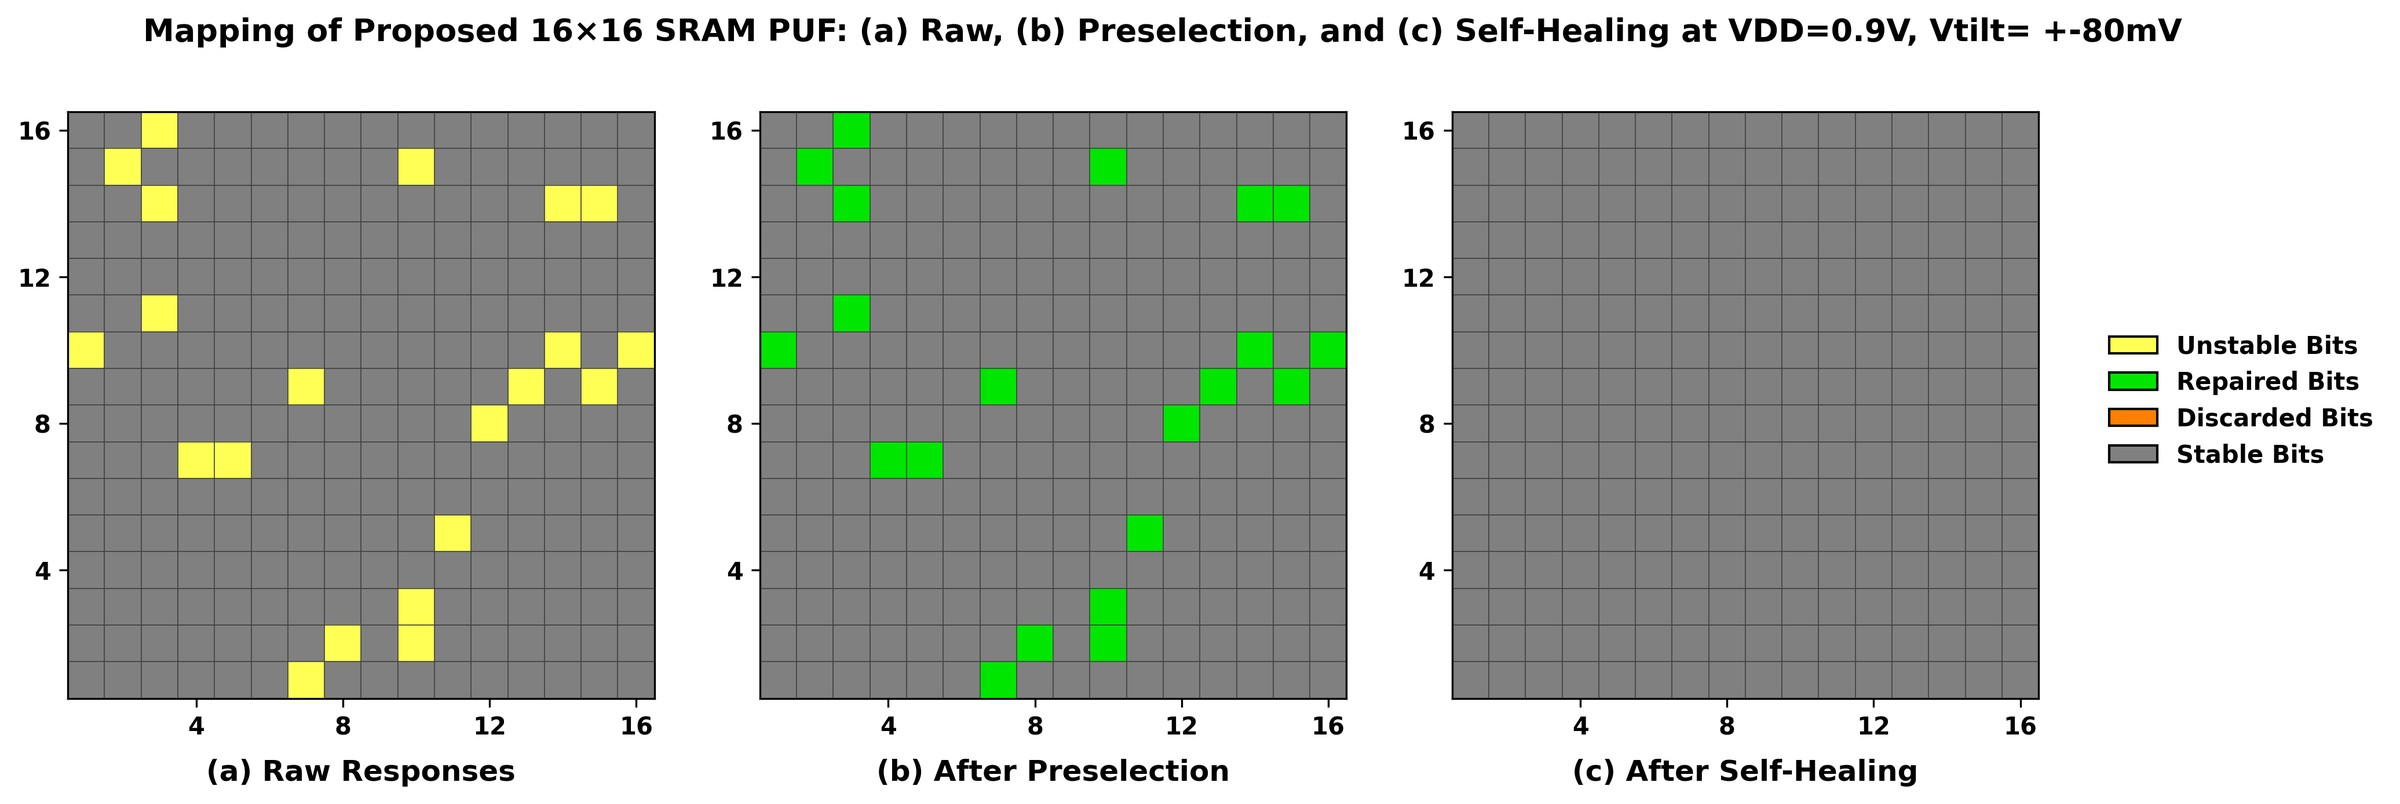
\includegraphics[width=0.49\textwidth]{nb18_map16_27C_VDD0.9_tilt80.jpg}\hfill
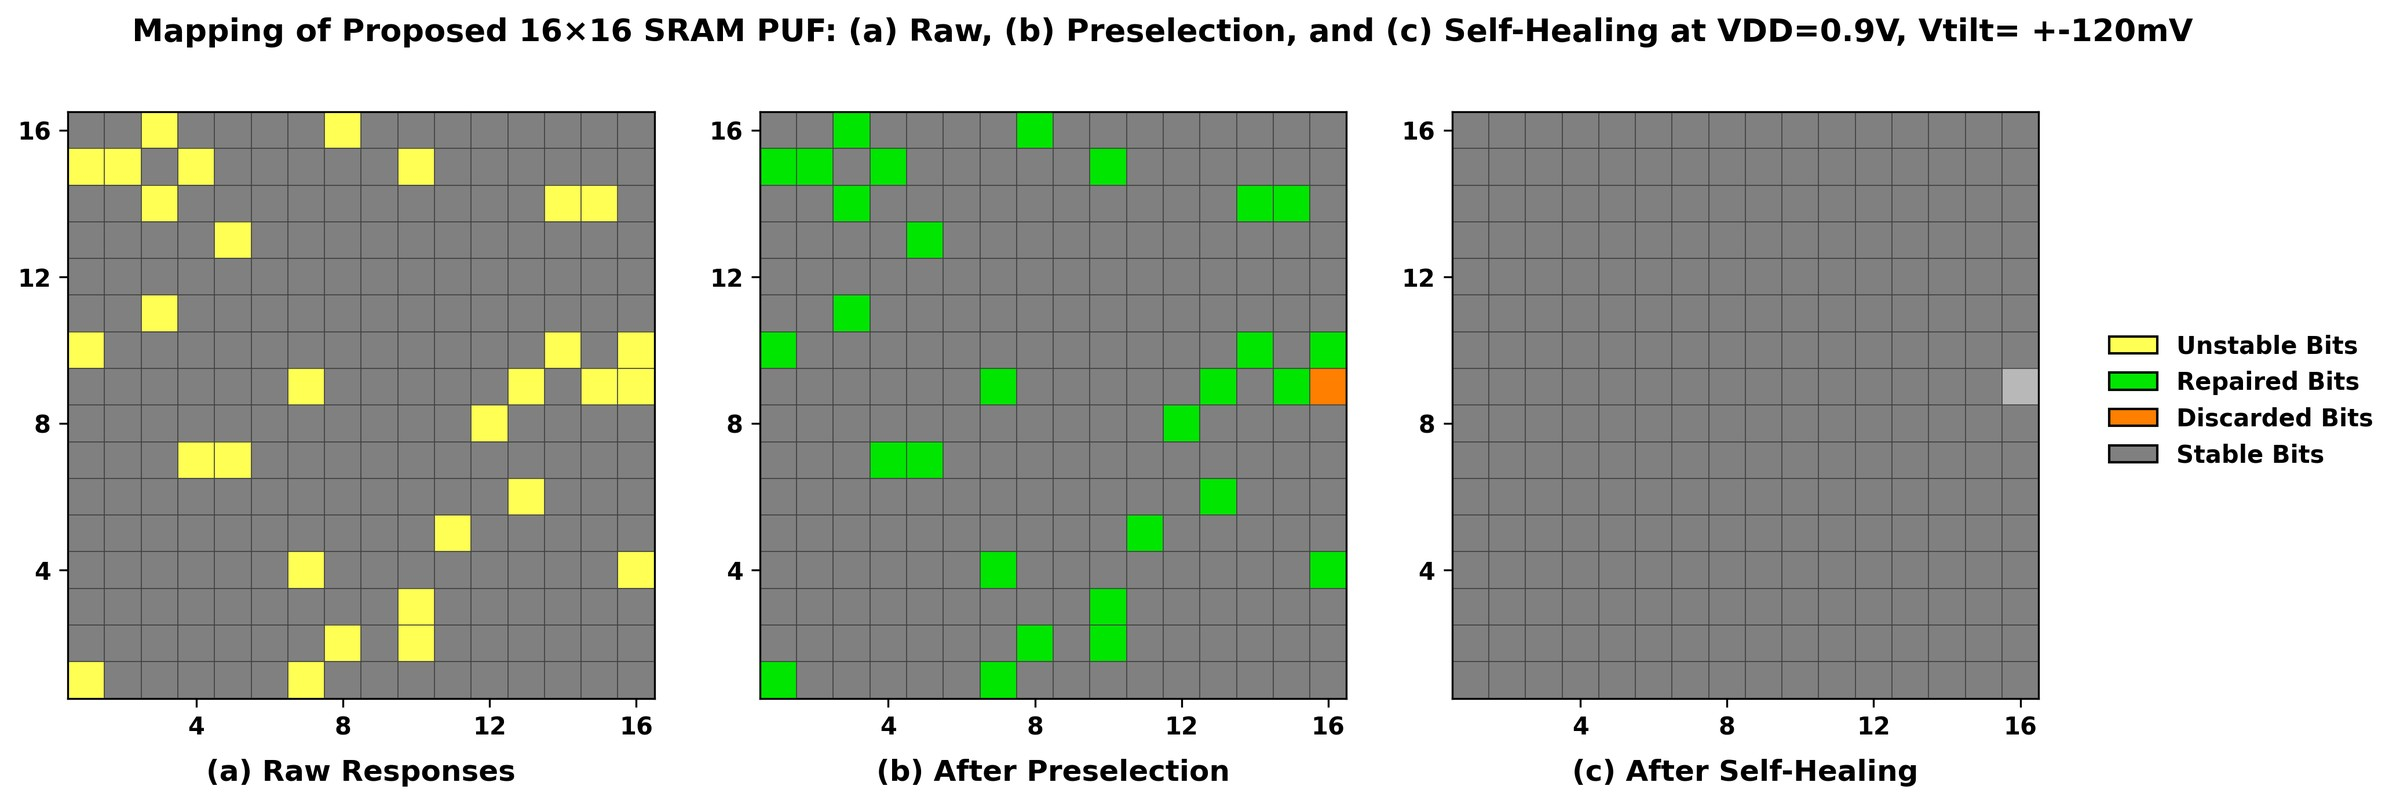
\includegraphics[width=0.49\textwidth]{nb20_map16_27C_VDD0.9_tilt120.jpg}\\[2pt]
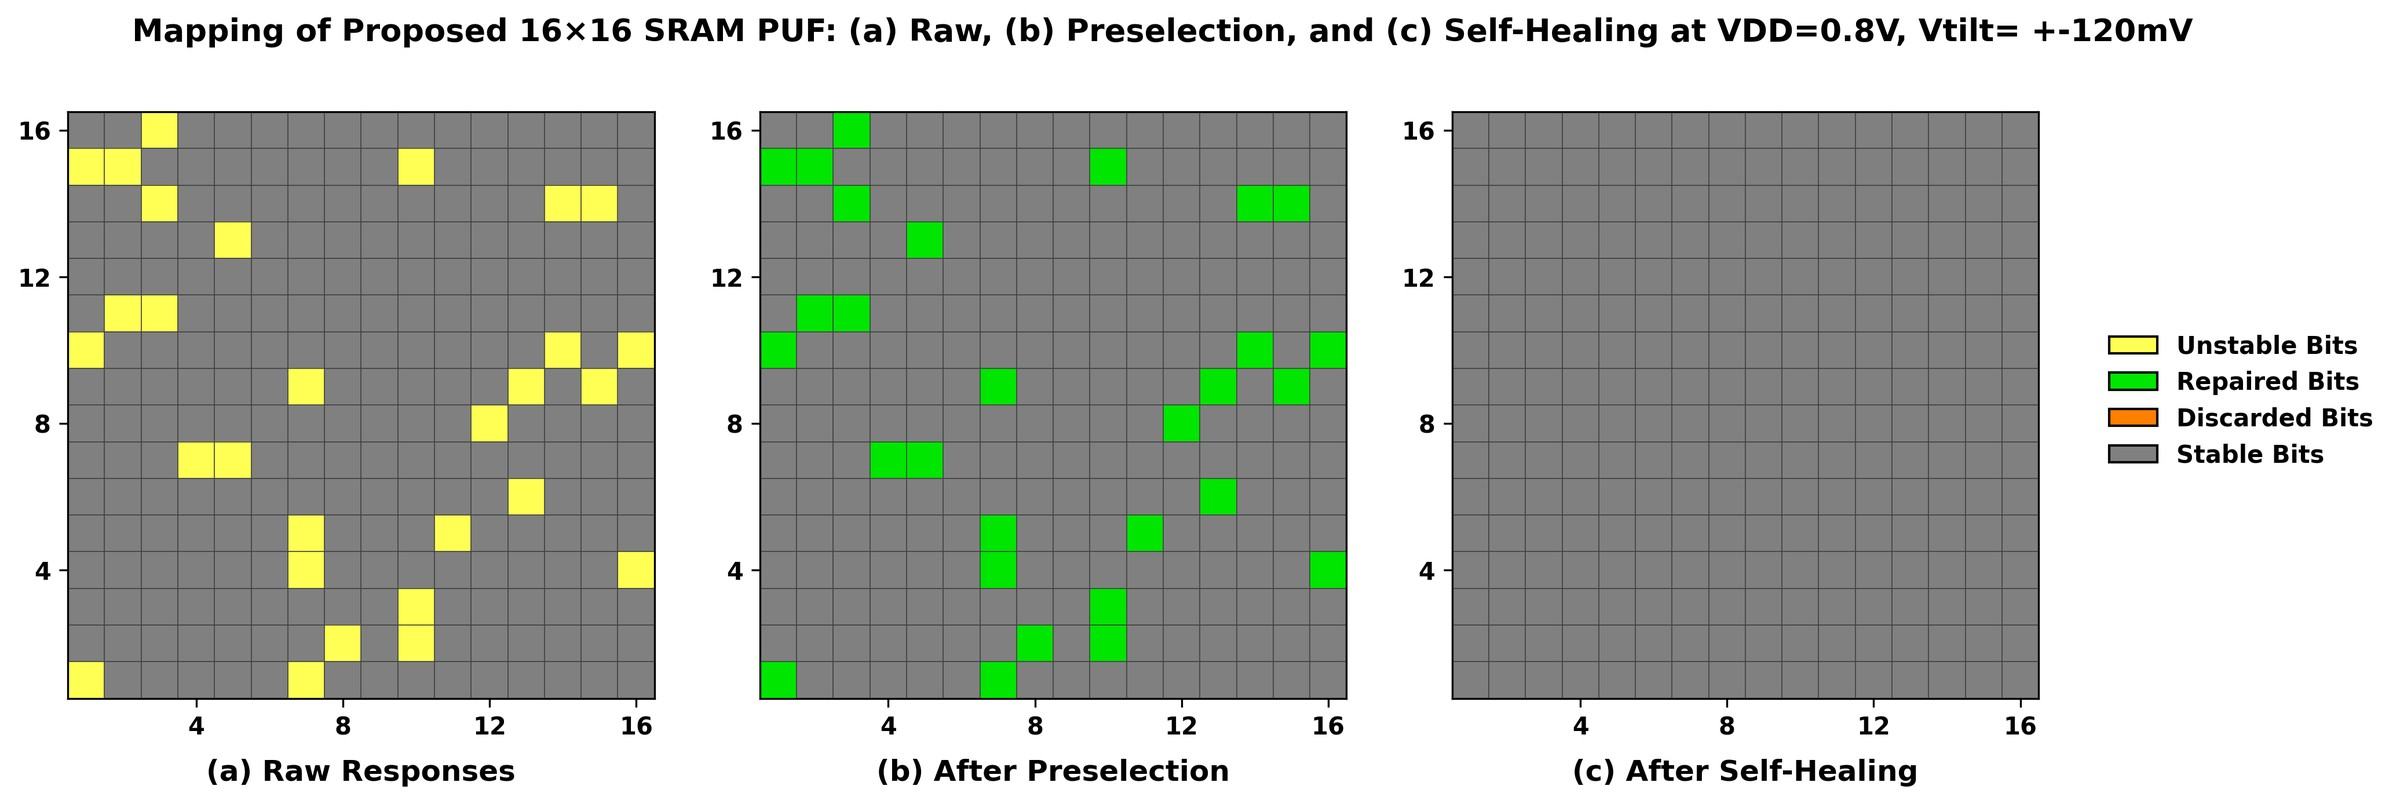
\includegraphics[width=0.49\textwidth]{nb29_map16_27C_VDD0.8_tilt120.jpg}\hfill
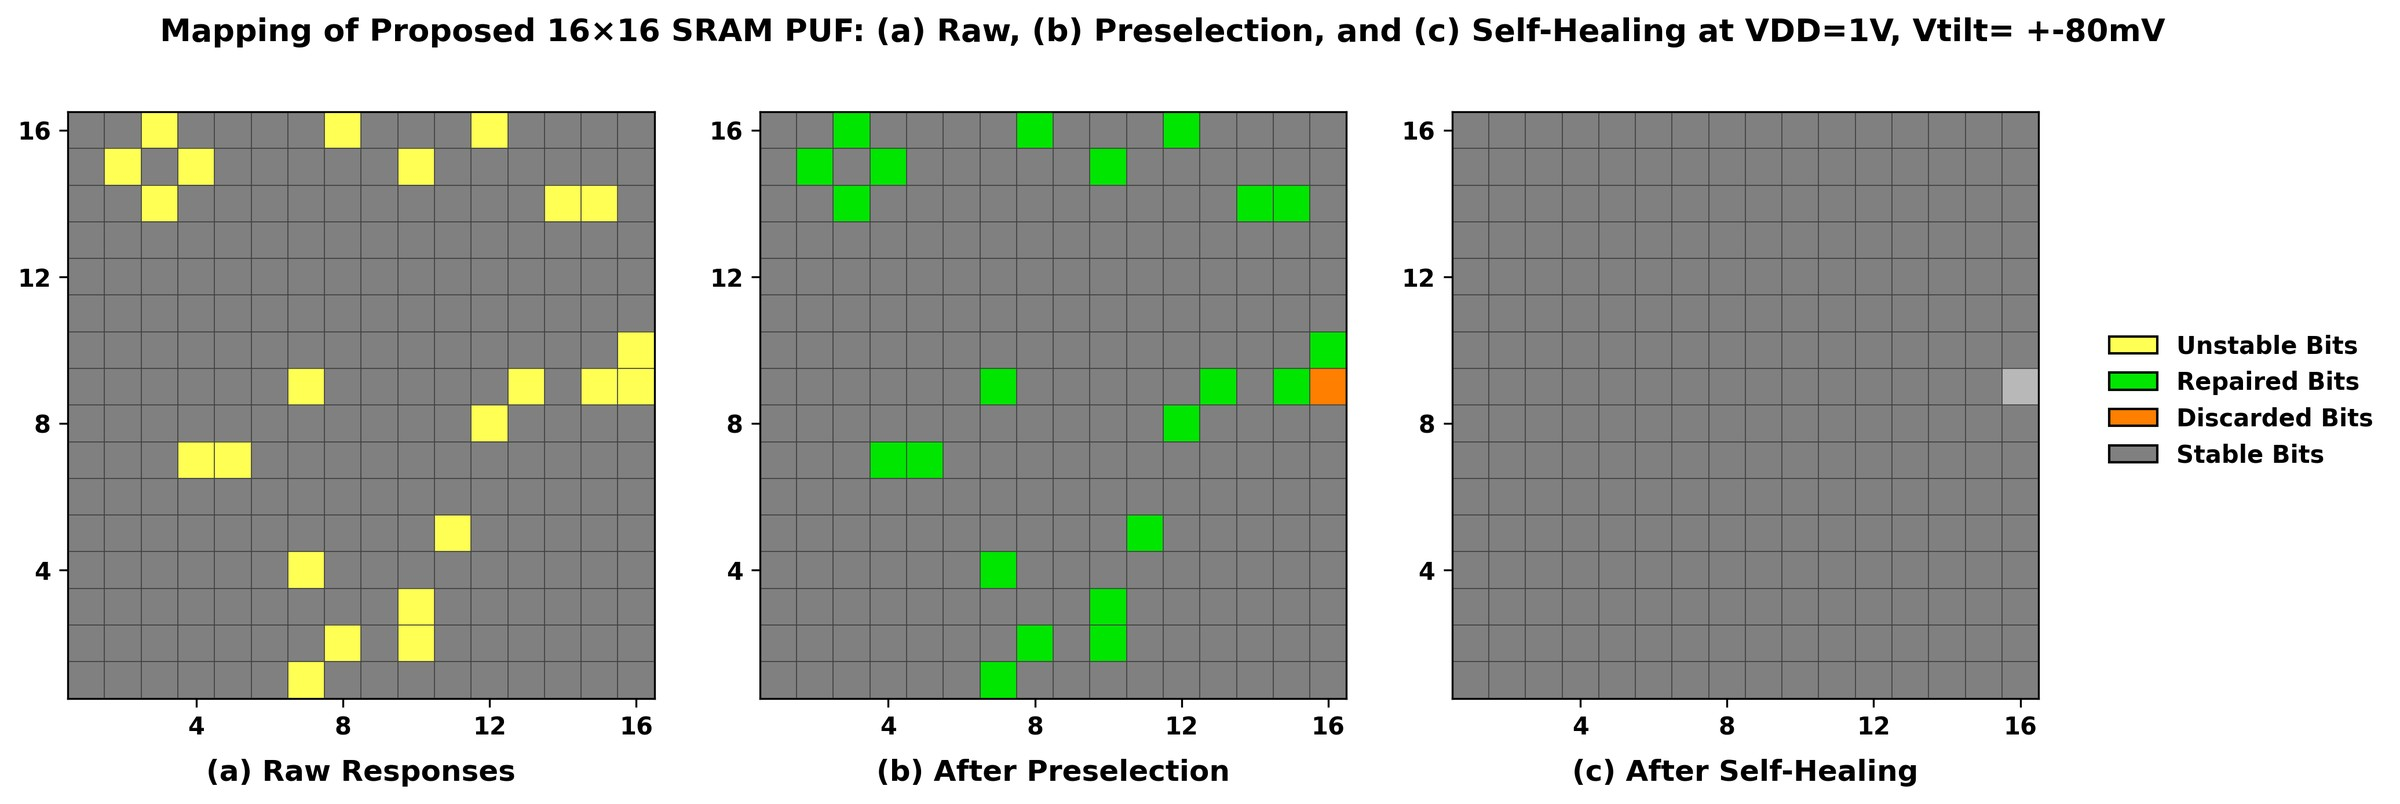
\includegraphics[width=0.49\textwidth]{nb21_map16_27C_VDD1.0_tilt80.jpg}\\[2pt]
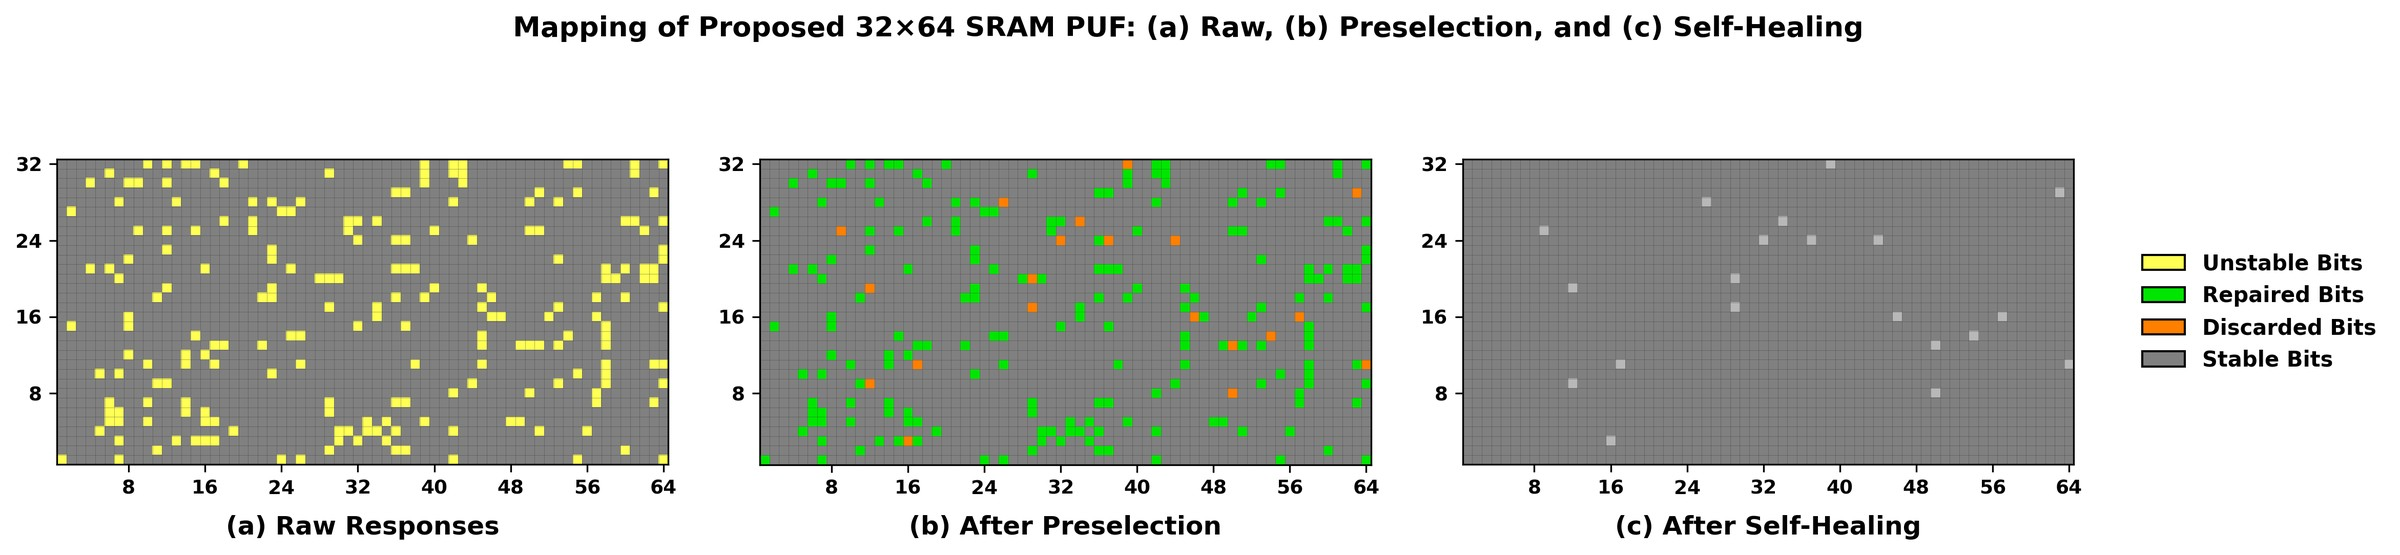
\includegraphics[width=0.72\textwidth]{nb30_map32x64_27C_VDD0.9_tilt120.jpg}
\caption{Bit-classification maps at 27\,$^\circ$C: (a) raw, (b) after preselection, (c) after self-healing. Top: 16$\times$16 array at $\VDD=0.9$\,V, $\pm80$\,mV (left) and $\pm120$\,mV (right). Middle: 0.8\,V, $\pm120$\,mV (left); 1.0\,V, $\pm80$\,mV (right). Bottom: 32$\times$64 array, 0.9\,V, $\pm120$\,mV. Grey: stable; yellow: unstable; green: repaired (Mode~2); orange: discarded.}
\label{fig:maps}
\end{figure*}

\begin{figure*}[!t]
\centering
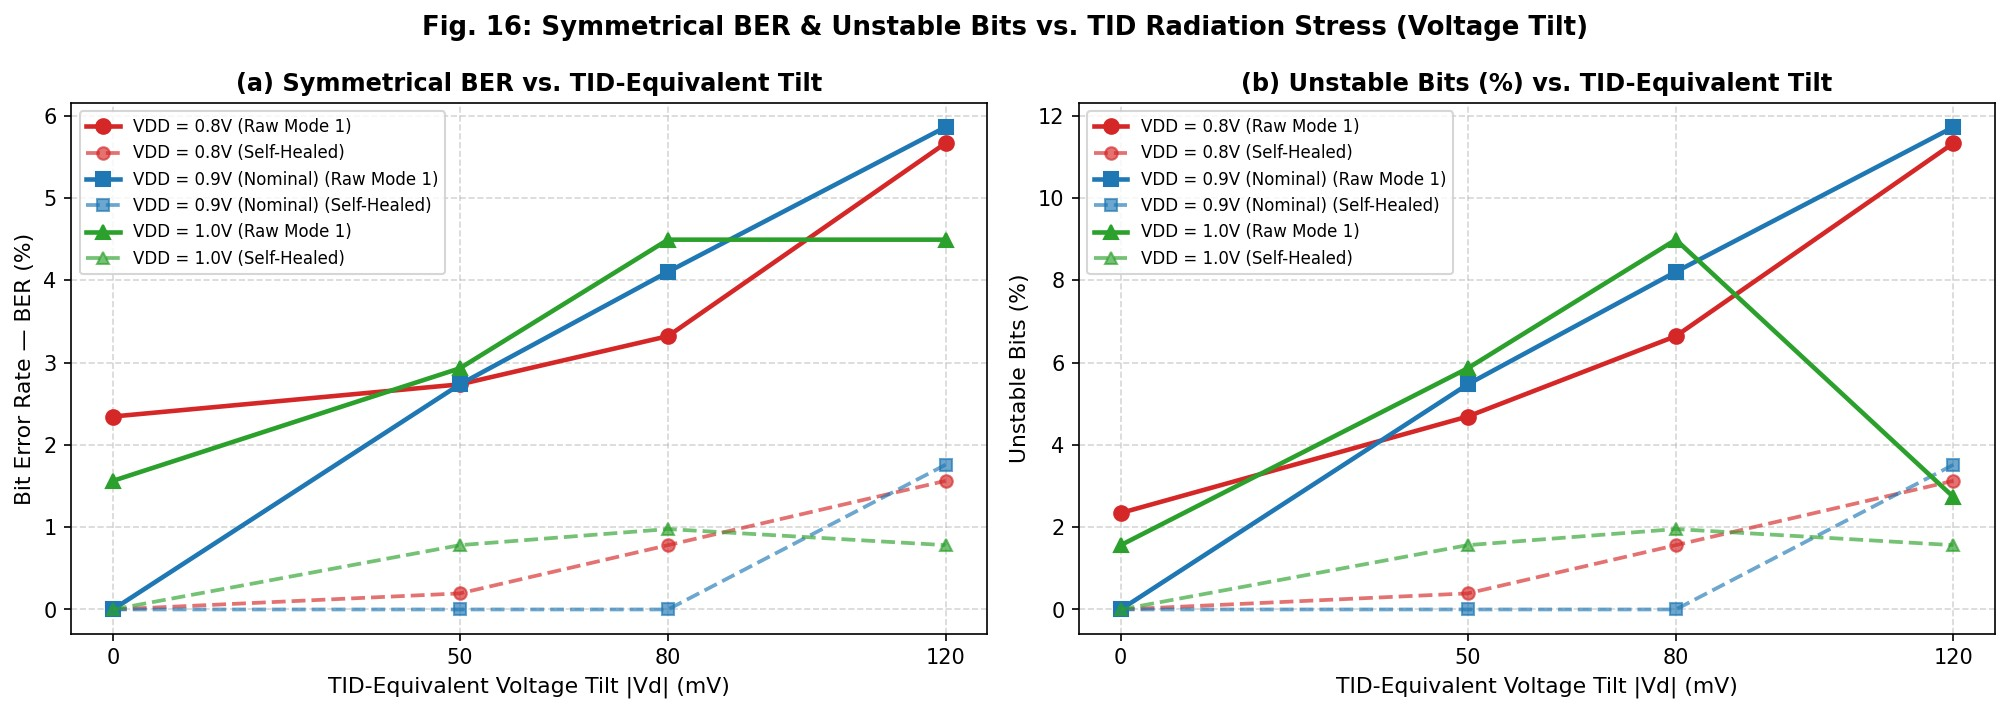
\includegraphics[width=0.70\textwidth]{nb31_ber_unstable_vs_tilt.jpg}\\[2pt]
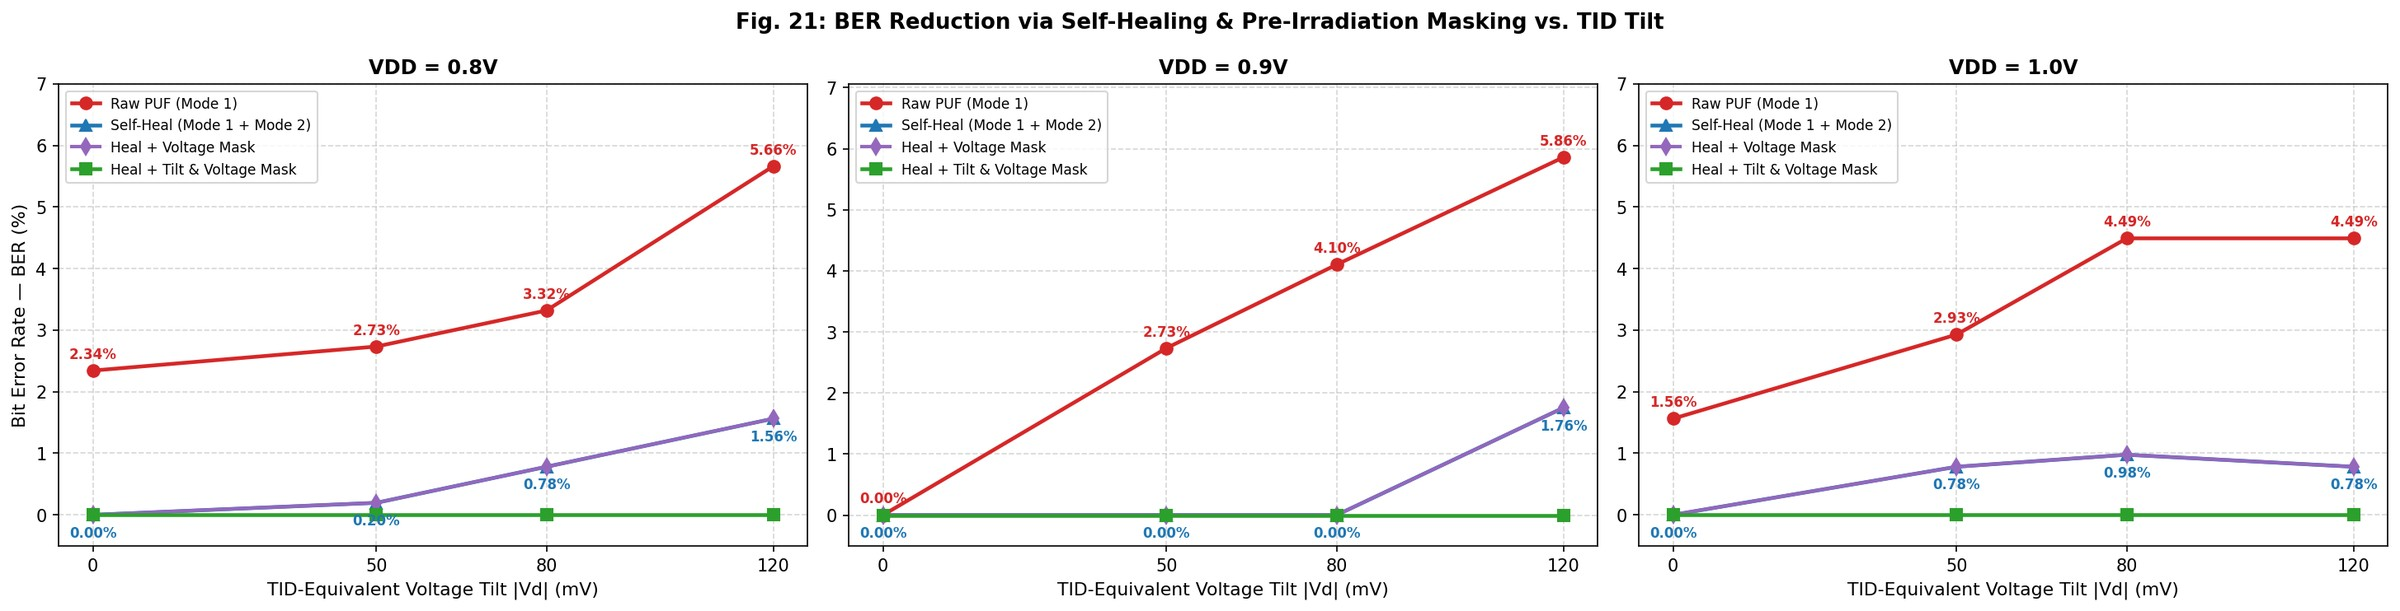
\includegraphics[width=0.78\textwidth]{nb31_ber_selfheal_masking_vs_tilt.jpg}
\caption{Top: (a) BER against the golden key and (b) unstable bits against tilt magnitude, raw Mode~1 (solid) and self-healed (dashed). Bottom: raw, self-healed, healed with voltage mask, and healed with tilt-and-voltage mask, per supply. Healing chosen at 0.9\,V, $\pm80$\,mV.}
\label{fig:bertilt}
\end{figure*}

\section{Monte Carlo Results}
\subsection{Logic Balance}
In every run BLb was the exact complement of BL, so every cell resolved fully in both windows. The tilt acts in one direction: at 0.9\,V the number of Mode~1 ones is 150, 147, 139, 133 and 129 of 256 for $-80$, $-50$, 0, $+50$ and $+80$\,mV, and 1205 and 994 of 2048 at $-120$ and $+120$\,mV. A negative tilt (VDDL\,$<$\,VDDR) adds ones and a positive tilt removes them, as the trip-point argument predicts.

\subsection{Preselection and Self-Healing at 27\,$^\circ$C}
Table~\ref{tab:presel} and Fig.~\ref{fig:maps} summarise preselection. At 0.8 and 0.9\,V the unstable fraction rises with $|\Vd|$ because more cells have a mismatch smaller than the tilt: 5.47, 8.20 and 11.72\% at 0.9\,V for 50, 80 and 120\,mV. Mode~2 repairs 93--100\% of these cells, and at most one of 256 is discarded. In the 32$\times$64 array at $\pm120$\,mV, 211 cells (10.30\%) are unstable, 191 are repaired and 20 discarded, a valid yield of 99.02\%. Mode~2 is unstable in 227 cells (11.08\%), so independent modes would leave $2048\times0.103\times0.111\approx23$ cells unstable in both; 20 were observed. Unstable cells are scattered with no row or column pattern, as expected for independent mismatch.

\begin{table}[!t]
\caption{Preselection Outcome at 27\,$^\circ$C}
\label{tab:presel}
\centering
\footnotesize
\setlength{\tabcolsep}{3.4pt}
\begin{tabular}{@{}ccrrrrr@{}}
\toprule
$\VDD$ (V) & $|\Vd|$ (mV) & Unstable & Rep. & Disc. & Heal eff. & Yield \\
\midrule
0.8 & 50 & 12 (4.69\%) & 12 & 0 & 100\% & 100\% \\
0.8 & 80 & 17 (6.64\%) & 17 & 0 & 100\% & 100\% \\
0.8 & 120 & 29 (11.33\%) & 29 & 0 & 100\% & 100\% \\
0.9 & 50 & 14 (5.47\%) & 14 & 0 & 100\% & 100\% \\
0.9 & 80 & 21 (8.20\%) & 21 & 0 & 100\% & 100\% \\
0.9 & 120 & 30 (11.72\%) & 29 & 1 & 96.67\% & 99.61\% \\
1.0 & 50 & 15 (5.86\%) & 14 & 1 & 93.33\% & 99.61\% \\
1.0 & 80 & 23 (8.98\%) & 22 & 1 & 95.65\% & 99.61\% \\
1.0 & 120 & 19 (7.42\%) & 19 & 0 & 100\% & 100\% \\
\midrule
0.9$^\dagger$ & 120 & 211 (10.30\%) & 191 & 20 & 90.52\% & 99.02\% \\
\bottomrule
\multicolumn{7}{@{}l}{\scriptsize 16$\times$16 array (256 cells); $^\dagger$32$\times$64 array (2048 cells).}
\end{tabular}
\end{table}

\subsection{Golden Keys and Uniformity}
The Mode~1 and Mode~2 golden keys of the 16$\times$16 array (hexadecimal) are \texttt{6CD4700E\ldots E5A732} and \texttt{75476AB7\ldots 735345}, with 139 (54.3\%) and 146 (57.0\%) ones; full keys are in \path{results/golden_keys_27C_0.9V.csv}. They differ in 125 of 256 positions (48.8\%), close to the 50\% expected for independent responses. The healed 2028-bit key of the 32$\times$64 array has 54.49\% ones, about four binomial standard deviations above 50\%, so the bias toward 1 is systematic; cell asymmetry, unequal BL/BLb loading or the $\VDD/2$ decision threshold are possible causes.

\subsection{BER Against Supply and Tilt}
Table~\ref{tab:ber} and Figs.~\ref{fig:bertilt} and \ref{fig:bervdd} give BER against the golden key, with healing chosen at 0.9\,V, $\pm80$\,mV. Raw Mode~1 BER reaches 5.86\% at $\pm120$\,mV, and 2.34\% and 1.56\% at 0.8 and 1.0\,V with no tilt. Outside the healing condition, self-healing lowers BER by 3--4$\times$: 5.86\% to 1.76\% at 0.9\,V, $\pm120$\,mV, and 5.66\% to 1.56\% at 0.8\,V, $\pm120$\,mV. With no tilt the healed key has zero errors at all three supplies. At 0.9\,V the unstable fraction is exactly twice the BER, because an unstable cell matches the golden key in one tilt direction and not the other. The voltage mask, built from the zero-tilt runs at 0.8 and 1.0\,V, removes no further errors because the healed key already has none there; the tilt-and-voltage mask gives 0\% because it is evaluated on the runs it was built from.

\begin{table}[!t]
\caption{BER (\%) Against the Golden Key, 27\,$^\circ$C, Mean of $\pm$Tilt}
\label{tab:ber}
\centering
\footnotesize
\setlength{\tabcolsep}{3.6pt}
\begin{tabular}{@{}ccrrrrr@{}}
\toprule
$\VDD$ (V) & $|\Vd|$ (mV) & Raw M1 & Raw M2 & Healed & Unst. M1 & Unst. heal. \\
\midrule
0.8 & 0 & 2.34 & 1.95 & 0.00 & 2.34 & 0.00 \\
0.8 & 50 & 2.73 & 1.95 & 0.20 & 4.69 & 0.39 \\
0.8 & 80 & 3.32 & 3.32 & 0.78 & 6.64 & 1.56 \\
0.8 & 120 & 5.66 & 4.10 & 1.56 & 11.33 & 3.13 \\
0.9 & 50 & 2.73 & 2.15 & 0.00 & 5.47 & 0.00 \\
0.9 & 80 & 4.10 & 3.32 & 0.00$^*$ & 8.20 & 0.00 \\
0.9 & 120 & 5.86 & 4.49 & 1.76 & 11.72 & 3.52 \\
1.0 & 0 & 1.56 & 1.56 & 0.00 & 1.56 & 0.00 \\
1.0 & 50 & 2.93 & 1.95 & 0.78 & 5.86 & 1.56 \\
1.0 & 80 & 4.49 & 4.10 & 0.98 & 8.98 & 1.95 \\
1.0 & 120 & 4.49 & 4.30 & 0.78 & 2.73 & 1.56 \\
\bottomrule
\multicolumn{7}{@{}l}{\scriptsize $^*$Condition used to choose the healing (zero by construction).}
\end{tabular}
\end{table}

\begin{figure}[!t]
\centering
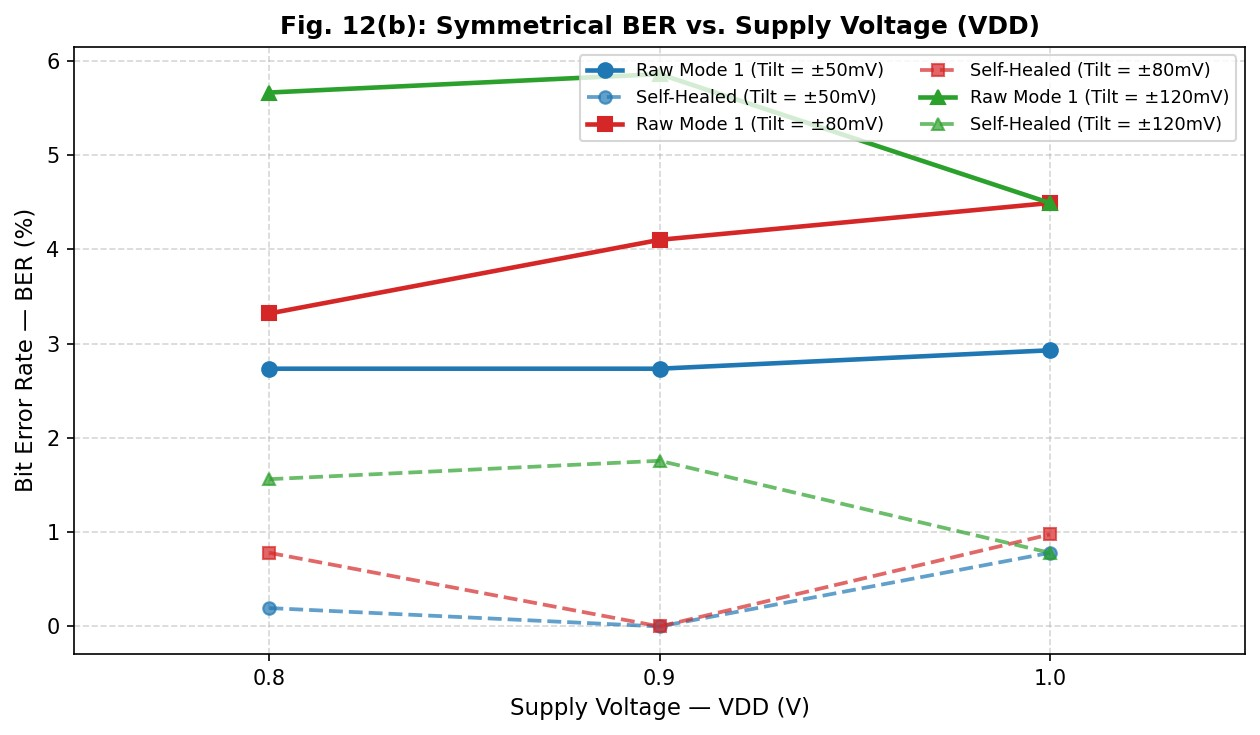
\includegraphics[width=0.95\columnwidth]{nb31_ber_vs_vdd.jpg}
\caption{BER against supply voltage for each tilt, raw Mode~1 (solid) and self-healed (dashed).}
\label{fig:bervdd}
\end{figure}

\begin{figure*}[!t]
\centering
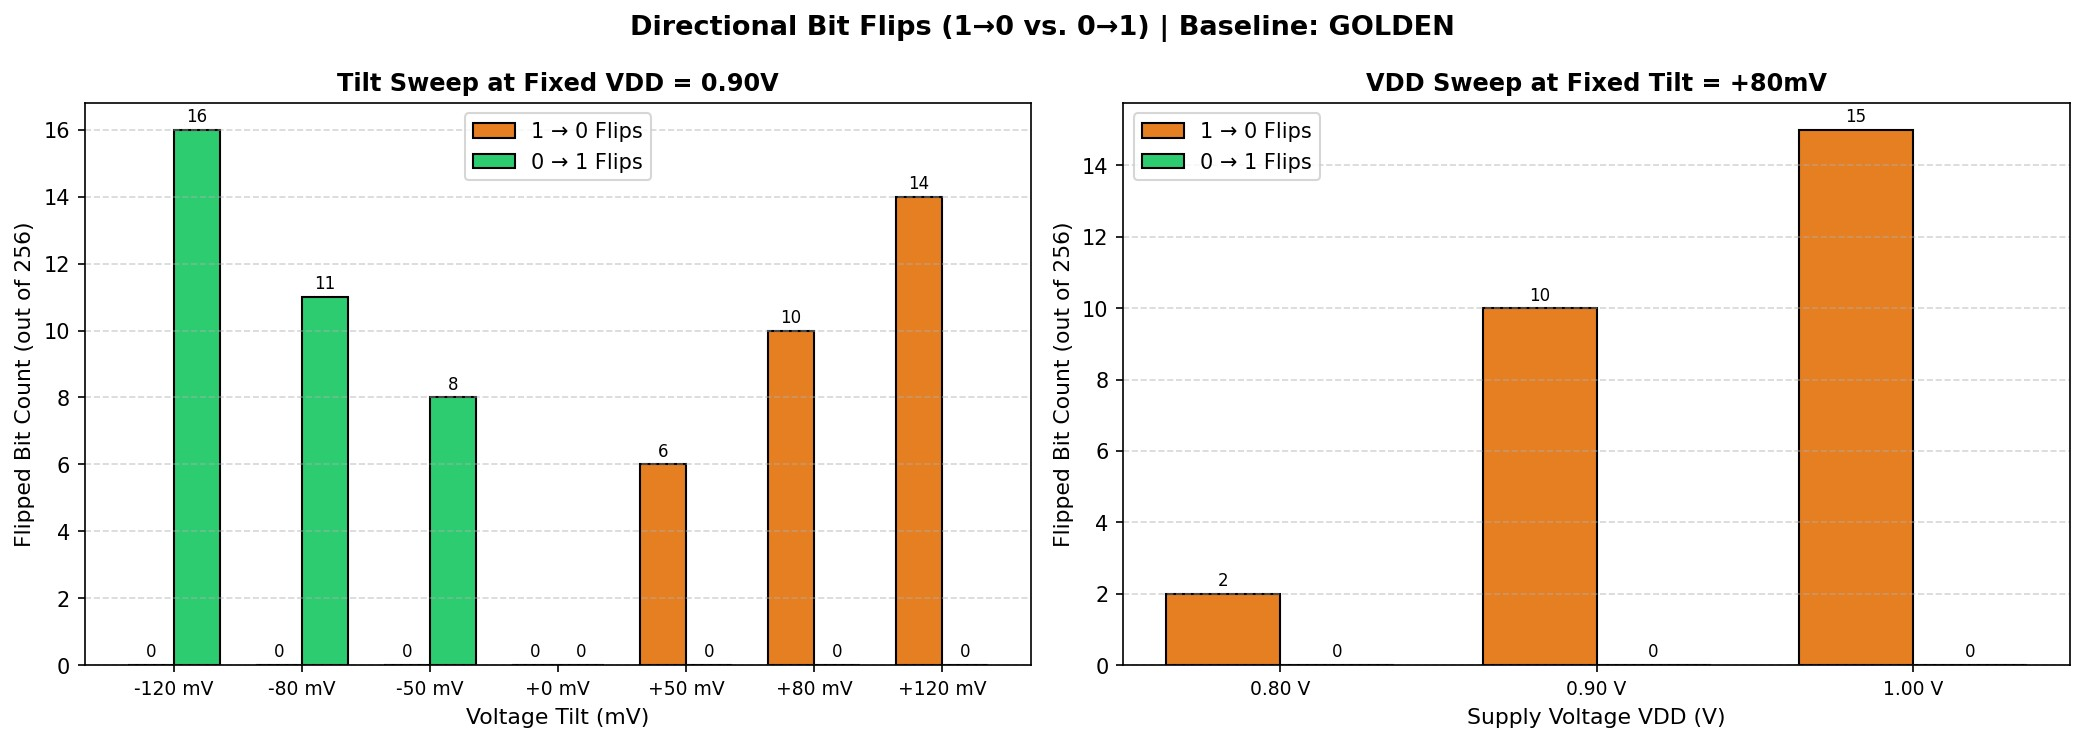
\includegraphics[width=0.75\textwidth]{nb32_directional_flips_tilt_and_vdd_sweeps.jpg}
\caption{Directional bit flips against the golden key (orange: 1$\rightarrow$0; green: 0$\rightarrow$1): tilt sweep at 0.9\,V (left) and supply sweep at $+80$\,mV (right).}
\label{fig:flip}
\end{figure*}

\begin{figure*}[!t]
\centering
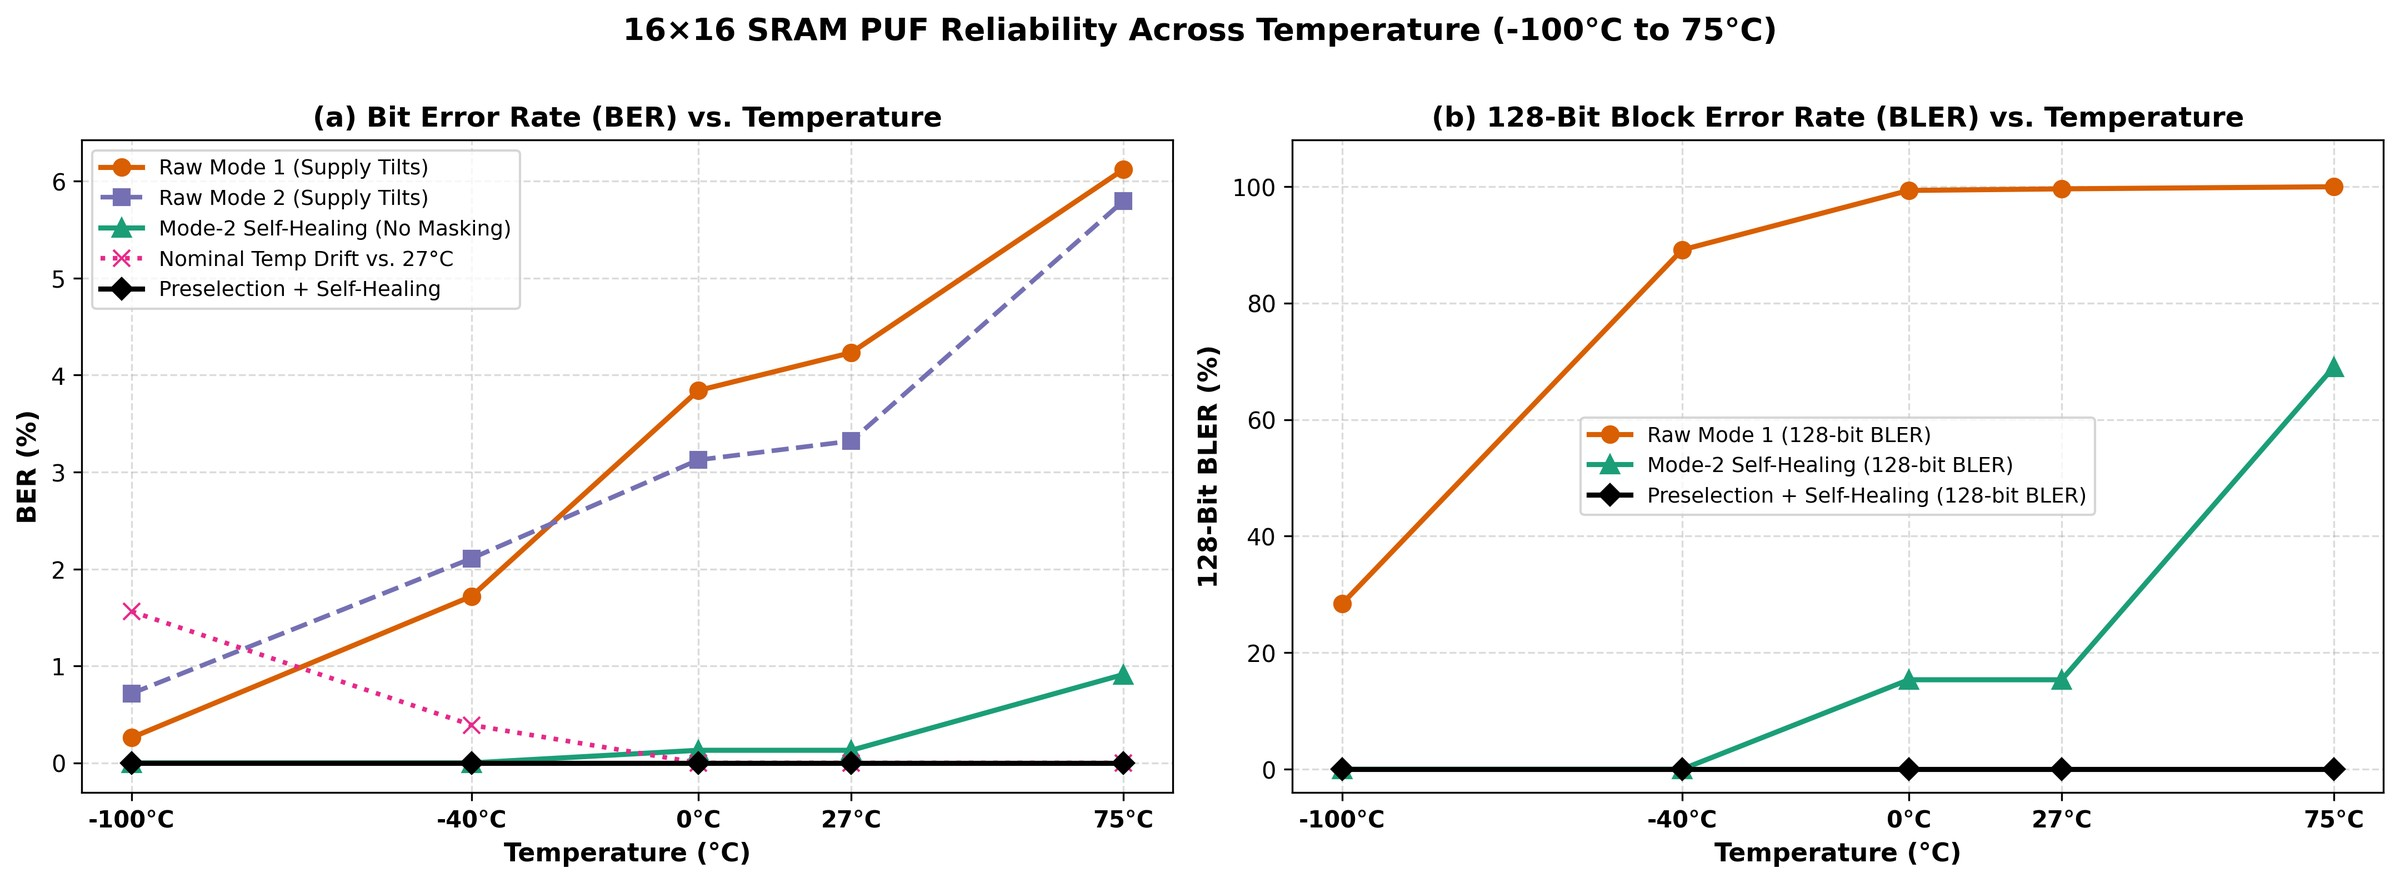
\includegraphics[width=0.72\textwidth]{nb34_ber_bler_vs_temperature.jpg}\\[2pt]
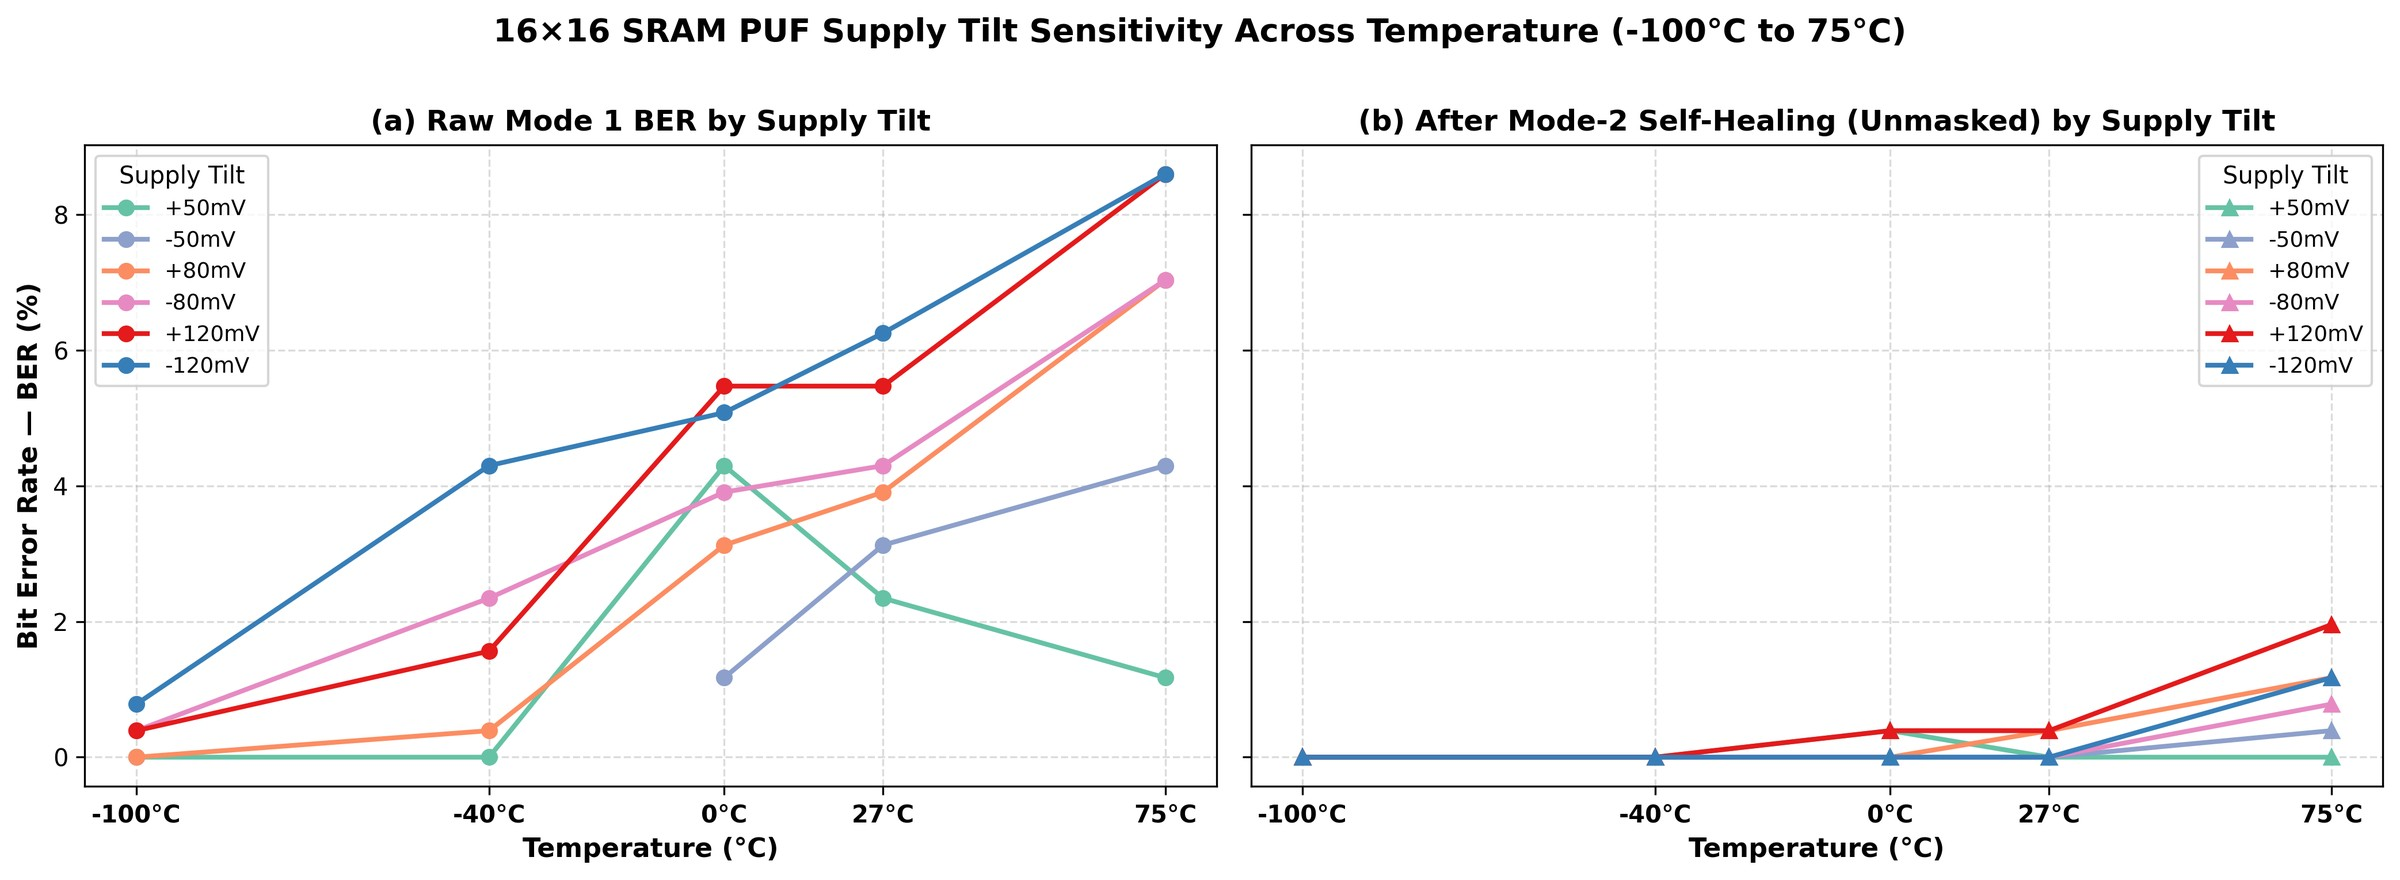
\includegraphics[width=0.72\textwidth]{nb34_tilt_ber_vs_temperature.jpg}
\caption{Temperature sweep at 0.9\,V. Top: (a) mean supply-tilt BER and nominal drift against the 27\,$^\circ$C key, (b) 128- and 256-bit BLER. Bottom: BER for each signed tilt, (a) raw Mode~1 and (b) self-healed (unmasked).}
\label{fig:bertemp}
\end{figure*}

\begin{figure*}[!t]
\centering
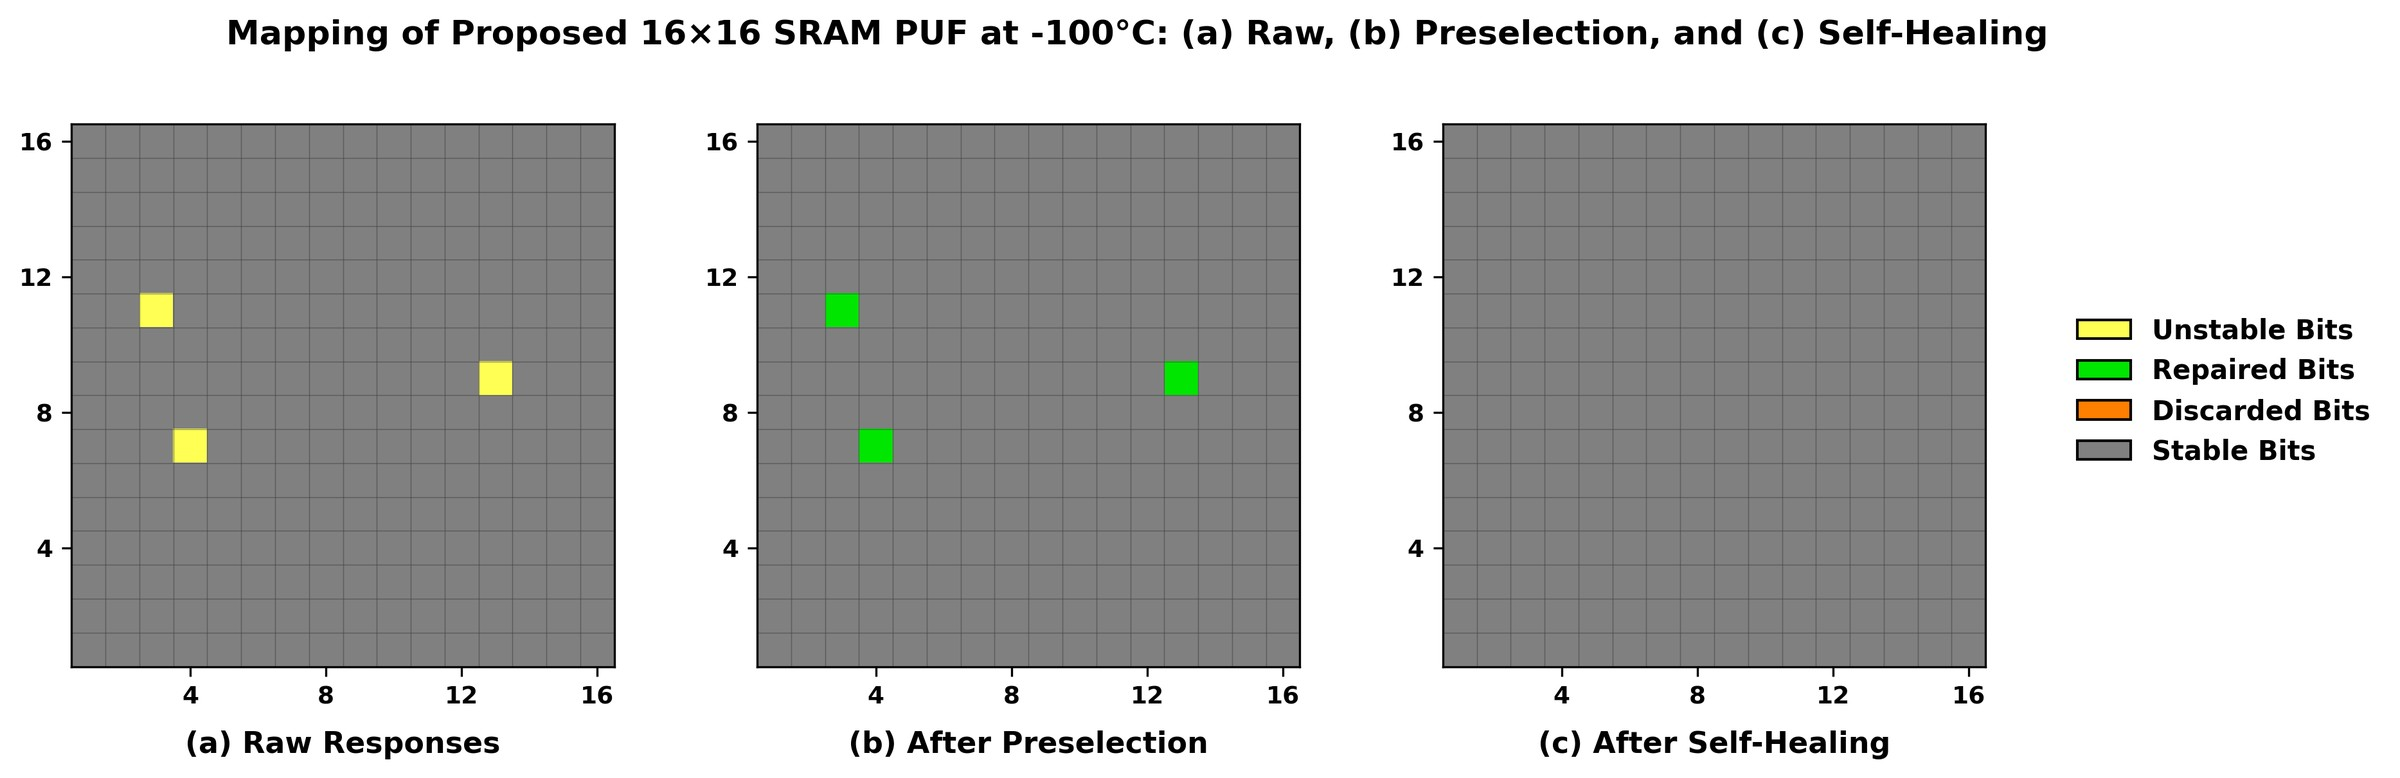
\includegraphics[width=0.49\textwidth]{nb33_map16_T-100C.jpg}\hfill
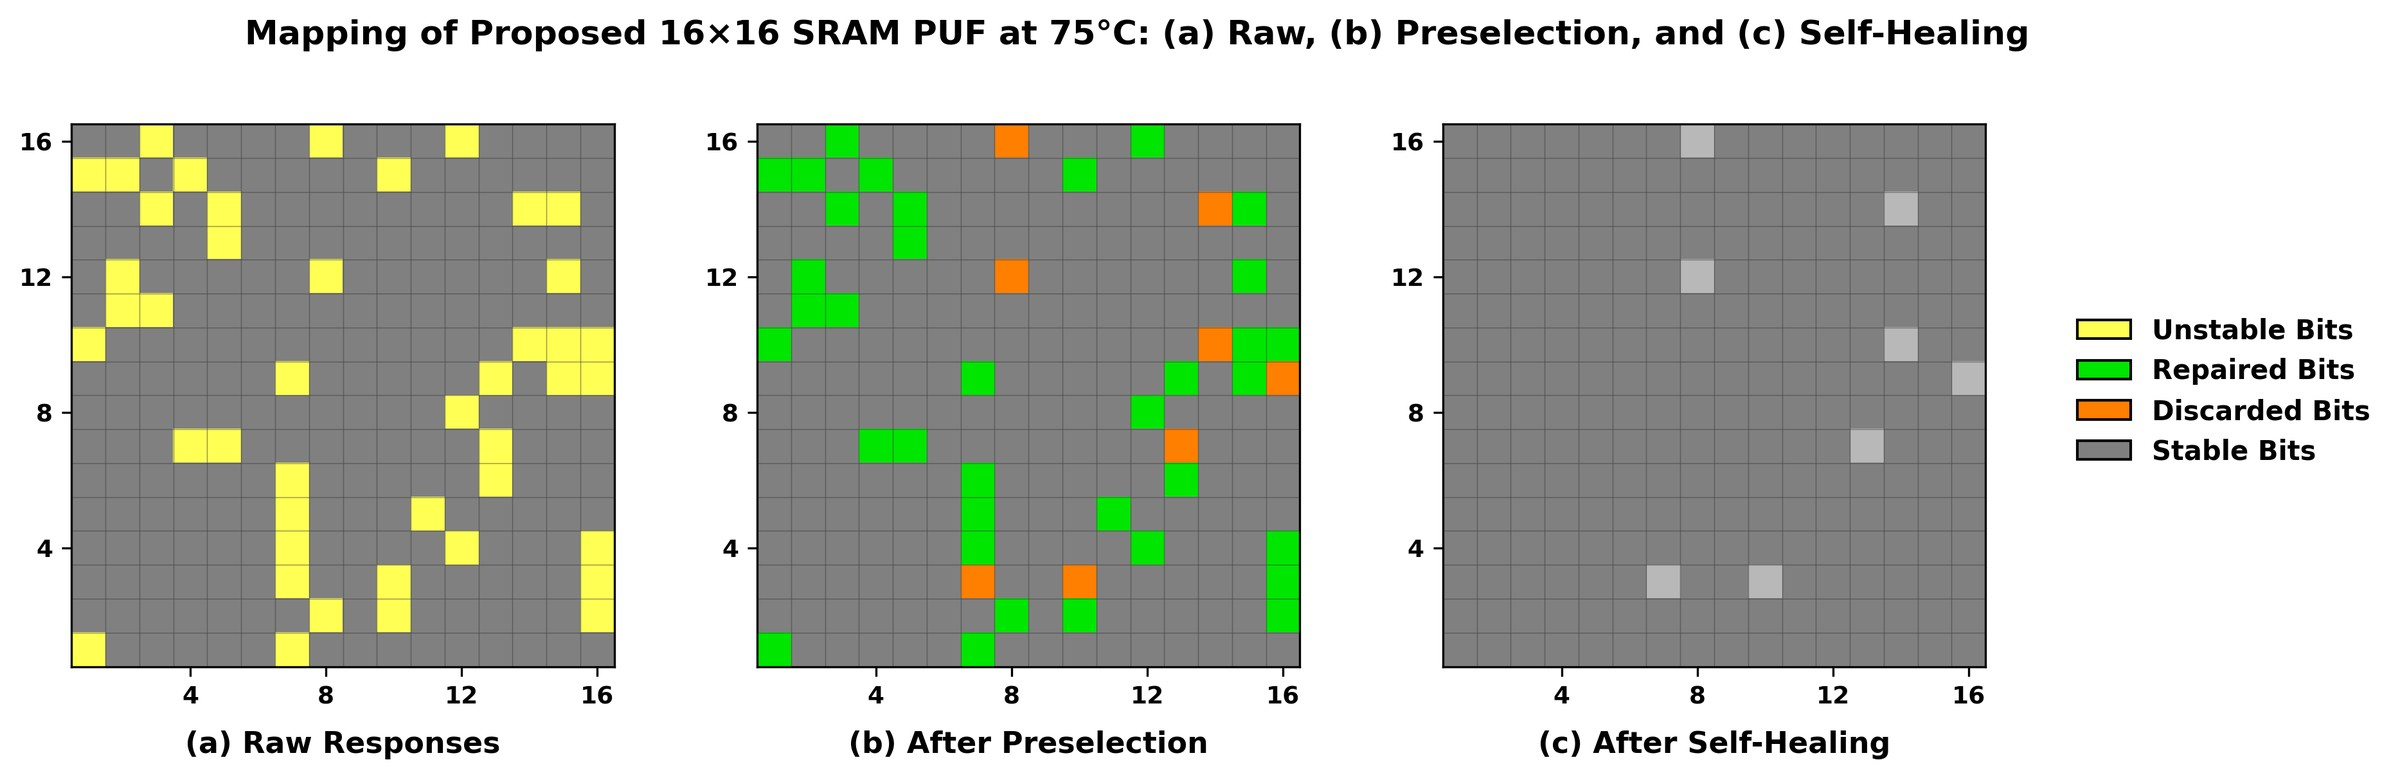
\includegraphics[width=0.49\textwidth]{nb33_map16_T75C.jpg}
\caption{16$\times$16 maps at $-100\,^\circ$C (left; 3 unstable, all repaired) and $75\,^\circ$C (right; 44 unstable, 36 repaired, 8 discarded), 0.9\,V, $\pm120$\,mV.}
\label{fig:tmaps}
\end{figure*}

\subsection{Flip Direction}
Every flip follows the tilt sign (Fig.~\ref{fig:flip}; all twenty-one runs are in \path{results/directional_flips_vs_golden_key.csv}): a positive tilt produces 1$\rightarrow$0 flips and a negative tilt 0$\rightarrow$1 flips; at 0.9\,V, $+120$\,mV flips 14 bits 1$\rightarrow$0 and $-120$\,mV flips 16 bits 0$\rightarrow$1. Supply alone also biases the cell: with no tilt all six errors at 0.8\,V are 0$\rightarrow$1 and all four at 1.0\,V are 1$\rightarrow$0.

\subsection{Temperature}
Tables~\ref{tab:tdist} and \ref{tab:tber} and Figs.~\ref{fig:yield}--\ref{fig:tmaps} cover $-100$ to 75\,$^\circ$C at 0.9\,V. The same $\pm120$-mV tilt flags 3 cells at $-100\,^\circ$C and 44 at 75\,$^\circ$C, consistent with the latch's regenerative gain falling with temperature so that mismatch margins shrink relative to the tilt. Healing efficiency is 96--100\% up to 27\,$^\circ$C and 81.8\% at 75\,$^\circ$C, where 8 cells are unstable in both modes and the valid yield is 96.88\%. The healed key's Hamming weight stays at 54.4--55.5\%.

Measured against each temperature's own nominal key, the mean raw Mode~1 tilt BER grows from 0.26\% to 6.12\% and its 128-bit BLER from 28\% to almost 100\%. After healing, without masking, the mean BER is 0.00\% at $-100$ and $-40\,^\circ$C, 0.13\% at 0 and 27\,$^\circ$C and 0.91\% at 75\,$^\circ$C, giving 128-bit BLERs of 0, 15.4 and 69.0\%. The nominal Mode~1 key at $-100\,^\circ$C differs from the 27\,$^\circ$C key in 1.56\% of bits, at $-40\,^\circ$C in 0.39\%, and not at all at 0 or 75\,$^\circ$C. Discarding the dark bits leaves no errors at any temperature, by construction.

\begin{table}[!t]
\caption{Bit Classification Against Temperature (0.9\,V, $\pm$120\,mV)}
\label{tab:tdist}
\centering
\footnotesize
\setlength{\tabcolsep}{3.4pt}
\begin{tabular}{@{}rrrrrrr@{}}
\toprule
$T$ ($^\circ$C) & Unstable & Rep. & Disc. & Heal eff. & Yield & HW \\
\midrule
$-100$ & 3 (1.17\%) & 3 & 0 & 100\% & 100\% & 55.47\% \\
$-40$ & 15 (5.86\%) & 15 & 0 & 100\% & 100\% & 55.47\% \\
0 & 27 (10.55\%) & 26 & 1 & 96.30\% & 99.61\% & 54.90\% \\
27 & 30 (11.72\%) & 29 & 1 & 96.67\% & 99.61\% & 55.29\% \\
75 & 44 (17.19\%) & 36 & 8 & 81.82\% & 96.88\% & 54.44\% \\
\bottomrule
\end{tabular}
\end{table}

\begin{table}[!t]
\caption{Mean Tilt BER and BLER Against Temperature}
\label{tab:tber}
\centering
\footnotesize
\setlength{\tabcolsep}{2.8pt}
\begin{tabular}{@{}rrrrrrr@{}}
\toprule
$T$ & Drift & Raw M1 & Raw M2 & Healed & BLER$_{128}$ & BLER$_{128}$ \\
($^\circ$C) & vs.\ 27\,$^\circ$C & (\%) & (\%) & (\%) & raw (\%) & healed (\%) \\
\midrule
$-100$ & 1.56 & 0.26 & 0.72 & 0.00 & 28.38 & 0.00 \\
$-40$ & 0.39 & 1.72 & 2.11 & 0.00 & 89.13 & 0.00 \\
0 & 0.00 & 3.84 & 3.12 & 0.13 & 99.34 & 15.36 \\
27 & 0.00 & 4.23 & 3.32 & 0.13 & 99.61 & 15.36 \\
75 & 0.00 & 6.12 & 5.79 & 0.91 & 99.97 & 69.03 \\
\bottomrule
\multicolumn{7}{@{}p{0.95\columnwidth}@{}}{\scriptsize BER against the same-temperature nominal key, mean over tilts; healed is unmasked. 256-bit BLER is in \path{results/temperature_ber_bler_summary.csv}.}
\end{tabular}
\end{table}

\begin{figure}[!t]
\centering
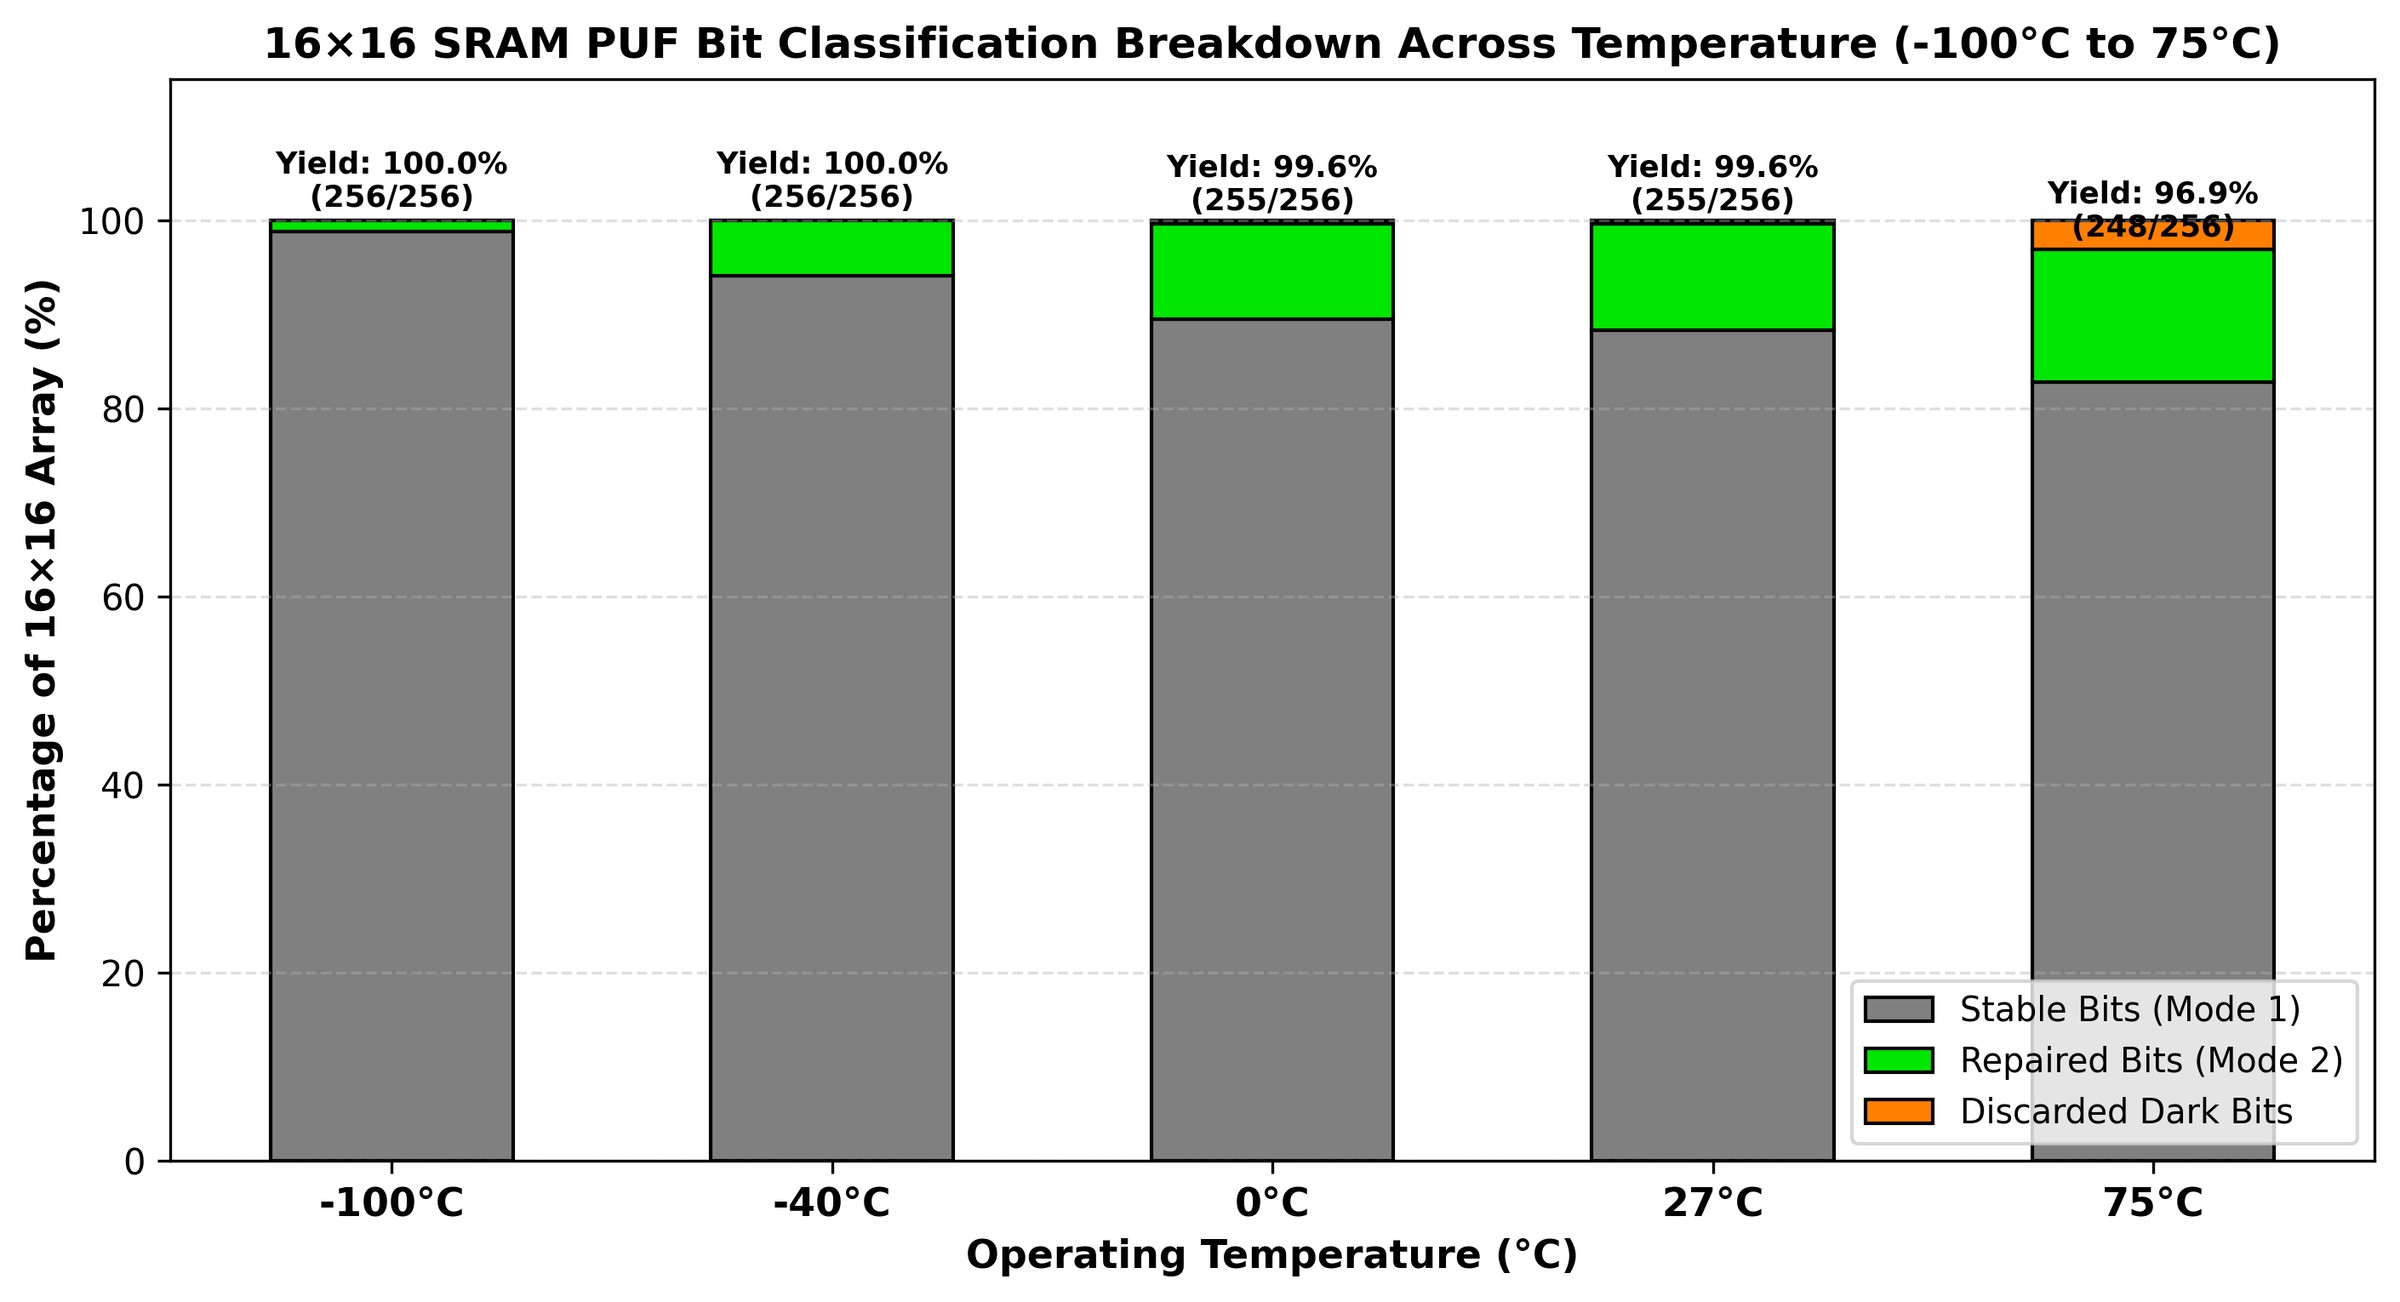
\includegraphics[width=0.95\columnwidth]{nb33_yield_breakdown_vs_temperature.jpg}
\caption{Stable, repaired and discarded cells against temperature; labels give the valid-bit yield.}
\label{fig:yield}
\end{figure}

\begin{table*}[!t]
\caption{This Work Against Chen et al. \cite{chen2024}}
\label{tab:paper}
\centering
\footnotesize
\begin{tabular}{@{}>{\raggedright\arraybackslash}p{0.21\textwidth}>{\raggedright\arraybackslash}p{0.25\textwidth}>{\raggedright\arraybackslash}p{0.29\textwidth}>{\raggedright\arraybackslash}p{0.17\textwidth}@{}}
\toprule
Quantity & Chen et al. (silicon) & This work (simulation) & Comparable? \\
\midrule
Technology, supply, array & 55\,nm, 1.2\,V, 64$\times$64, 5 chips & UMC 28\,nm, 0.9\,V, 16$\times$16 and 32$\times$64 & Setup differs \\
Cell & 15T multimode, 2763\,F$^2$ & 15T multimode, schematic level & Same topology \\
Tilt generator & 7-bit capacitive DAC & 7-bit capacitive DAC (10--640\,fF) & Same \\
Tilt for preselection & $\Vd=80$\,mV & 50, 80, 120\,mV & Yes at 80\,mV \\
Native BER at nominal, raw/healed & 0.863\% / 0.136\% & 0\% / 0\% (no transient noise; golden key is this run) & No \\
Unstable bits at nominal, raw/healed & 5.102\% / 1.635\% (1000 reads) & 8.20\% / 0\% (flagged by $\pm80$\,mV tilt) & Different definitions \\
Worst BER over supply, raw/healed & 3.11\% / 1.23\% (1.08--1.32\,V) & 2.34\% / 0\% (0.8--1.0\,V, no tilt) & Trend yes \\
Worst BER over temperature, raw/healed & 3.76\% / 0.72\% ($-40$ to 125\,$^\circ$C) & 6.12\% / 0.91\% mean tilt BER at 75\,$^\circ$C; nominal drift $\le$1.56\% & Trend yes \\
Healing-only BER reduction & 2.7$\times$ / 2.3$\times$ after 100\,krad(Si) & 3.3$\times$ (0.9\,V) and 3.6$\times$ (0.8\,V) at $\pm120$\,mV & Same order \\
Unstable bits at maximum stress, raw/healed & 14.62\% / 4.675\% (Chip~1, 100\,krad) & 11.72\% / 3.52\% (0.9\,V, $\pm120$\,mV) & Proxy only \\
Bits discarded after healing & not stated & 0.98\% (32$\times$64, $\pm120$\,mV); 3.1\% at 75\,$^\circ$C & n/a \\
Masking for zero BER & 25--32\% masked & 0\% with tilt+V mask, in sample & No \\
Final BER with heal + masks & 0.0168\% / 0.0183\% after 100\,krad & --- & Not studied \\
Dominant flip direction & 1$\rightarrow$0 (4.26 vs.\ 1.68\%, Chip~1) & follows tilt sign; symmetric overall & No (symmetric stress) \\
Two modes independent & claimed; not quantified & inter-mode HD 48.8\%; discards 20 vs.\ 23 expected & Supports claim \\
Uniformity / uniqueness & inter-die HD 0.494 (healed 0.4835) & HW 54--57\%; one array & Partly \\
Randomness & NIST SP 800-22: 10/10 passed & not tested & No \\
Power, energy & 0.20\,$\mu$W/bit static; 140\,fJ/b & not measured & No \\
\bottomrule
\end{tabular}
\end{table*}

\section{Comparison of Results}
\label{sec:compare}
\subsection{Within This Work}
\emph{Mode~1 against Mode~2.} The two modes' keys differ in 48.8\% of bit positions, and the number of cells unstable in both modes in the 32$\times$64 array (20) is close to the 23 expected for independent modes. At 27\,$^\circ$C Mode~2 is never less stable than Mode~1: at 0.9\,V, $\pm120$\,mV, 8.98\% of cells are unstable in Mode~2 against 11.72\% in Mode~1, and raw Mode~2 BER is at or below raw Mode~1 BER at every supply and tilt (Table~\ref{tab:ber}). The order reverses at low temperature, where raw Mode~2 BER is higher (0.72 against 0.26\% at $-100\,^\circ$C, 2.11 against 1.72\% at $-40\,^\circ$C). Mode~2 also has more ones (57.0 against 54.3\%).

\emph{Tilt magnitude.} At 0.8 and 0.9\,V the unstable fraction grows roughly linearly with $|\Vd|$ (4.7, 6.6, 11.3\% and 5.5, 8.2, 11.7\% for 50, 80, 120\,mV). At 1.0\,V it peaks at $\pm80$\,mV (8.98\%) and is 7.42\% at $\pm120$\,mV. Discards appear only at 0.9\,V, $\pm120$\,mV and at 1.0\,V, $\pm50$ and $\pm80$\,mV, so a larger tilt mainly costs healing effort rather than yield.

\emph{Supply against temperature.} At $\pm120$\,mV the unstable fraction barely changes between 0.8 and 0.9\,V (11.3 and 11.7\%) but varies fifteen-fold with temperature (1.2\% at $-100\,^\circ$C to 17.2\% at 75\,$^\circ$C). Temperature is therefore the dominant stress for this cell, and 75\,$^\circ$C is the only condition where healing efficiency falls below 90\%. Supply sets the direction of nominal errors (0$\rightarrow$1 at 0.8\,V, 1$\rightarrow$0 at 1.0\,V); tilt sets the direction of tilt errors.

\emph{16$\times$16 against 32$\times$64.} At 0.9\,V, $\pm120$\,mV the two arrays give 11.72 and 10.30\% unstable, 96.7 and 90.5\% healing efficiency, and 0.39 and 0.98\% discarded. The differences are within the sampling error of 256 cells (one cell is 0.39\%; the binomial standard deviation of an 11\% fraction is 2.0 points), so the larger array gives the more precise figures.

\emph{Consistency.} The 27\,$^\circ$C row of the temperature sweep reproduces the 0.9-V, $\pm120$-mV map exactly (30 unstable, 29 repaired, 1 discarded), and the healing map of the summary analysis reproduces the 0.9-V, $\pm80$-mV map (21 repaired). At 0.9\,V the unstable fraction equals twice the BER at every tilt.

\emph{Healing in and out of sample.} With healing chosen at 0.9\,V, $\pm80$\,mV, the healed BER is zero at that condition and at $\pm50$\,mV by construction. Elsewhere it is 0.20--1.76\%, against 2.73--5.86\% raw, a reduction of 3--4$\times$.

\subsection{Against Chen et al.}
Table~\ref{tab:paper} sets the main results beside those of \cite{chen2024}. The comparison is of trends, not absolute values: the paper measures 55-nm silicon at 1.2\,V with temporal noise and radiation, whereas this work simulates the same topology in 28\,nm at 0.9\,V without transient noise and uses supply tilt as the stress.

The mechanism agrees. Mode switching recovers most cells flagged by the tilt (90--100\% here; in \cite{chen2024} healing lowers the nominal unstable fraction from 5.10 to 1.64\%), and healing cuts BER under stress by a factor of 2--4 in both studies. BER rises away from the enrollment condition in both, with temperature the larger effect here. Both also show that healing alone does not reach a usable key error rate: the healed 128-bit BLER is 15\% at 27\,$^\circ$C and 69\% at 75\,$^\circ$C here, and \cite{chen2024} needs pre-irradiation masks and ECC for its final 0.018\%.

The differences follow from the setup. Without transient noise the simulated nominal BER is zero, so the paper's 0.863\% native BER and its growth with the number of reads cannot appear. A symmetric tilt cannot reproduce the radiation-induced dominance of 1$\rightarrow$0 flips. Uniqueness across chips, randomness, power and area need several dies, longer keys or layout.

\section{Limitations and Future Work}
Each Monte Carlo condition is a single deterministic transient, so temporal noise, and with it the nominal BER, is not represented; transient-noise runs with temporal majority voting would add it. Supply tilt serves as an enrollment stress, not as a model of ionizing dose. One array instance is simulated, so inter-chip Hamming distance, autocorrelation and NIST randomness tests are not yet available, and in the 16$\times$16 array one error is 0.39\%. Masks should be evaluated on held-out conditions with their masking ratio reported. Planned work \cite{phase0,phase2}: uniqueness and reliability across several Monte Carlo chip instances, process-corner and wider voltage/temperature robustness, a sweep of $\Vd$ against discarded bits and residual BER, emulation of total-ionizing-dose effects as unequal threshold-voltage shifts, and a bias-aware tilt that targets the 1$\rightarrow$0 direction.

\section{Conclusion}
A 16$\times$16 dual-mode self-healing SRAM PUF was designed in UMC 28-nm CMOS with its full periphery: a 7-bit capacitive tilt DAC, row decoding and mode/wordline drivers, precharge and write drivers, sense-amplifier key readout and a stability-decision circuit. The blocks, a 2$\times$2 test array and the full array were verified in simulation. Monte Carlo analysis shows that the two modes behave as independent responses (48.8\% inter-mode distance; discards close to the independence estimate) and that mode switching recovers 90--100\% of the cells flagged by voltage-tilt preselection at room temperature, keeping valid yield at or above 99\%, and 96.9\% at 75\,$^\circ$C. Outside its enrollment condition healing cuts BER by 3--4$\times$; under supply tilt the mean healed BER is 0\% at $-100$ and $-40\,^\circ$C, 0.13\% at 0 and 27\,$^\circ$C and 0.91\% at 75\,$^\circ$C, against 0.26--6.12\% raw. These trends match the silicon results of Chen \emph{et al.}, while the absolute numbers differ because this study has no temporal noise, no radiation and a single array.

\appendices
\section{All Notebook Figures}
Figures~\ref{fig:app27}--\ref{fig:appextra} reproduce every notebook plot not shown above, so that all 24 appear in the report. Table~\ref{tab:inventory} lists each with its notebook cell.

\begin{table}[!h]
\caption{Notebook Figure Inventory}
\label{tab:inventory}
\centering
\scriptsize
\setlength{\tabcolsep}{2.5pt}
\begin{tabular}{@{}lll@{}}
\toprule
Cell & Content & Figure \\
\midrule
18, 19, 20 & 16$\times$16 maps, 0.9\,V, $\pm80$, $\pm50$, $\pm120$\,mV & \ref{fig:maps}, \ref{fig:app27} \\
21, 22, 23 & 16$\times$16 maps, 1.0\,V, $\pm80$, $\pm120$, $\pm50$\,mV & \ref{fig:maps}, \ref{fig:app27} \\
25, 27, 29 & 16$\times$16 maps, 0.8\,V, $\pm50$, $\pm80$, $\pm120$\,mV & \ref{fig:maps}, \ref{fig:app27} \\
30 & 32$\times$64 map, 0.9\,V, $\pm120$\,mV & \ref{fig:maps} \\
31 & Healing map, 0.9\,V, $\pm80$\,mV & \ref{fig:appextra} \\
31 & BER and unstable bits vs.\ tilt & \ref{fig:bertilt} \\
31 & BER vs.\ supply & \ref{fig:bervdd} \\
31 & Flip direction, symmetric tilt & \ref{fig:appextra} \\
31 & Healing and masking vs.\ tilt & \ref{fig:bertilt} \\
32 & Directional flips, tilt and supply sweeps & \ref{fig:flip} \\
33 & Maps at $-100$, $-40$, 0, 27, 75\,$^\circ$C & \ref{fig:tmaps}, \ref{fig:apptemp} \\
33 & Yield breakdown vs.\ temperature & \ref{fig:yield} \\
34 & BER and BLER vs.\ temperature & \ref{fig:bertemp} \\
34 & Per-tilt BER vs.\ temperature & \ref{fig:bertemp} \\
\bottomrule
\end{tabular}
\end{table}

\begin{figure*}[!p]
\centering
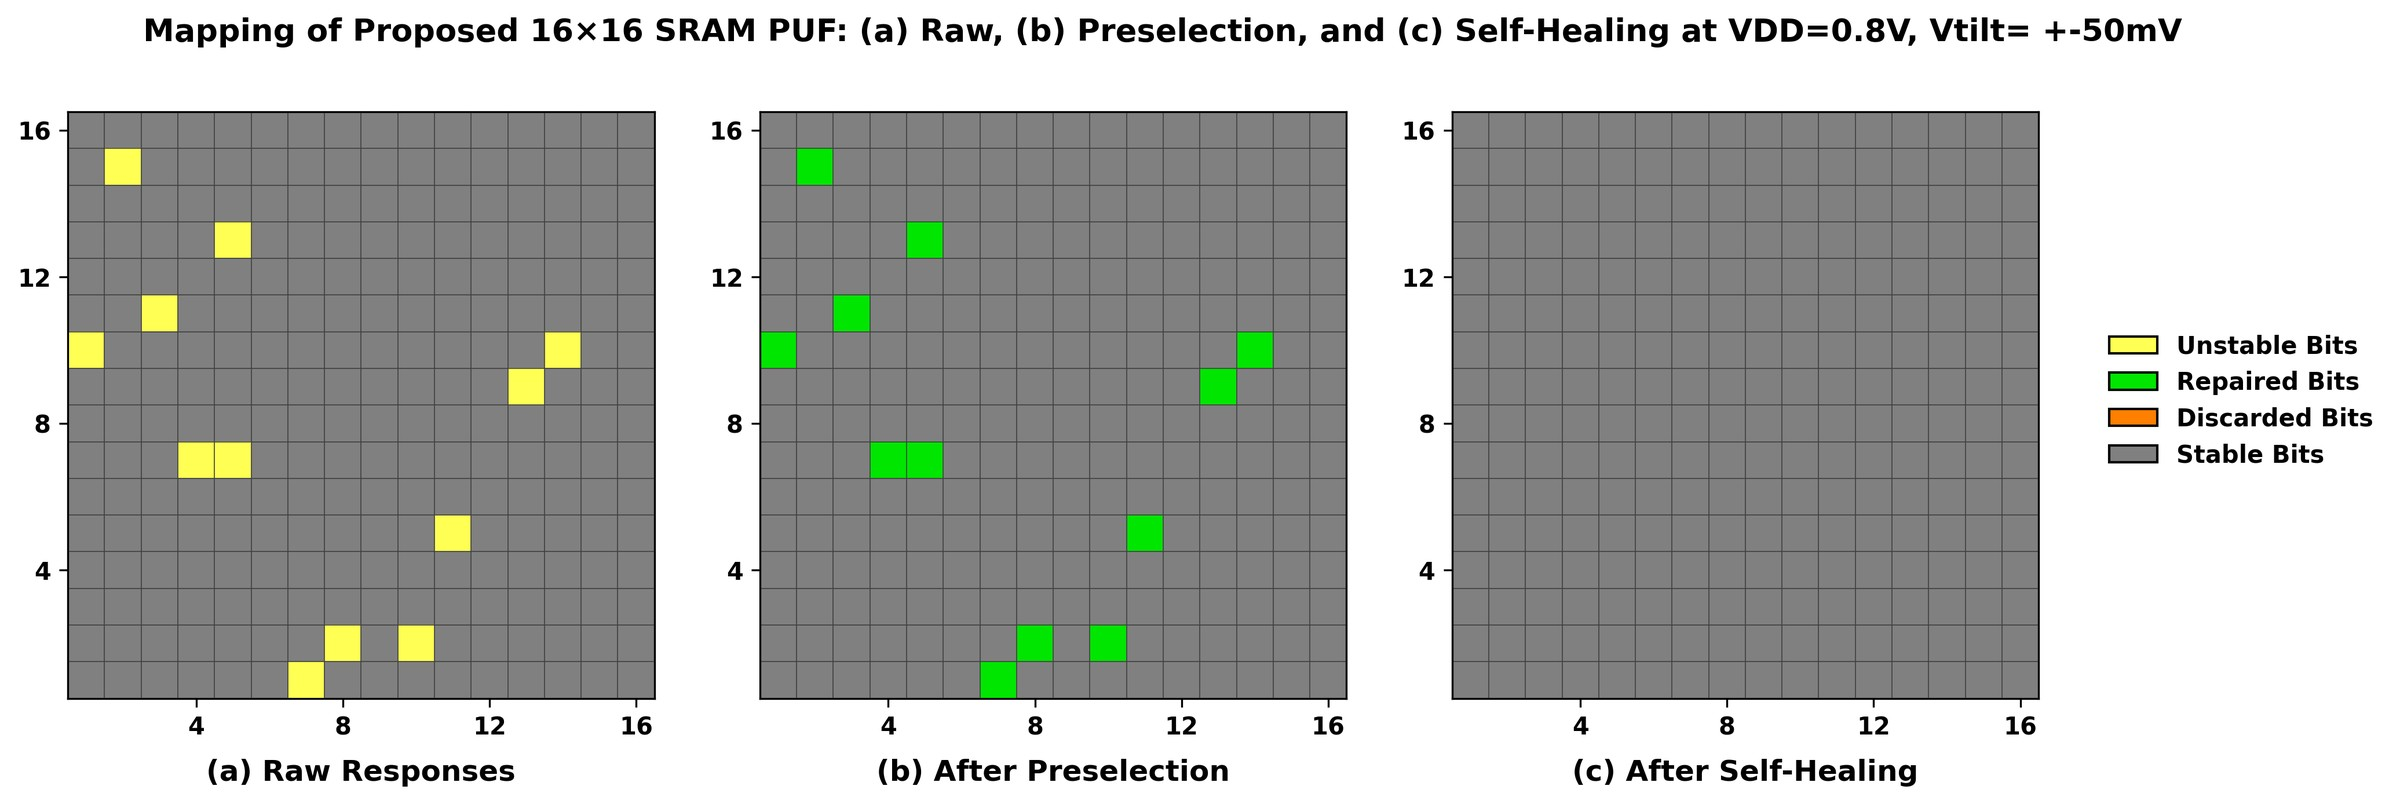
\includegraphics[width=0.49\textwidth]{nb25_map16_27C_VDD0.8_tilt50.jpg}\hfill
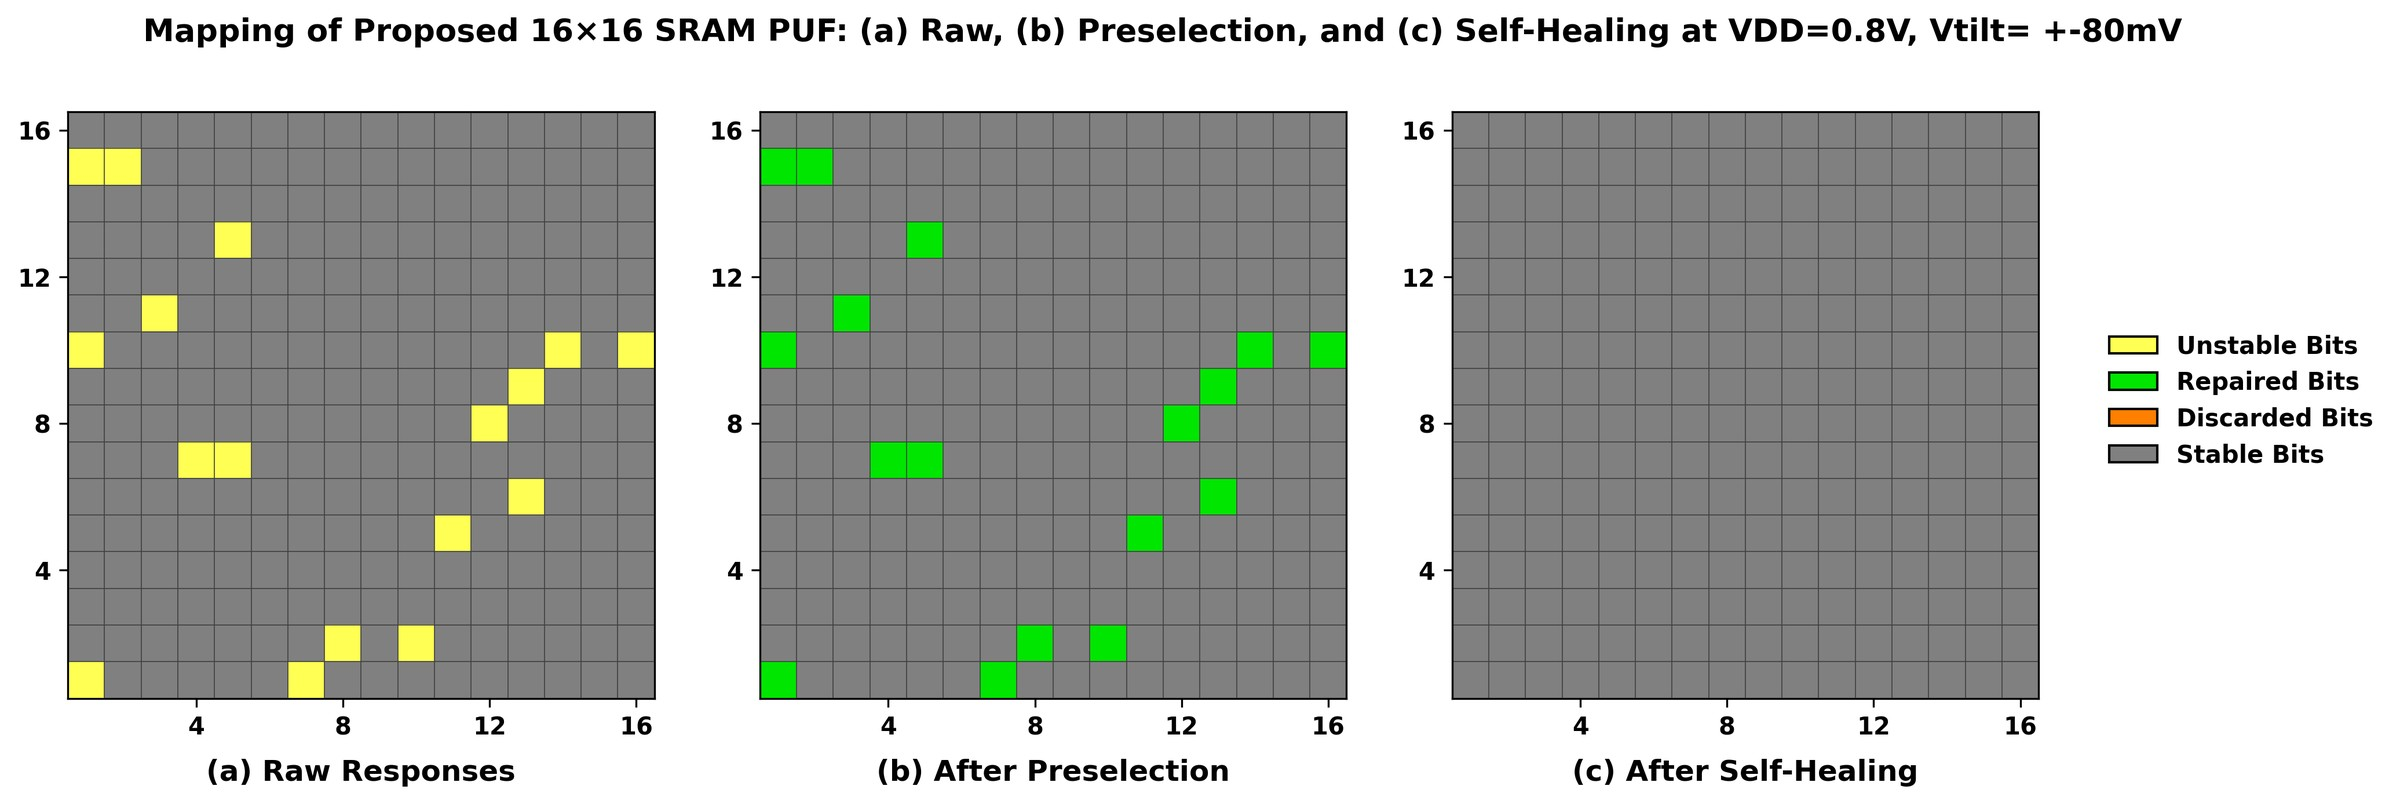
\includegraphics[width=0.49\textwidth]{nb27_map16_27C_VDD0.8_tilt80.jpg}\\[3pt]
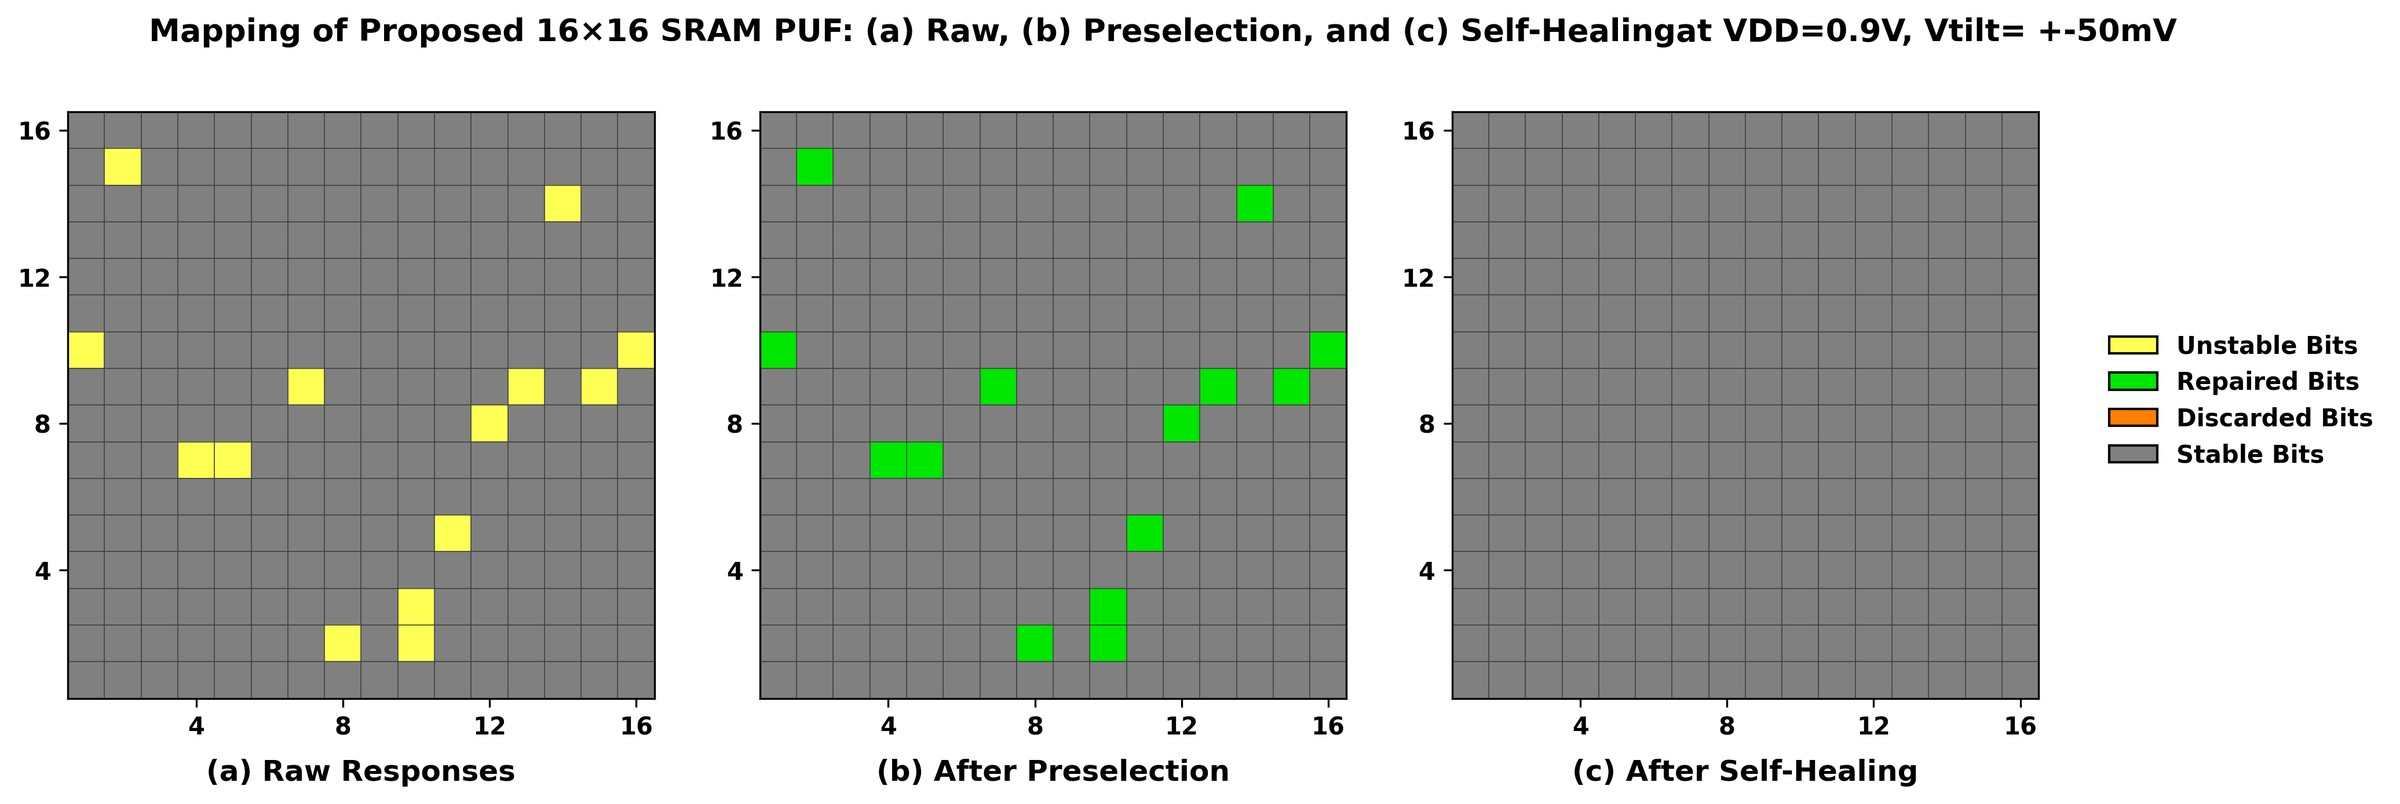
\includegraphics[width=0.49\textwidth]{nb19_map16_27C_VDD0.9_tilt50.jpg}\hfill
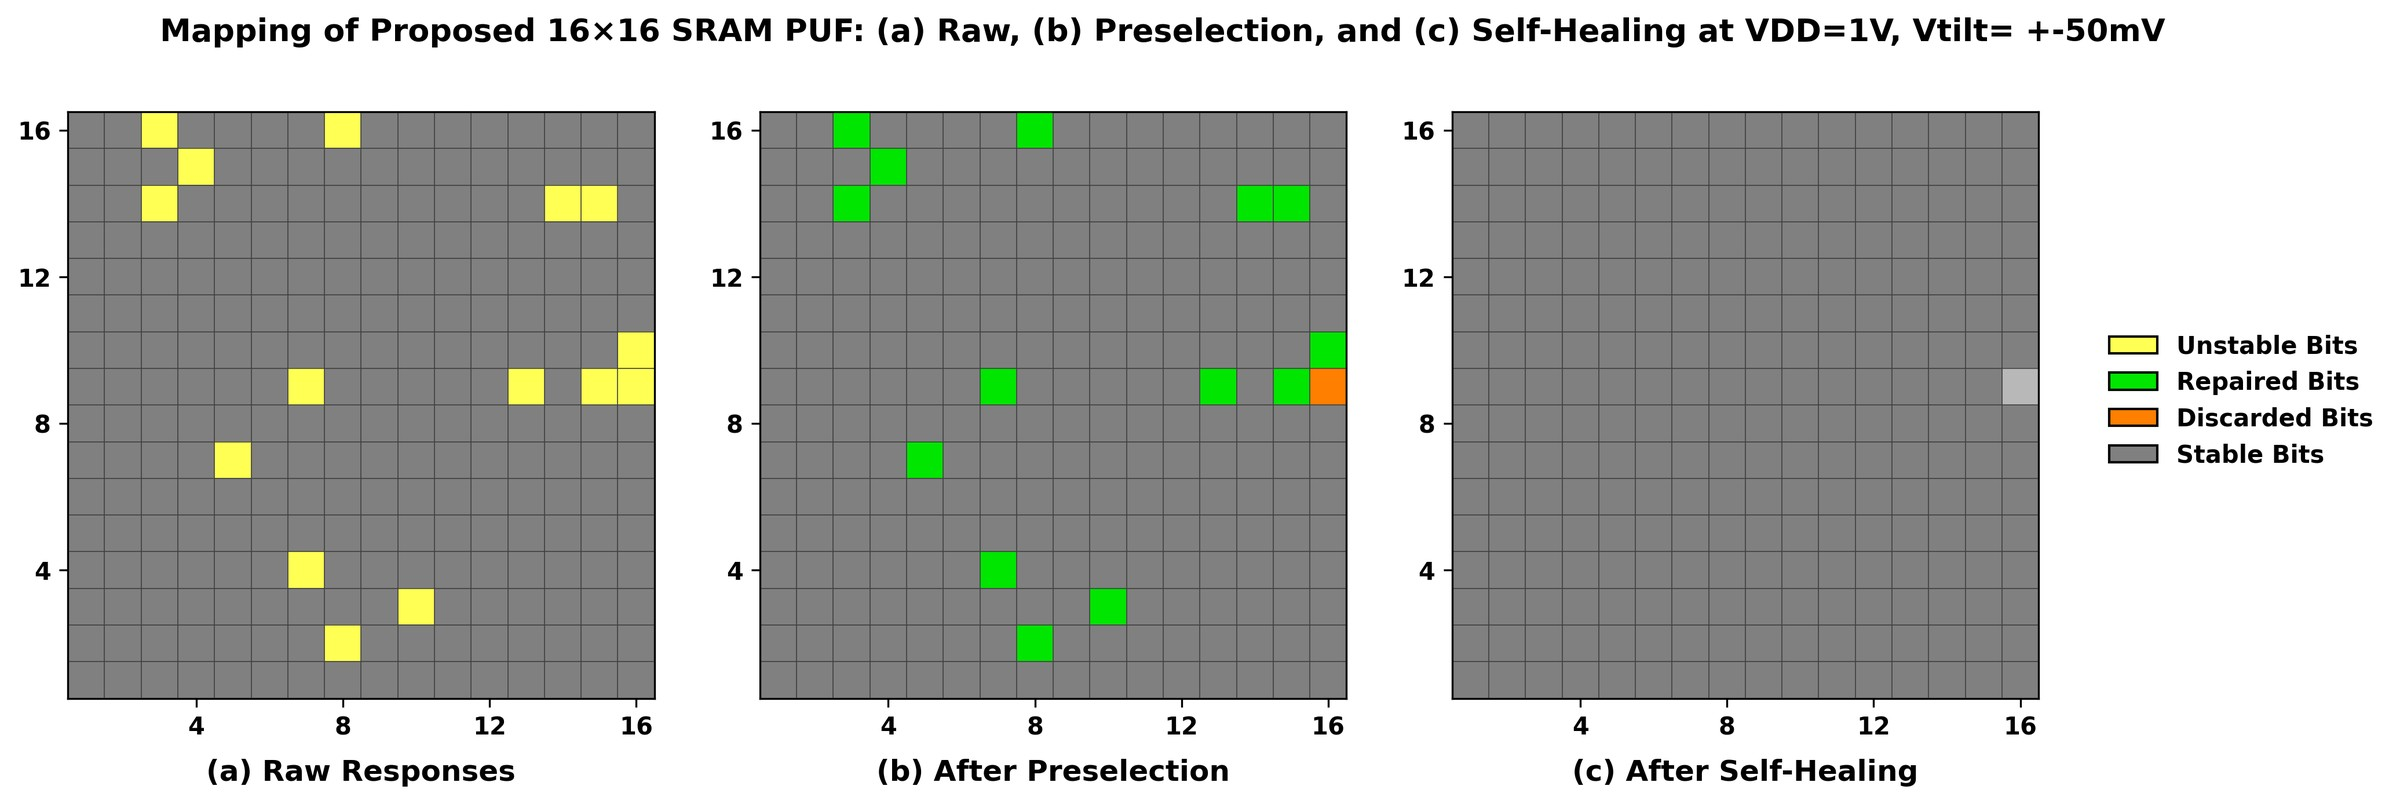
\includegraphics[width=0.49\textwidth]{nb23_map16_27C_VDD1.0_tilt50.jpg}\\[3pt]
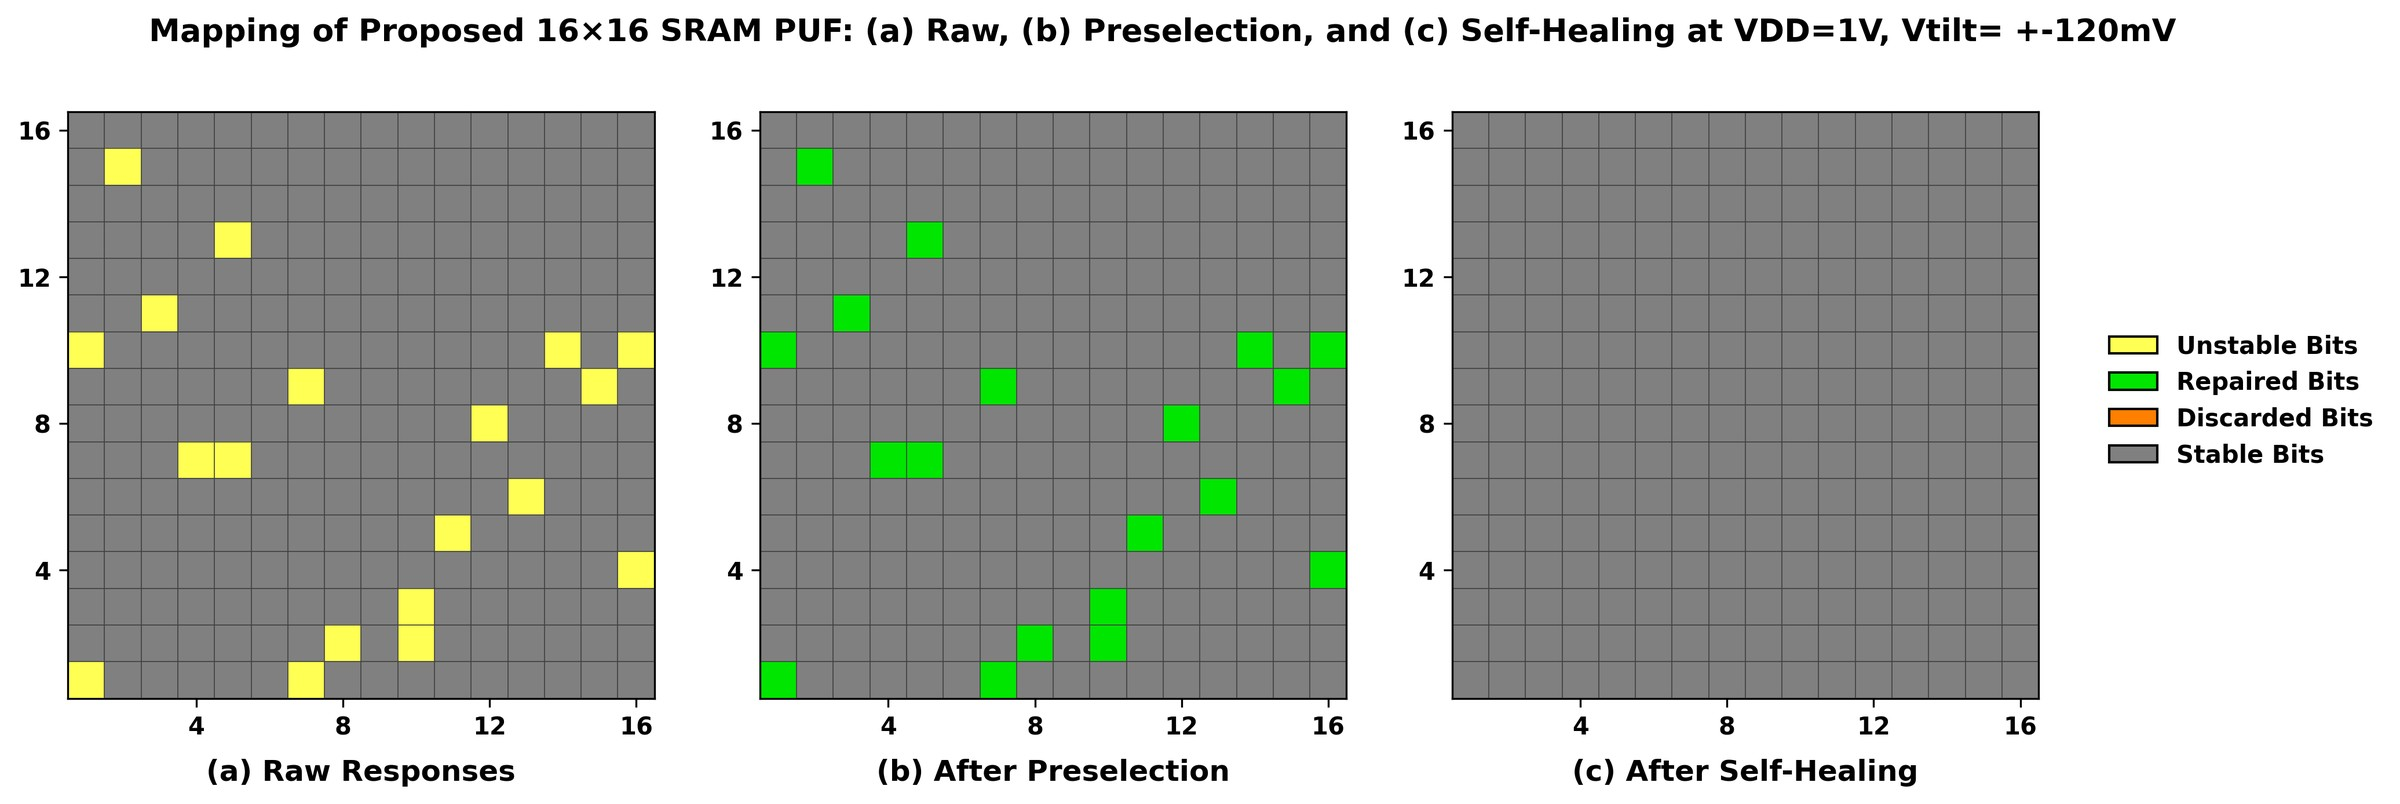
\includegraphics[width=0.49\textwidth]{nb22_map16_27C_VDD1.0_tilt120.jpg}
\caption{Remaining 27\,$^\circ$C maps of the 16$\times$16 array. Top: 0.8\,V at $\pm50$\,mV (12 unstable, all repaired) and $\pm80$\,mV (17, all repaired). Middle: 0.9\,V at $\pm50$\,mV (14, all repaired) and 1.0\,V at $\pm50$\,mV (15 unstable, 14 repaired, 1 discarded). Bottom: 1.0\,V at $\pm120$\,mV (19 unstable, all repaired).}
\label{fig:app27}
\end{figure*}

\begin{figure*}[!t]
\centering
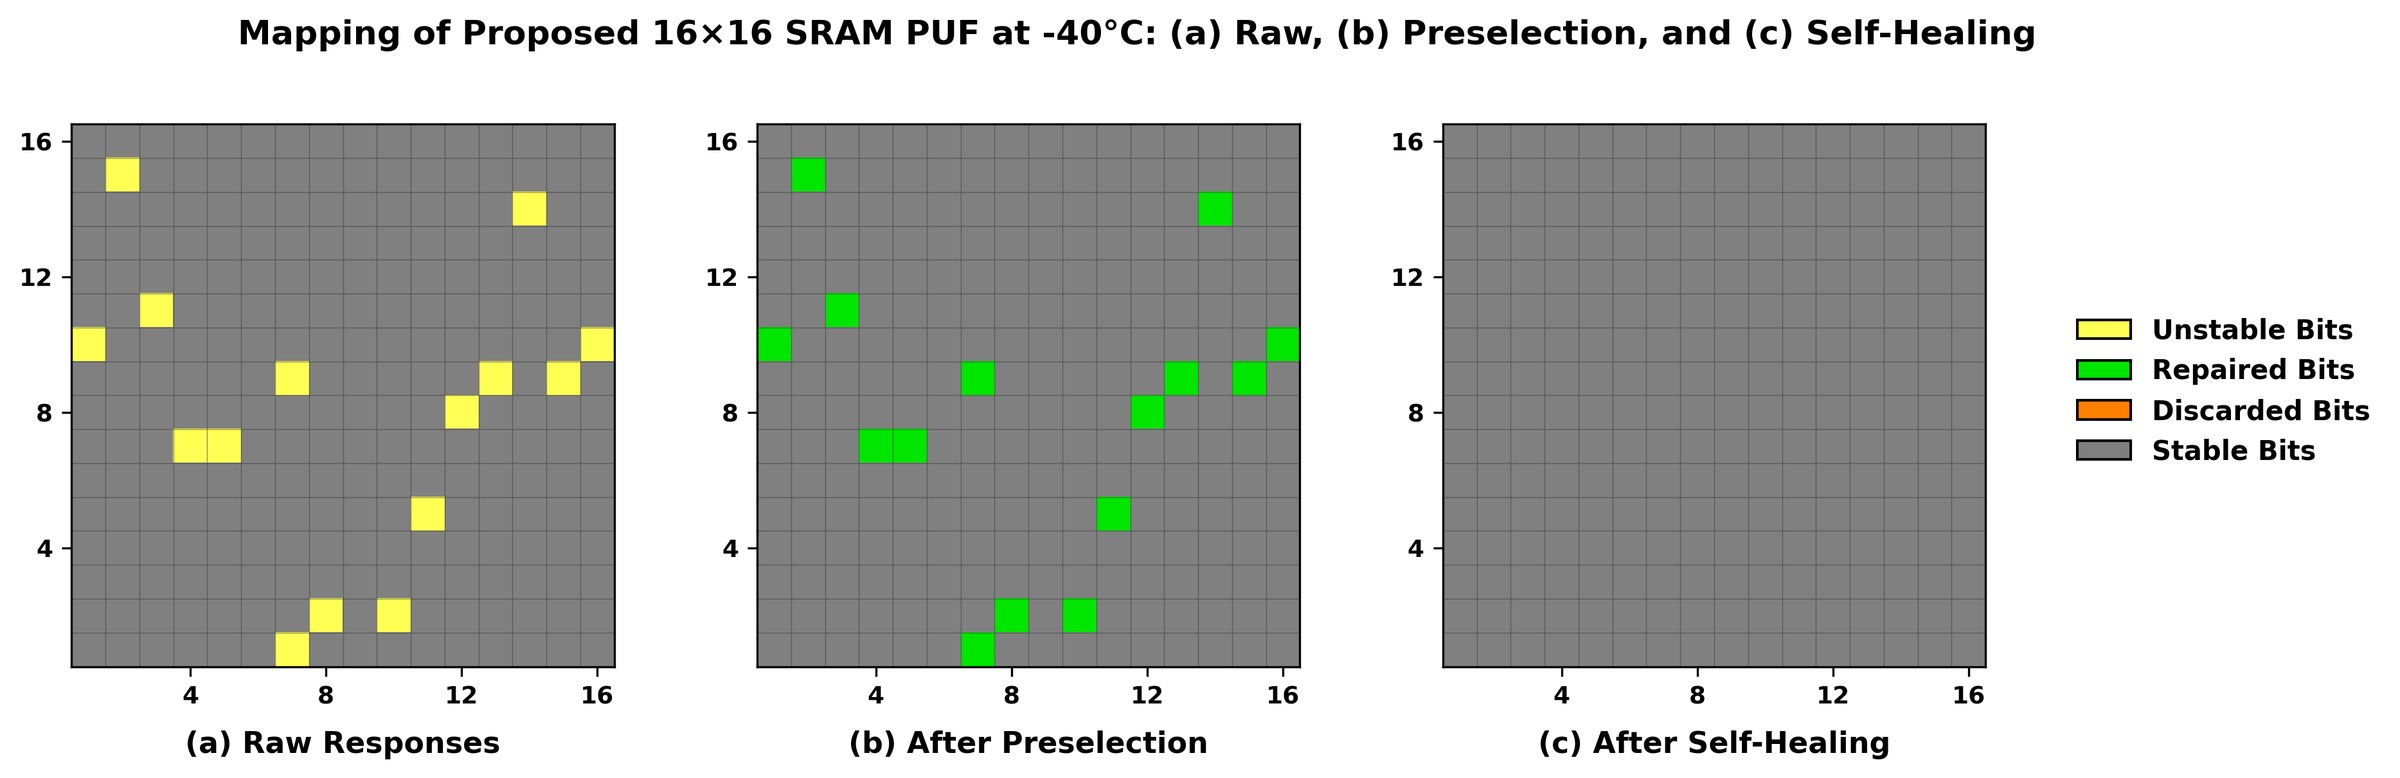
\includegraphics[width=0.49\textwidth]{nb33_map16_T-40C.jpg}\hfill
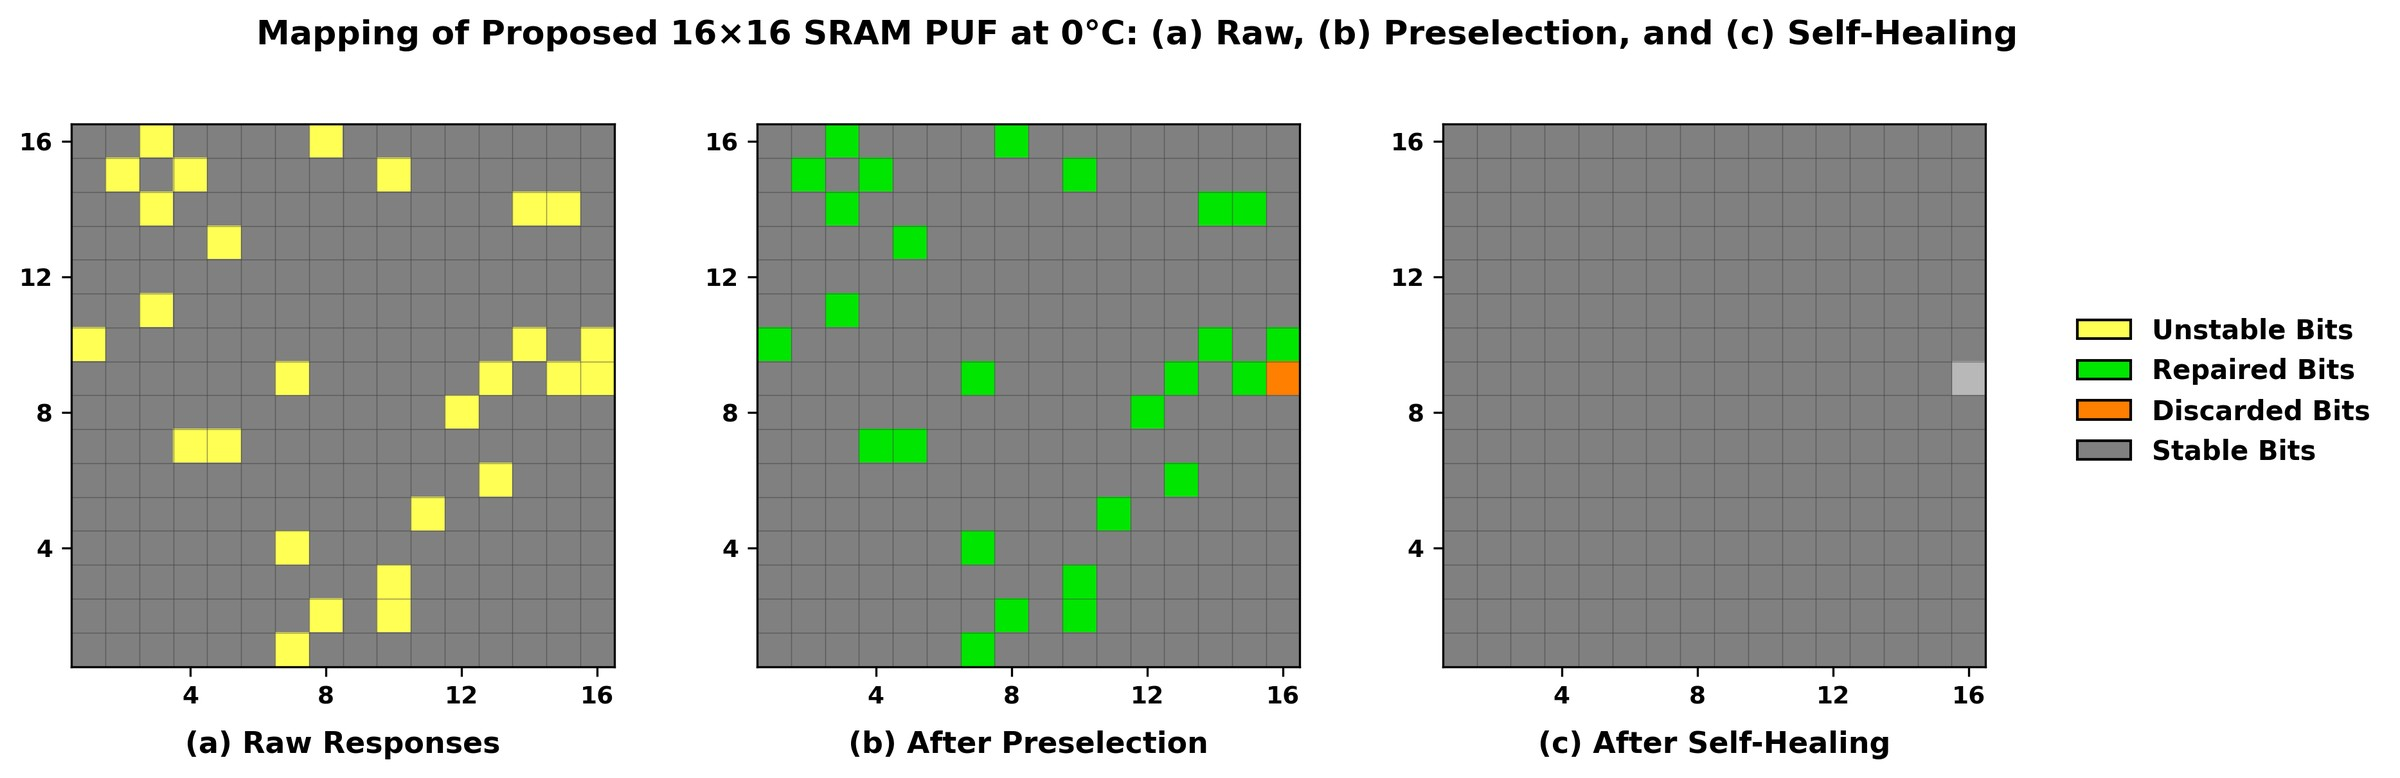
\includegraphics[width=0.49\textwidth]{nb33_map16_T0C.jpg}\\[3pt]
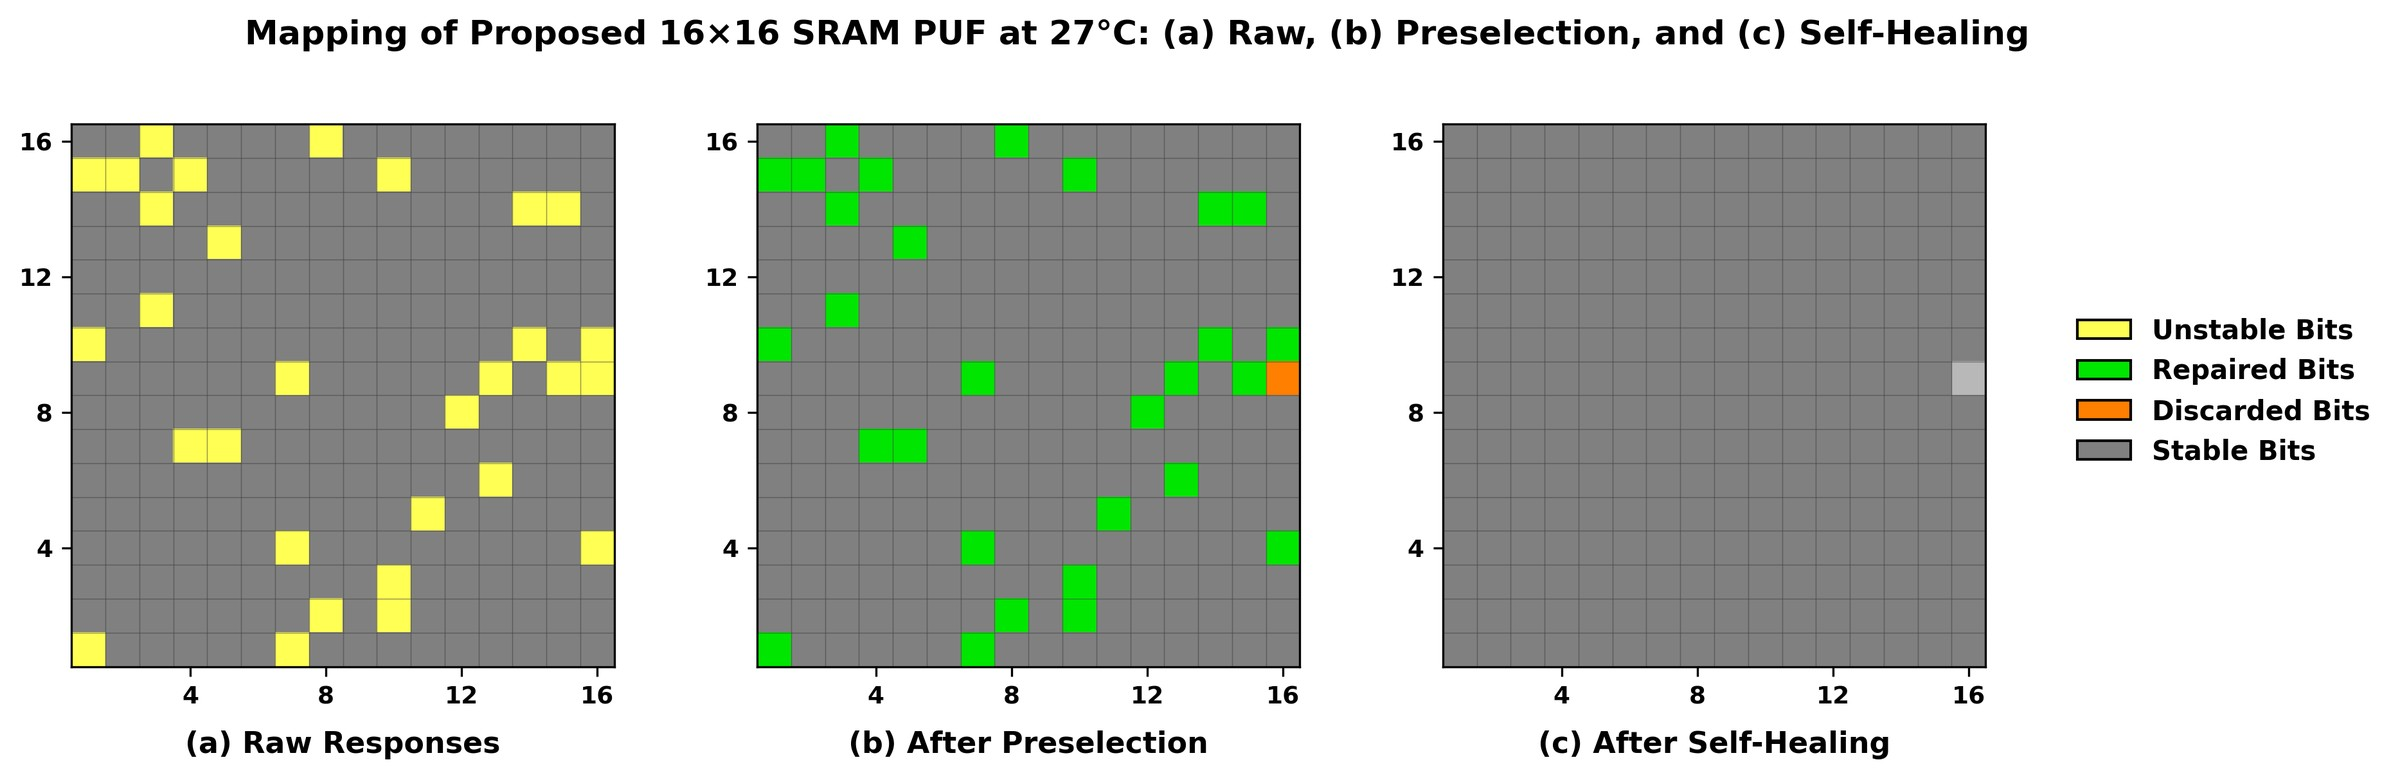
\includegraphics[width=0.49\textwidth]{nb33_map16_T27C.jpg}
\caption{Temperature maps at 0.9\,V, $\pm120$\,mV: $-40\,^\circ$C (15 unstable, all repaired), 0\,$^\circ$C (27 unstable, 26 repaired, 1 discarded) and 27\,$^\circ$C (30, 29, 1; identical to Fig.~\ref{fig:maps}, top right).}
\label{fig:apptemp}
\end{figure*}

\begin{figure*}[!t]
\centering
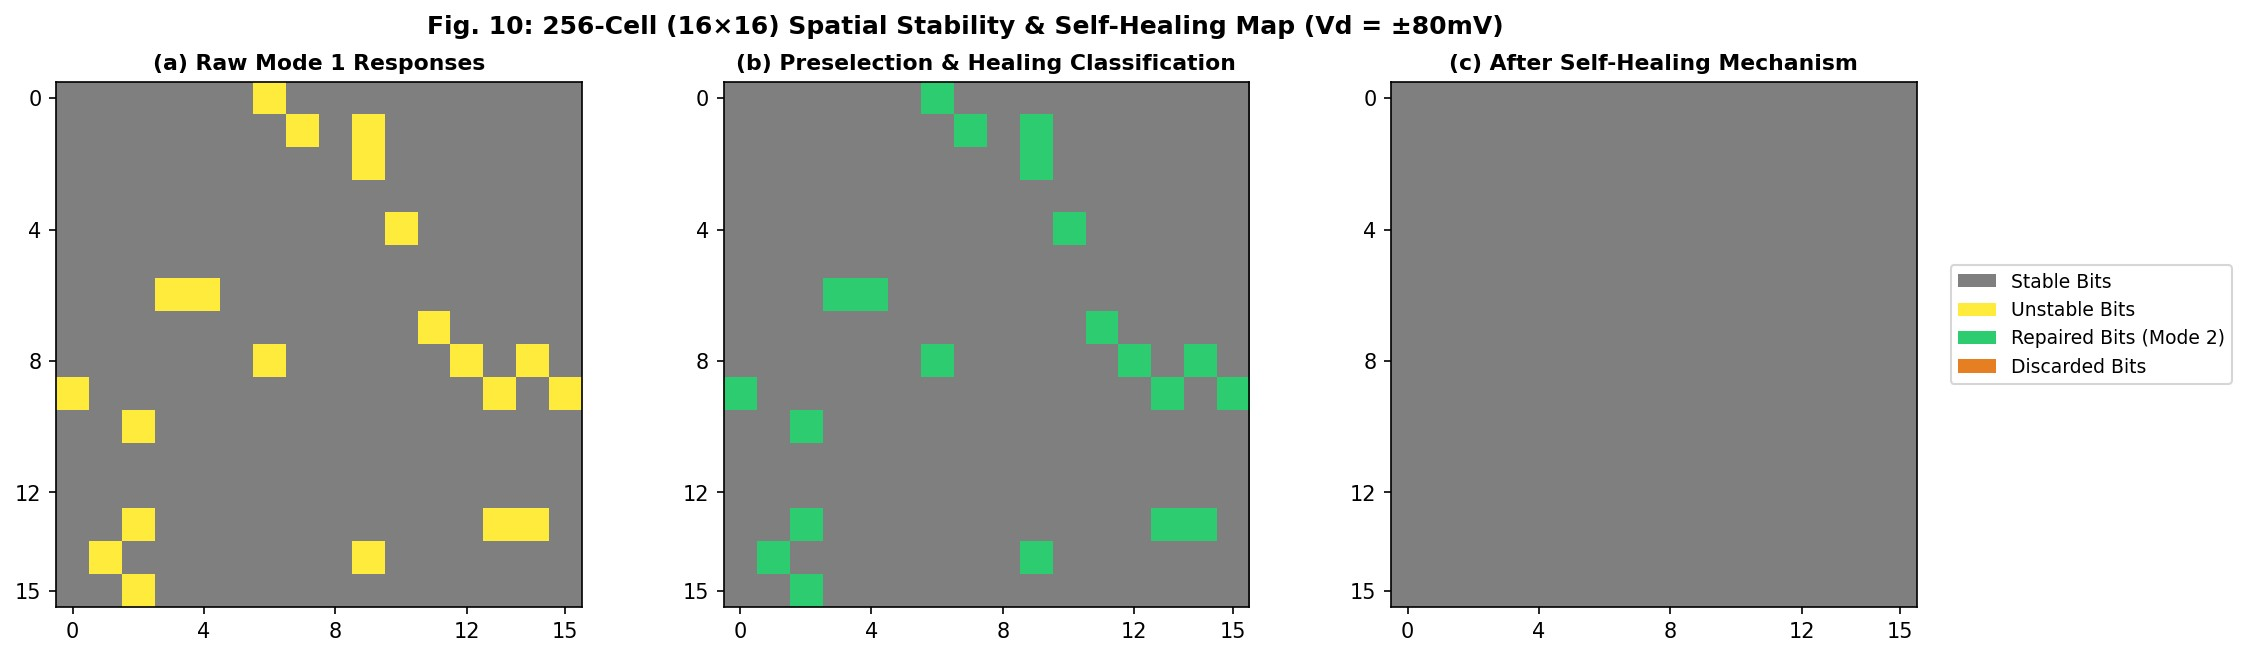
\includegraphics[width=0.48\textwidth]{nb31_healing_map_VDD0.9_tilt80.jpg}\hfill
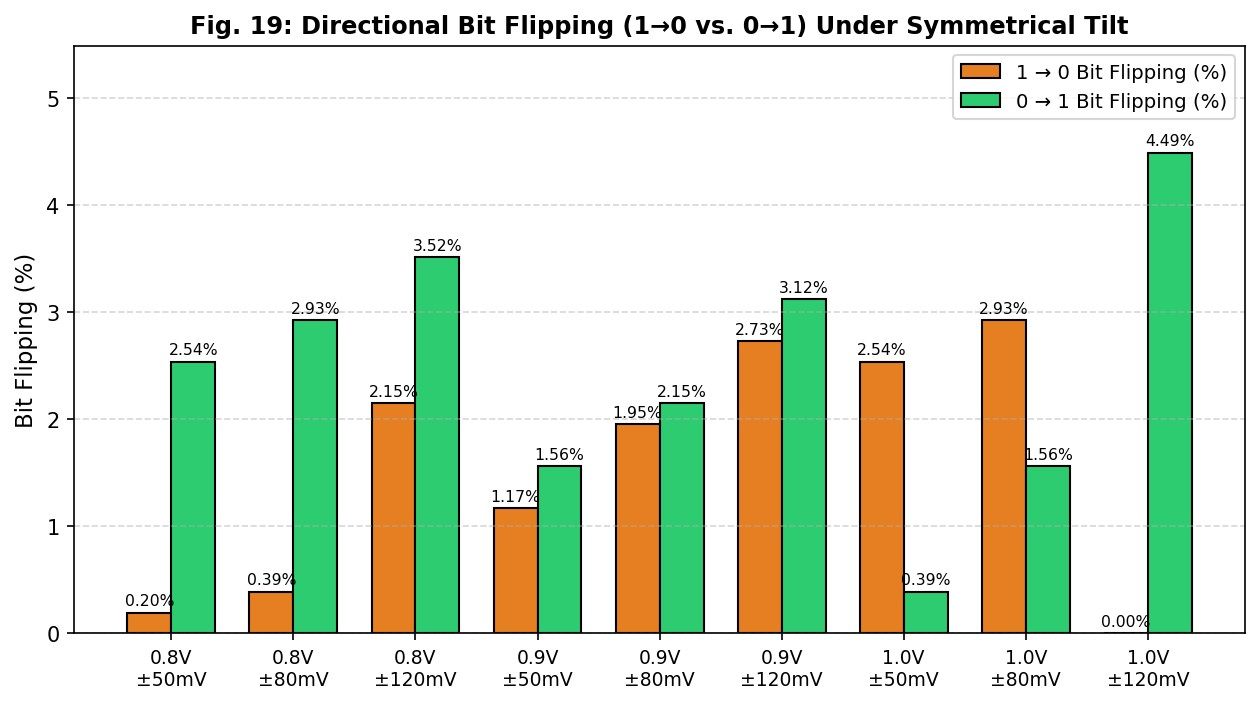
\includegraphics[width=0.44\textwidth]{nb31_flip_direction_symmetric_tilt.jpg}
\caption{Left: healing map from the summary analysis at 0.9\,V, $\pm80$\,mV (21 cells repaired by Mode~2, none discarded). Right: 1$\rightarrow$0 and 0$\rightarrow$1 flips relative to the golden key, averaged over $+$tilt and $-$tilt, for each supply and tilt magnitude.}
\label{fig:appextra}
\end{figure*}

\begin{thebibliography}{9}
\bibitem{chen2024}
Z.~Chen, W.~Yang, J.~Chen, Z.~Wang, and D.~Ding, ``Improving radiation reliability of SRAM-based physical unclonable function with self-healing and pre-irradiation masking techniques,'' \emph{IEEE Trans. Very Large Scale Integr. (VLSI) Syst.}, vol.~32, no.~2, pp.~372--381, Feb. 2024, doi: 10.1109/TVLSI.2023.3332010.
\bibitem{phase0}
H.~Goel and V.~Goel, ``Improving radiation reliability of SRAM-based physical unclonable function with self-healing and pre-irradiation masking techniques,'' EE 617 paper presentation (Phase~0), IIT Gandhinagar, Oct. 2026.
\bibitem{phase2}
H.~Goel and V.~Goel, ``16$\times$16 multimode SRAM PUF in UMC 28\,nm: architecture, schematics and simulations,'' EE 617 project presentation (Phase~2), IIT Gandhinagar, Oct. 2026.
\bibitem{he2023}
Y.~He, D.~Li, Z.~Yu, and K.~Yang, ``ASCH-PUF: A `zero' bit error rate CMOS physically unclonable function with dual-mode low-cost stabilization,'' \emph{IEEE J. Solid-State Circuits}, vol.~58, no.~7, pp.~2087--2097, Jul. 2023.
\bibitem{liu2020}
K.~Liu, Y.~Min, X.~Yang, H.~Sun, and H.~Shinohara, ``A 373~F$^2$ 0.21\%-native-BER EE SRAM physically unclonable function with 2-D power-gated bit cells and $V_{SS}$ bias-based dark-bit detection,'' \emph{IEEE J. Solid-State Circuits}, vol.~55, no.~6, pp.~1719--1732, Jun. 2020.
\bibitem{shifman2018}
Y.~Shifman, A.~Miller, O.~Keren, Y.~Weizmann, and J.~Shor, ``A method to improve reliability in a 65-nm SRAM PUF array,'' \emph{IEEE Solid-State Circuits Lett.}, vol.~1, no.~6, pp.~138--141, Jun. 2018.
\end{thebibliography}

\end{document}
